\documentclass[twoside]{book}

% Packages required by doxygen
\usepackage{fixltx2e}
\usepackage{calc}
\usepackage{doxygen}
\usepackage[export]{adjustbox} % also loads graphicx
\usepackage{graphicx}
\usepackage[utf8]{inputenc}
\usepackage{makeidx}
\usepackage{multicol}
\usepackage{multirow}
\PassOptionsToPackage{warn}{textcomp}
\usepackage{textcomp}
\usepackage[nointegrals]{wasysym}
\usepackage[table]{xcolor}

% Font selection
\usepackage[T1]{fontenc}
\usepackage[scaled=.90]{helvet}
\usepackage{courier}
\usepackage{amssymb}
\usepackage{sectsty}
\renewcommand{\familydefault}{\sfdefault}
\allsectionsfont{%
  \fontseries{bc}\selectfont%
  \color{darkgray}%
}
\renewcommand{\DoxyLabelFont}{%
  \fontseries{bc}\selectfont%
  \color{darkgray}%
}
\newcommand{\+}{\discretionary{\mbox{\scriptsize$\hookleftarrow$}}{}{}}

% Page & text layout
\usepackage{geometry}
\geometry{%
  a4paper,%
  top=2.5cm,%
  bottom=2.5cm,%
  left=2.5cm,%
  right=2.5cm%
}
\tolerance=750
\hfuzz=15pt
\hbadness=750
\setlength{\emergencystretch}{15pt}
\setlength{\parindent}{0cm}
\setlength{\parskip}{3ex plus 2ex minus 2ex}
\makeatletter
\renewcommand{\paragraph}{%
  \@startsection{paragraph}{4}{0ex}{-1.0ex}{1.0ex}{%
    \normalfont\normalsize\bfseries\SS@parafont%
  }%
}
\renewcommand{\subparagraph}{%
  \@startsection{subparagraph}{5}{0ex}{-1.0ex}{1.0ex}{%
    \normalfont\normalsize\bfseries\SS@subparafont%
  }%
}
\makeatother

% Headers & footers
\usepackage{fancyhdr}
\pagestyle{fancyplain}
\fancyhead[LE]{\fancyplain{}{\bfseries\thepage}}
\fancyhead[CE]{\fancyplain{}{}}
\fancyhead[RE]{\fancyplain{}{\bfseries\leftmark}}
\fancyhead[LO]{\fancyplain{}{\bfseries\rightmark}}
\fancyhead[CO]{\fancyplain{}{}}
\fancyhead[RO]{\fancyplain{}{\bfseries\thepage}}
\fancyfoot[LE]{\fancyplain{}{}}
\fancyfoot[CE]{\fancyplain{}{}}
\fancyfoot[RE]{\fancyplain{}{\bfseries\scriptsize Generated by Doxygen }}
\fancyfoot[LO]{\fancyplain{}{\bfseries\scriptsize Generated by Doxygen }}
\fancyfoot[CO]{\fancyplain{}{}}
\fancyfoot[RO]{\fancyplain{}{}}
\renewcommand{\footrulewidth}{0.4pt}
\renewcommand{\chaptermark}[1]{%
  \markboth{#1}{}%
}
\renewcommand{\sectionmark}[1]{%
  \markright{\thesection\ #1}%
}

% Indices & bibliography
\usepackage{natbib}
\usepackage[titles]{tocloft}
\setcounter{tocdepth}{3}
\setcounter{secnumdepth}{5}
\makeindex

% Hyperlinks (required, but should be loaded last)
\usepackage{ifpdf}
\ifpdf
  \usepackage[pdftex,pagebackref=true]{hyperref}
\else
  \usepackage[ps2pdf,pagebackref=true]{hyperref}
\fi
\hypersetup{%
  colorlinks=true,%
  linkcolor=blue,%
  citecolor=blue,%
  unicode%
}

% Custom commands
\newcommand{\clearemptydoublepage}{%
  \newpage{\pagestyle{empty}\cleardoublepage}%
}

\usepackage{caption}
\captionsetup{labelsep=space,justification=centering,font={bf},singlelinecheck=off,skip=4pt,position=top}

%===== C O N T E N T S =====

\begin{document}

% Titlepage & ToC
\hypersetup{pageanchor=false,
             bookmarksnumbered=true,
             pdfencoding=unicode
            }
\pagenumbering{alph}
\begin{titlepage}
\vspace*{7cm}
\begin{center}%
{\Large Amos\textquotesingle{} Common Libraries \\[1ex]\large 1.\+0 }\\
\vspace*{1cm}
{\large Generated by Doxygen 1.8.13}\\
\end{center}
\end{titlepage}
\clearemptydoublepage
\pagenumbering{roman}
\tableofcontents
\clearemptydoublepage
\pagenumbering{arabic}
\hypersetup{pageanchor=true}

%--- Begin generated contents ---
\chapter{Amos Single File Libraries}
\label{index}\hypertarget{index}{}\label{index_md_Readme}%
\Hypertarget{index_md_Readme}%
\hypertarget{index_autotoc_md6}{}\doxysection{Introduction}\label{index_autotoc_md6}
A simple preprocessor preprocessor I generally use. It creates boilerplate functions based on tags.


\begin{DoxyItemize}
\item Author\+: Amos Buchanan
\item email\+: \href{mailto:amos@amosbuchanan.net}{\texttt{ amos@amosbuchanan.\+net}}
\item License\+: M\+IT, \href{https://opensource.org/licenses/MIT}{\texttt{ https\+://opensource.\+org/licenses/\+M\+IT}}
\end{DoxyItemize}\hypertarget{index_autotoc_md7}{}\doxysection{Other Useful Libraries}\label{index_autotoc_md7}
Some links to other libraries I use and find useful.


\begin{DoxyItemize}
\item Sean T Barrett Single File Libraries\+: \href{https://github.com/nothings/stb}{\texttt{ https\+://github.\+com/nothings/stb}}
\item J\+S\+MN J\+S\+ON Parser\+: \href{https://github.com/zserge/jsmn}{\texttt{ https\+://github.\+com/zserge/jsmn}}
\end{DoxyItemize}\hypertarget{index_autotoc_md8}{}\doxysection{General Usage}\label{index_autotoc_md8}
The preprocessor reads in the source files of a given directory and outputs a generated file with various useful functions. It\textquotesingle{}s mostly based on a \mbox{\hyperlink{PreprocTest_8h_a2606cd56d2d8f567785bde5848176722}{T\+A\+G()}} pre-\/define with the various add-\/ons desired. See the preprocessor file for usage.

Example\+:


\begin{DoxyCode}{0}
\DoxyCodeLine{\mbox{\hyperlink{PreprocTest_8h_a2606cd56d2d8f567785bde5848176722}{TAG}}(Strings);}
\DoxyCodeLine{\textcolor{keyword}{enum class} \mbox{\hyperlink{PreprocTest_8h_a081cf1a0e70d6e2bd48c98f457742877}{enColours}}}
\DoxyCodeLine{\{}
\DoxyCodeLine{    Red,}
\DoxyCodeLine{    Green,}
\DoxyCodeLine{    \mbox{\hyperlink{PreprocTest_8h_a081cf1a0e70d6e2bd48c98f457742877aee38e4d5dd68c4e440825018d549cb47}{Blue}}}
\DoxyCodeLine{\};}
\end{DoxyCode}


The trailing semicolon is optional.

Before compiling, run the preprocessor\+:


\begin{DoxyCode}{0}
\DoxyCodeLine{\$ preprocessor src/ Generated}
\end{DoxyCode}


This reads all the files in the {\ttfamily src/} directory, and creates a single file {\ttfamily src/\+Generated.\+h}. This file may be checked into source control, so even if you lose the preprocessor the existing functions aren\textquotesingle{}t lost.

In the above example, this will generate the functions related to \textquotesingle{}Strings\textquotesingle{}, which is a set of functions for converting enum values to and from strings. It will define functions such as {\ttfamily char $\ast$\+Enum\+To\+String(en\+Colours);}.

The generated file is a single-\/file-\/library. Anywhere in the source code, you can include the file as a header\+:


\begin{DoxyCode}{0}
\DoxyCodeLine{\textcolor{preprocessor}{\#include "{}Generated.h"{}}}
\end{DoxyCode}


In the place you want to pull in the code (once per project), add the appropriate define\+:


\begin{DoxyCode}{0}
\DoxyCodeLine{\textcolor{preprocessor}{\#define GENERATED\_SRC}}
\DoxyCodeLine{\textcolor{preprocessor}{\#include "{}Generated.h"{}}}
\end{DoxyCode}


The specific {\ttfamily \#define} to use is listed at the top of the generated file.

Do not modify generated files, they get over-\/written. You can safely re-\/run the preprocessor in the same directory as an existing generated files.

Several tags may be added by separating them with commas. Example\+:


\begin{DoxyCode}{0}
\DoxyCodeLine{\mbox{\hyperlink{PreprocTest_8h_a2606cd56d2d8f567785bde5848176722}{TAG}}(Strings, JSON, Label:Short);}
\DoxyCodeLine{\textcolor{keyword}{enum class} Length}
\DoxyCodeLine{\{   }
\DoxyCodeLine{    \mbox{\hyperlink{PreprocTest_8h_a2606cd56d2d8f567785bde5848176722}{TAG}}(Short:\textcolor{stringliteral}{"{}m"{}})}
\DoxyCodeLine{    Meter,}
\DoxyCodeLine{}
\DoxyCodeLine{    \mbox{\hyperlink{PreprocTest_8h_a2606cd56d2d8f567785bde5848176722}{TAG}}(Short:\textcolor{stringliteral}{"{}in"{}})}
\DoxyCodeLine{    Inches}
\DoxyCodeLine{}
\DoxyCodeLine{    \mbox{\hyperlink{PreprocTest_8h_a2606cd56d2d8f567785bde5848176722}{TAG}}(Short:\textcolor{stringliteral}{"{}f"{}})}
\DoxyCodeLine{    Feet}
\DoxyCodeLine{\};}
\end{DoxyCode}
\hypertarget{index_autotoc_md9}{}\doxysection{Enum Class Tags}\label{index_autotoc_md9}
Tag always goes before the definition of {\ttfamily enum class}. Usage\+: 
\begin{DoxyCode}{0}
\DoxyCodeLine{\mbox{\hyperlink{PreprocTest_8h_a2606cd56d2d8f567785bde5848176722}{TAG}}(Tag1, Tag2:Option, ...)}
\DoxyCodeLine{enum class \mbox{\hyperlink{PreprocTest_8h_a081cf1a0e70d6e2bd48c98f457742877}{enColours}}}
\DoxyCodeLine{\{}
\DoxyCodeLine{    Red,}
\DoxyCodeLine{    Green,}
\DoxyCodeLine{    \mbox{\hyperlink{PreprocTest_8h_a081cf1a0e70d6e2bd48c98f457742877aee38e4d5dd68c4e440825018d549cb47}{Blue}}}
\DoxyCodeLine{\};}
\end{DoxyCode}


If any enum tag is used, the following are defined\+: 
\begin{DoxyCode}{0}
\DoxyCodeLine{\textcolor{keyword}{enum class} \mbox{\hyperlink{PreprocTest_8h_a081cf1a0e70d6e2bd48c98f457742877}{enColours}};}
\DoxyCodeLine{\textcolor{keyword}{const} u32 \mbox{\hyperlink{Generated__Test_8h_abd85a89ac29df78a4d1b078c54016c79}{enColours\_Count}};}
\end{DoxyCode}
\hypertarget{index_autotoc_md10}{}\doxysubsection{Strings}\label{index_autotoc_md10}
Usage\+: 
\begin{DoxyCode}{0}
\DoxyCodeLine{\mbox{\hyperlink{PreprocTest_8h_a2606cd56d2d8f567785bde5848176722}{TAG}}(Strings)}
\DoxyCodeLine{\textcolor{keyword}{enum class} \mbox{\hyperlink{PreprocTest_8h_a081cf1a0e70d6e2bd48c98f457742877}{enColours}}}
\DoxyCodeLine{\{}
\DoxyCodeLine{    Unknown,}
\DoxyCodeLine{    Red,}
\DoxyCodeLine{    Green,}
\DoxyCodeLine{    \mbox{\hyperlink{PreprocTest_8h_a081cf1a0e70d6e2bd48c98f457742877aee38e4d5dd68c4e440825018d549cb47}{Blue}}}
\DoxyCodeLine{\};}
\end{DoxyCode}


This creates the following\+: 
\begin{DoxyCode}{0}
\DoxyCodeLine{\mbox{\hyperlink{PreprocTest_8h_a081cf1a0e70d6e2bd48c98f457742877}{enColours}} \mbox{\hyperlink{Generated__Test_8h_ad369bcb4826dc155da6b130a0fa97d13}{StringToEnum<enColours>}}(\textcolor{keyword}{const} \textcolor{keywordtype}{char} *);}
\DoxyCodeLine{constexpr \textcolor{keywordtype}{char} \textcolor{keyword}{const} *\mbox{\hyperlink{Generated__Test_8h_a37220bfe6977f9507cffa3283af7f09b}{EnumToCString}}(\mbox{\hyperlink{PreprocTest_8h_a081cf1a0e70d6e2bd48c98f457742877}{enColours}});}
\DoxyCodeLine{\mbox{\hyperlink{PreprocTest_8h_a081cf1a0e70d6e2bd48c98f457742877}{enColours}} \mbox{\hyperlink{Generated__Test_8h_ad369bcb4826dc155da6b130a0fa97d13}{StringToEnum<enColours>}}(abs\_stringptr);}
\DoxyCodeLine{constexpr abs\_stringptr \mbox{\hyperlink{Generated__Test_8h_a6087c1644a941337a7e8ac43157a30b3}{EnumToString}}(\mbox{\hyperlink{PreprocTest_8h_a081cf1a0e70d6e2bd48c98f457742877}{enColours}});}
\end{DoxyCode}


If you attempt to convert an invalid string to enum, the first enum value is returned. I usually reserve the first enum value as \textquotesingle{}Unknown\textquotesingle{} or \textquotesingle{}N\+OP\textquotesingle{}, which is how this convention came about.


\begin{DoxyCode}{0}
\DoxyCodeLine{\mbox{\hyperlink{PreprocTest_8h_a081cf1a0e70d6e2bd48c98f457742877}{enColours}} Colour = \mbox{\hyperlink{Generated__Test_8h_ad369bcb4826dc155da6b130a0fa97d13}{StringToEnum<enColours>}}(\textcolor{stringliteral}{"{}Monster"{}});}
\DoxyCodeLine{\textcolor{comment}{// Colour is enColours::Red}}
\end{DoxyCode}
\hypertarget{index_autotoc_md11}{}\doxysubsection{J\+S\+ON}\label{index_autotoc_md11}
Note\+: To use J\+S\+ON, you have to specify the define before the inclusion of the Generated header. Those only needs to be done once per project, even if you\textquotesingle{}re using multiple header files. This does add the dependency on the jsmn library, linked above. See below for general notes on using the J\+S\+ON tag. For example\+:


\begin{DoxyCode}{0}
\DoxyCodeLine{\textcolor{preprocessor}{\#define GEN\_JSMN\_HEADER}}
\DoxyCodeLine{\textcolor{preprocessor}{\#include "{}Generated.h"{}}}
\end{DoxyCode}


Usage\+: 
\begin{DoxyCode}{0}
\DoxyCodeLine{\mbox{\hyperlink{PreprocTest_8h_a2606cd56d2d8f567785bde5848176722}{TAG}}(JSON)}
\DoxyCodeLine{\textcolor{keyword}{enum class} \mbox{\hyperlink{PreprocTest_8h_a081cf1a0e70d6e2bd48c98f457742877}{enColours}}}
\DoxyCodeLine{\{}
\DoxyCodeLine{    Red,}
\DoxyCodeLine{    Green,}
\DoxyCodeLine{    \mbox{\hyperlink{PreprocTest_8h_a081cf1a0e70d6e2bd48c98f457742877aee38e4d5dd68c4e440825018d549cb47}{Blue}}}
\DoxyCodeLine{\};}
\end{DoxyCode}


This creates the following\+: 
\begin{DoxyCode}{0}
\DoxyCodeLine{u32}
\DoxyCodeLine{\mbox{\hyperlink{Generated__Test_8h_ad8caeb90f89cac9c8978390dc8ec420a}{PushJson}}(\textcolor{keywordtype}{char} *Json, u32 MaxLength, \textcolor{keywordtype}{char} \textcolor{keyword}{const} *Tag, \mbox{\hyperlink{PreprocTest_8h_a081cf1a0e70d6e2bd48c98f457742877}{enColours}} Type, u32 JsonFlags);}
\end{DoxyCode}


This creates a json fragment of the form\+: 
\begin{DoxyCode}{0}
\DoxyCodeLine{"{}enColours"{}: "{}Red"{}}
\end{DoxyCode}


Takes a J\+S\+ON string {\ttfamily Json} of length {\ttfamily Json\+Length} and outputs {\ttfamily Object\+Out}. {\ttfamily Token\+Array} should be {\ttfamily N\+U\+LL}. 
\begin{DoxyCode}{0}
\DoxyCodeLine{jsmntok\_t *\mbox{\hyperlink{Generated__Test_8h_a64411d75ccfa768d32520dac899352f3}{JsonToObject}}(memory\_arena *VolatileMemory, \textcolor{keywordtype}{char} \textcolor{keyword}{const} *Json, \textcolor{keywordtype}{size\_t} JsonLength, jsmntok\_t *TokenArray, Colours *ObjectOut, u32 Unused);}
\end{DoxyCode}
\hypertarget{index_autotoc_md12}{}\doxysubsection{Label}\label{index_autotoc_md12}
This allows you to have arbitrary string labels for your enum items.

Usage\+: 
\begin{DoxyCode}{0}
\DoxyCodeLine{\mbox{\hyperlink{PreprocTest_8h_a2606cd56d2d8f567785bde5848176722}{TAG}}(Label:Object);}
\DoxyCodeLine{\textcolor{keyword}{enum class} \mbox{\hyperlink{PreprocTest_8h_a081cf1a0e70d6e2bd48c98f457742877}{enColours}}}
\DoxyCodeLine{\{}
\DoxyCodeLine{    \mbox{\hyperlink{PreprocTest_8h_a2606cd56d2d8f567785bde5848176722}{TAG}}(Object:\textcolor{stringliteral}{"{}Apple"{}})}
\DoxyCodeLine{    Red,}
\DoxyCodeLine{    }
\DoxyCodeLine{    \mbox{\hyperlink{PreprocTest_8h_a2606cd56d2d8f567785bde5848176722}{TAG}}(Object:\textcolor{stringliteral}{"{}Brocoli"{}})}
\DoxyCodeLine{    Green,}
\DoxyCodeLine{    }
\DoxyCodeLine{    \mbox{\hyperlink{PreprocTest_8h_a2606cd56d2d8f567785bde5848176722}{TAG}}(Object:\textcolor{stringliteral}{"{}Blueberry"{}})}
\DoxyCodeLine{    \mbox{\hyperlink{PreprocTest_8h_a081cf1a0e70d6e2bd48c98f457742877aee38e4d5dd68c4e440825018d549cb47}{Blue}}}
\DoxyCodeLine{\};}
\end{DoxyCode}


This creates the function\+: 
\begin{DoxyCode}{0}
\DoxyCodeLine{\textcolor{keyword}{const} \textcolor{keywordtype}{char} *\mbox{\hyperlink{Generated__Test_8h_a9b8638e967a81b3c211b77df49d85034}{EnumToLabel\_Object}}(\mbox{\hyperlink{PreprocTest_8h_a081cf1a0e70d6e2bd48c98f457742877}{enColours}} EnumToken);}
\end{DoxyCode}


Note that you can have multiple labels on the same enum.


\begin{DoxyCode}{0}
\DoxyCodeLine{\mbox{\hyperlink{PreprocTest_8h_a2606cd56d2d8f567785bde5848176722}{TAG}}(Label:Object, Label:Animal);}
\DoxyCodeLine{\textcolor{keyword}{enum class} \mbox{\hyperlink{PreprocTest_8h_a081cf1a0e70d6e2bd48c98f457742877}{enColours}}}
\DoxyCodeLine{\{}
\DoxyCodeLine{    \mbox{\hyperlink{PreprocTest_8h_a2606cd56d2d8f567785bde5848176722}{TAG}}(Object:\textcolor{stringliteral}{"{}Apple"{}}, Animal:\textcolor{stringliteral}{"{}Panda"{}})}
\DoxyCodeLine{    Red,}
\DoxyCodeLine{    }
\DoxyCodeLine{    \mbox{\hyperlink{PreprocTest_8h_a2606cd56d2d8f567785bde5848176722}{TAG}}(Object:\textcolor{stringliteral}{"{}Brocoli"{}}, Animal:\textcolor{stringliteral}{"{}Frog"{}})}
\DoxyCodeLine{    Green,}
\DoxyCodeLine{    }
\DoxyCodeLine{    \mbox{\hyperlink{PreprocTest_8h_a2606cd56d2d8f567785bde5848176722}{TAG}}(Object:\textcolor{stringliteral}{"{}Blueberry"{}}, Animal:\textcolor{stringliteral}{"{}Cookie Monster"{}})}
\DoxyCodeLine{    \mbox{\hyperlink{PreprocTest_8h_a081cf1a0e70d6e2bd48c98f457742877aee38e4d5dd68c4e440825018d549cb47}{Blue}}}
\DoxyCodeLine{\};}
\end{DoxyCode}


Which creates\+: 
\begin{DoxyCode}{0}
\DoxyCodeLine{\textcolor{keyword}{const} \textcolor{keywordtype}{char} *\mbox{\hyperlink{Generated__Test_8h_a9b8638e967a81b3c211b77df49d85034}{EnumToLabel\_Object}}(\mbox{\hyperlink{PreprocTest_8h_a081cf1a0e70d6e2bd48c98f457742877}{enColours}} EnumToken);}
\DoxyCodeLine{\textcolor{keyword}{const} \textcolor{keywordtype}{char} *EnumToLabel\_Animal(\mbox{\hyperlink{PreprocTest_8h_a081cf1a0e70d6e2bd48c98f457742877}{enColours}} EnumToken);}
\end{DoxyCode}


If you don\textquotesingle{}t have a label for a specific item, it just uses the item name itself\+:


\begin{DoxyCode}{0}
\DoxyCodeLine{\mbox{\hyperlink{PreprocTest_8h_a2606cd56d2d8f567785bde5848176722}{TAG}}(Label:Object);}
\DoxyCodeLine{\textcolor{keyword}{enum class} \mbox{\hyperlink{PreprocTest_8h_a081cf1a0e70d6e2bd48c98f457742877}{enColours}}}
\DoxyCodeLine{\{}
\DoxyCodeLine{    Unknown, }
\DoxyCodeLine{}
\DoxyCodeLine{    \mbox{\hyperlink{PreprocTest_8h_a2606cd56d2d8f567785bde5848176722}{TAG}}(Object:\textcolor{stringliteral}{"{}Apple"{}})}
\DoxyCodeLine{    Red,}
\DoxyCodeLine{    }
\DoxyCodeLine{    \mbox{\hyperlink{PreprocTest_8h_a2606cd56d2d8f567785bde5848176722}{TAG}}(Object:\textcolor{stringliteral}{"{}Brocoli"{}})}
\DoxyCodeLine{    Green,}
\DoxyCodeLine{    }
\DoxyCodeLine{    \mbox{\hyperlink{PreprocTest_8h_a2606cd56d2d8f567785bde5848176722}{TAG}}(Object:\textcolor{stringliteral}{"{}Blueberry"{}})}
\DoxyCodeLine{    \mbox{\hyperlink{PreprocTest_8h_a081cf1a0e70d6e2bd48c98f457742877aee38e4d5dd68c4e440825018d549cb47}{Blue}}}
\DoxyCodeLine{\};}
\end{DoxyCode}


This creates the output\+: 
\begin{DoxyCode}{0}
\DoxyCodeLine{\textcolor{keyword}{const} \textcolor{keywordtype}{char}* Label = \mbox{\hyperlink{Generated__Test_8h_a9b8638e967a81b3c211b77df49d85034}{EnumToLabel\_Object}}(\mbox{\hyperlink{PreprocTest_8h_a081cf1a0e70d6e2bd48c98f457742877}{enColours}}:Unknown);}
\DoxyCodeLine{printf(\textcolor{stringliteral}{"{}\%s\(\backslash\)n"{}}, Label); \textcolor{comment}{// prints 'Unknown'}}
\end{DoxyCode}
\hypertarget{index_autotoc_md13}{}\doxysection{Structs}\label{index_autotoc_md13}
\hypertarget{index_autotoc_md14}{}\doxysubsection{J\+S\+ON}\label{index_autotoc_md14}
Creates functions for converting to/from J\+S\+ON, as per enum. Understands the base types as from {\ttfamily ab\+\_\+common.\+h}, and any structs/enums that are also tagged with {\ttfamily J\+S\+ON}. See below for more info on J\+S\+ON.

Usage\+: 
\begin{DoxyCode}{0}
\DoxyCodeLine{\mbox{\hyperlink{PreprocTest_8h_a2606cd56d2d8f567785bde5848176722}{TAG}}(JSON)}
\DoxyCodeLine{\textcolor{keyword}{struct }\mbox{\hyperlink{structmy__json__test}{my\_json\_test}}}
\DoxyCodeLine{\{}
\DoxyCodeLine{    u8 \mbox{\hyperlink{structmy__json__test_a0ea8af0c0061131955753275ad70dba4}{TestUnsigned}};}
\DoxyCodeLine{    \textcolor{keywordtype}{char} \mbox{\hyperlink{structmy__json__test_a497da009ff7ce7742cf99571b0752227}{TestString}}[50];}
\DoxyCodeLine{    \mbox{\hyperlink{PreprocTest_8h_a081cf1a0e70d6e2bd48c98f457742877}{enColours}} \mbox{\hyperlink{structmy__json__test_a6f1212d5aaf1f688e8887d5614d510ca}{MyColour}};}
\DoxyCodeLine{    b8 \mbox{\hyperlink{structmy__json__test_a55bffca96cce85232e33fc0c619a9eab}{isValue}};}
\DoxyCodeLine{\};}
\end{DoxyCode}


This generates the functions\+: Create a J\+S\+ON string and push it onto {\ttfamily Json}, which is a character buffer with the length {\ttfamily Max\+Length}. Uses the tag {\ttfamily Tag}. Returns number of characters written to {\ttfamily Json}, which is used to chain several structs together. 
\begin{DoxyCode}{0}
\DoxyCodeLine{u32 \mbox{\hyperlink{Generated__Test_8h_ad8caeb90f89cac9c8978390dc8ec420a}{PushJson}}(\textcolor{keywordtype}{char} *Json, u32 MaxLength, \textcolor{keywordtype}{char} \textcolor{keyword}{const} *Tag, \textcolor{keyword}{const} \mbox{\hyperlink{structmy__json__test}{my\_json\_test}} \&Value, u32 JsonFlags);}
\end{DoxyCode}


Example\+: 
\begin{DoxyCode}{0}
\DoxyCodeLine{\textcolor{keywordtype}{char} Buffer[100];}
\DoxyCodeLine{\mbox{\hyperlink{structmy__json__test}{my\_json\_test}} Value = \{10, \textcolor{stringliteral}{"{}SomeString"{}}, enColours::Red, \textcolor{keyword}{true}\};}
\DoxyCodeLine{u32 \mbox{\hyperlink{Generated__Test_8h_ad8caeb90f89cac9c8978390dc8ec420a}{PushJson}}(Buffer, 100, \textcolor{stringliteral}{"{}MyStruct"{}}, Value, JSON\_IsLastInList);}
\end{DoxyCode}


Generates\+: 
\begin{DoxyCode}{0}
\DoxyCodeLine{"{}MyStruct"{}: \{"{}TestUnsigned"{}: 10, "{}TestString"{}: "{}SomeString"{}, "{}MyColour"{}: "{}Red"{}, "{}isValue"{}: true\}}
\end{DoxyCode}


This struct is used to show what items exist in a J\+S\+ON string for a given struct, for use in {\ttfamily Json\+To\+Object}. 
\begin{DoxyCode}{0}
\DoxyCodeLine{\textcolor{keyword}{struct }\mbox{\hyperlink{structmy__json__test__existlist}{my\_json\_test\_existlist}}}
\DoxyCodeLine{\{}
\DoxyCodeLine{   b8 \mbox{\hyperlink{structmy__json__test__existlist_abcc3320a088be44f3780f7768da67efa}{TestUnsigned}};}
\DoxyCodeLine{   b8 \mbox{\hyperlink{structmy__json__test__existlist_ad1bf35a0d6153e177322567228ae0203}{TestString}};}
\DoxyCodeLine{   b8 \mbox{\hyperlink{structmy__json__test__existlist_adc7bd401b4e560999733be88e43b5b7f}{MyColour}};}
\DoxyCodeLine{   b8 \mbox{\hyperlink{structmy__json__test__existlist_ad8b82af159a6dd0709800ca082156caf}{isValue}};}
\DoxyCodeLine{\};}
\end{DoxyCode}


Takes a J\+S\+ON string {\ttfamily Json} of length {\ttfamily Json\+Length} and outputs the base object {\ttfamily Object\+Out} and a list of whether the items existed in the original J\+S\+ON as {\ttfamily Items\+Exist\+Out}. {\ttfamily Token\+Array} should be {\ttfamily N\+U\+LL} when calling; this is used for the recursive functionality. 
\begin{DoxyCode}{0}
\DoxyCodeLine{jsmntok\_t *\mbox{\hyperlink{Generated__Test_8h_a64411d75ccfa768d32520dac899352f3}{JsonToObject}}(memory\_arena *VolatileMemory, \textcolor{keywordtype}{char} \textcolor{keyword}{const} *Json, \textcolor{keywordtype}{size\_t} JsonLength, jsmntok\_t *TokenArray, \mbox{\hyperlink{structmy__json__test}{my\_json\_test}} *ObjectOut, \mbox{\hyperlink{structmy__json__test__existlist}{my\_json\_test\_existlist}} *ItemsExistOut);}
\end{DoxyCode}


Intake a J\+S\+ON string {\ttfamily Json} of length {\ttfamily Json\+Length} of an array of objects and output a pointers to the arrays {\ttfamily Object\+Array} and {\ttfamily Object\+Array\+Exist}. Returns the number of items in the array. 
\begin{DoxyCode}{0}
\DoxyCodeLine{u32}
\DoxyCodeLine{\mbox{\hyperlink{Generated__Test_8h_a7f44ecb93f784751376b9bf5354d69f0}{JsonArrayToObjectArray}}(memory\_arena *VolatileMemory, \textcolor{keywordtype}{char} \textcolor{keyword}{const} *Json, \textcolor{keywordtype}{size\_t} JsonLength, \mbox{\hyperlink{structmy__json__test}{my\_json\_test}} **ObjectArray, \mbox{\hyperlink{structmy__json__test__existlist}{my\_json\_test\_existlist}} **ObjectArrayExist);}
\end{DoxyCode}
\hypertarget{index_autotoc_md15}{}\doxysection{State Machine}\label{index_autotoc_md15}
I have a standard format for state machines I use, so I created a tag specifically for creating state machines.

Due to a limitation of the program, the statemachine tag {\itshape must} be in the same file as all the state machine functions. I haven\textquotesingle{}t found this to be particularly limiting,

Usage\+: 
\begin{DoxyCode}{0}
\DoxyCodeLine{\mbox{\hyperlink{PreprocTest_8cpp_a47061d27749d7e9de66e4e834ab28848}{STATEMACHINE}}(base\_name, struct\_name, cmd\_enum\_name \textcolor{comment}{/*, <other types for functions*/});}
\end{DoxyCode}


This creates the following\+: 
\begin{DoxyCode}{0}
\DoxyCodeLine{\textcolor{keyword}{struct }cmd\_enum\_name\_queue}
\DoxyCodeLine{\{}
\DoxyCodeLine{    cmd\_enum\_name Items[10];}
\DoxyCodeLine{    s32 Front;}
\DoxyCodeLine{    s32 Rear;}
\DoxyCodeLine{\};}
\DoxyCodeLine{}
\DoxyCodeLine{\textcolor{keyword}{inline} \textcolor{keywordtype}{void} \mbox{\hyperlink{Generated__Test_8h_a43822849924e4365ec1ad146736a7967}{InitializeQueue}}(cmd\_enum\_name\_queue *Queue);}
\DoxyCodeLine{\textcolor{keyword}{inline} b8 \mbox{\hyperlink{Generated__Test_8h_a24b3c990497a61d0d6aca57105e2c86a}{isQueueEmpty}}(cmd\_enum\_name\_queue *Queue);}
\DoxyCodeLine{\textcolor{keyword}{inline} b8 \mbox{\hyperlink{Generated__Test_8h_a5074b01af8cb1f2124b7d04399a48c82}{isQueueFull}}(cmd\_enum\_name\_queue *Queue);}
\DoxyCodeLine{b8 \mbox{\hyperlink{Generated__Test_8h_a9ca011b44b1d493d71b8414f84af2f69}{EnqueueCommand}}(cmd\_enum\_name\_queue *Queue, cmd\_enum\_name Cmd);}
\DoxyCodeLine{cmd\_enum\_name \mbox{\hyperlink{Generated__Test_8h_aa15eaba01fecffd4380ff2f1b4018a3a}{DequeueCommand}}(cmd\_enum\_name\_queue *Queue);}
\DoxyCodeLine{}
\DoxyCodeLine{\textcolor{preprocessor}{\#define BASE\_NAME(name) void name(struct\_name *State, cmd\_enum\_name Cmd }\textcolor{comment}{/*<, Other types for functions>*/}\textcolor{preprocessor}{)}}
\DoxyCodeLine{\textcolor{keyword}{typedef} BASE\_NAME(test\_statemachine);}
\DoxyCodeLine{}
\DoxyCodeLine{\textcolor{keyword}{inline} b8 \mbox{\hyperlink{Generated__Test_8h_ad4b73e92f4af2b501841ce35b274f71c}{GoToState}}(struct\_name *State, base\_name  *NewState);}
\DoxyCodeLine{\textcolor{keywordtype}{char} \textcolor{keyword}{const} *\mbox{\hyperlink{Generated__Test_8h_a36c15d4c27a71b37003bfc22b75964be}{GetStateName}}(base\_name *StateName);}
\DoxyCodeLine{b8 \mbox{\hyperlink{Generated__Test_8h_a9ca011b44b1d493d71b8414f84af2f69}{EnqueueCommand}}(struct\_name *State, cmd\_enum\_name Cmd);}
\DoxyCodeLine{cmd\_enum\_name \mbox{\hyperlink{Generated__Test_8h_aa15eaba01fecffd4380ff2f1b4018a3a}{DequeueCommand}}(struct\_name *State);}
\DoxyCodeLine{}
\DoxyCodeLine{\textcolor{comment}{//<Declaration of State Machine Functions>}}
\end{DoxyCode}


You can then create state machine functions using {\ttfamily B\+A\+S\+E\+\_\+\+N\+A\+ME} (The declaration is always capitolized, the function typedef is always lowercase.)\+: 
\begin{DoxyCode}{0}
\DoxyCodeLine{BASE\_NAME(IdleState)}
\DoxyCodeLine{\{\}}
\DoxyCodeLine{}
\DoxyCodeLine{BASE\_NAME(RunningState)}
\DoxyCodeLine{\{\}}
\end{DoxyCode}


N\+O\+TE\+: The command queue must be initialized before it can be used. 
\begin{DoxyCode}{0}
\DoxyCodeLine{\mbox{\hyperlink{Generated__Test_8h_a43822849924e4365ec1ad146736a7967}{InitializeQueue}}(State-\/>\mbox{\hyperlink{structtest__type_a9ef32b05c6f8a712062f8261d71665ca}{CommandQueue}});}
\end{DoxyCode}


The proper state struct and command enum must be created; the generator doesn\textquotesingle{}t do that for you. The first element of the command queue should be a no operation ({\ttfamily N\+OP}), as an empty queue will return the first item when attempting to dequeue.

Example\+: 
\begin{DoxyCode}{0}
\DoxyCodeLine{\textcolor{comment}{// statemachine.h}}
\DoxyCodeLine{\textcolor{keyword}{struct }\mbox{\hyperlink{structtest__type}{test\_type}}}
\DoxyCodeLine{\{}
\DoxyCodeLine{    \textcolor{comment}{// These three variables *must* be defined.}}
\DoxyCodeLine{    test\_statemachine *\mbox{\hyperlink{structtest__type_a48139457e16e23a57531e5af02be7f14}{CurrentState}};}
\DoxyCodeLine{    b8 \mbox{\hyperlink{structtest__type_a36eb3041ef1341aec27a2a2d98500ce6}{isNewState}};}
\DoxyCodeLine{    \mbox{\hyperlink{structtest__cmd__queue}{test\_cmd\_queue}} \mbox{\hyperlink{structtest__type_a9ef32b05c6f8a712062f8261d71665ca}{CommandQueue}};}
\DoxyCodeLine{\};}
\DoxyCodeLine{}
\DoxyCodeLine{\mbox{\hyperlink{PreprocTest_8h_a2606cd56d2d8f567785bde5848176722}{TAG}}(Strings)}
\DoxyCodeLine{\textcolor{keyword}{enum class} \mbox{\hyperlink{PreprocTest_8h_a55ed691059222a58555cf9992ec14431}{test\_cmd}}}
\DoxyCodeLine{\{}
\DoxyCodeLine{    NOP,}
\DoxyCodeLine{    Command1,}
\DoxyCodeLine{    Command2,}
\DoxyCodeLine{    Command3,}
\DoxyCodeLine{    Command4,}
\DoxyCodeLine{    \mbox{\hyperlink{PreprocTest_8h_a55ed691059222a58555cf9992ec14431a1a004f5abe2b334db21328be1ea6b593}{Last}}}
\DoxyCodeLine{\};}
\DoxyCodeLine{}
\DoxyCodeLine{\textcolor{comment}{// statemachine.c}}
\DoxyCodeLine{\textcolor{preprocessor}{\#include "{}statemachine.h"{}}}
\DoxyCodeLine{}
\DoxyCodeLine{\mbox{\hyperlink{PreprocTest_8cpp_a47061d27749d7e9de66e4e834ab28848}{STATEMACHINE}}(test\_statemachine, \mbox{\hyperlink{structtest__type}{test\_type}}, \mbox{\hyperlink{PreprocTest_8h_a55ed691059222a58555cf9992ec14431}{test\_cmd}}, \textcolor{keywordtype}{int} SomeInt, \textcolor{keywordtype}{char} \textcolor{keyword}{const} *AString);}
\DoxyCodeLine{}
\DoxyCodeLine{\mbox{\hyperlink{Generated__Test_8h_a60e76ed427c4968689b9571af7254547}{TEST\_STATEMACHINE}}(StartupState)}
\DoxyCodeLine{\{}
\DoxyCodeLine{    \mbox{\hyperlink{Generated__Test_8h_a43822849924e4365ec1ad146736a7967}{InitializeQueue}}(State-\/>\mbox{\hyperlink{structtest__type_a9ef32b05c6f8a712062f8261d71665ca}{CommandQueue}});}
\DoxyCodeLine{    \textcolor{comment}{// Code Here}}
\DoxyCodeLine{    \mbox{\hyperlink{Generated__Test_8h_ad4b73e92f4af2b501841ce35b274f71c}{GoToState}}(State, IdleState);}
\DoxyCodeLine{\}}
\DoxyCodeLine{}
\DoxyCodeLine{\mbox{\hyperlink{Generated__Test_8h_a60e76ed427c4968689b9571af7254547}{TEST\_STATEMACHINE}}(IdleState)}
\DoxyCodeLine{\{}
\DoxyCodeLine{    \textcolor{comment}{// Code Here}}
\DoxyCodeLine{    \mbox{\hyperlink{Generated__Test_8h_ad4b73e92f4af2b501841ce35b274f71c}{GoToState}}(State, RunningState);}
\DoxyCodeLine{\}}
\DoxyCodeLine{}
\DoxyCodeLine{}
\DoxyCodeLine{\mbox{\hyperlink{Generated__Test_8h_a60e76ed427c4968689b9571af7254547}{TEST\_STATEMACHINE}}(RunningState)}
\DoxyCodeLine{\{}
\DoxyCodeLine{    \mbox{\hyperlink{PreprocTest_8h_a55ed691059222a58555cf9992ec14431}{test\_cmd}} = \mbox{\hyperlink{Generated__Test_8h_aa15eaba01fecffd4380ff2f1b4018a3a}{DequeueCommand}}(State);}
\DoxyCodeLine{    \textcolor{comment}{// Code Here}}
\DoxyCodeLine{    printf(\textcolor{stringliteral}{"{}Input Int: \%d\(\backslash\)n"{}}, SomeInt); }
\DoxyCodeLine{    printf(\textcolor{stringliteral}{"{}Input String: \%s\(\backslash\)n"{}}, AString);}
\DoxyCodeLine{    QueueCommand(State, test\_cmd::Command1);}
\DoxyCodeLine{}
\DoxyCodeLine{    \textcolor{keywordtype}{char} *StateName = \mbox{\hyperlink{Generated__Test_8h_a36c15d4c27a71b37003bfc22b75964be}{GetStateName}}(State-\/>\mbox{\hyperlink{structtest__type_a48139457e16e23a57531e5af02be7f14}{CurrentState}});}
\DoxyCodeLine{    printf(\textcolor{stringliteral}{"{}Current State: \%s\(\backslash\)n"{}}, StateName); \textcolor{comment}{// Prints "{}Current State: RunningState"{}}}
\DoxyCodeLine{}
\DoxyCodeLine{    \mbox{\hyperlink{Generated__Test_8h_ad4b73e92f4af2b501841ce35b274f71c}{GoToState}}(State, IdleState);}
\DoxyCodeLine{\}}
\end{DoxyCode}
\hypertarget{index_autotoc_md16}{}\doxysection{J\+S\+ON}\label{index_autotoc_md16}
Structs and enums can both be tagged with {\ttfamily J\+S\+ON}. This creates som functions for creating and reading J\+S\+ON objects into C structs or enums. They all follow a similar format, and are recursive. So if you have a struct tagged J\+S\+ON, all the enums and structs it refers to must also be tagged J\+S\+ON.

The preprocessor uses the functions in {\ttfamily ab\+\_\+json.\+h} as general functions to use. This means you must include the define 
\begin{DoxyCode}{0}
\DoxyCodeLine{\textcolor{preprocessor}{\#define AB\_JSON\_SRC}}
\end{DoxyCode}


somewhere in your code so the source can be picked up. It should only be defined once, and could probably be defined in the compiler (though I haven\textquotesingle{}t tested this).

You will also have to include the source to the J\+S\+MN parser somewhere. If you are using the version I\textquotesingle{}ve included here, you only need to define the following\+:


\begin{DoxyCode}{0}
\DoxyCodeLine{\textcolor{preprocessor}{\#define JSMN\_SRC}}
\DoxyCodeLine{\textcolor{preprocessor}{\#include "{}jsmn.h"{}}}
\end{DoxyCode}


I\textquotesingle{}ve slightly modified the source so this works everywhere. If you are using it directly from git, you\textquotesingle{}ll have read up on how to properly include the source.\hypertarget{index_autotoc_md17}{}\doxysection{M\+I\+T License}\label{index_autotoc_md17}
\href{https://opensource.org/licenses/MIT}{\texttt{ https\+://opensource.\+org/licenses/\+M\+IT}}

Copyright 2020 Amos Buchanan

Permission is hereby granted, free of charge, to any person obtaining a copy of this software and associated documentation files (the \char`\"{}\+Software\char`\"{}), to deal in the Software without restriction, including without limitation the rights to use, copy, modify, merge, publish, distribute, sublicense, and/or sell copies of the Software, and to permit persons to whom the Software is furnished to do so, subject to the following conditions\+:

The above copyright notice and this permission notice shall be included in all copies or substantial portions of the Software.

T\+HE S\+O\+F\+T\+W\+A\+RE IS P\+R\+O\+V\+I\+D\+ED \char`\"{}\+A\+S I\+S\char`\"{}, W\+I\+T\+H\+O\+UT W\+A\+R\+R\+A\+N\+TY OF A\+NY K\+I\+ND, E\+X\+P\+R\+E\+SS OR I\+M\+P\+L\+I\+ED, I\+N\+C\+L\+U\+D\+I\+NG B\+UT N\+OT L\+I\+M\+I\+T\+ED TO T\+HE W\+A\+R\+R\+A\+N\+T\+I\+ES OF M\+E\+R\+C\+H\+A\+N\+T\+A\+B\+I\+L\+I\+TY, F\+I\+T\+N\+E\+SS F\+OR A P\+A\+R\+T\+I\+C\+U\+L\+AR P\+U\+R\+P\+O\+SE A\+ND N\+O\+N\+I\+N\+F\+R\+I\+N\+G\+E\+M\+E\+NT. IN NO E\+V\+E\+NT S\+H\+A\+LL T\+HE A\+U\+T\+H\+O\+RS OR C\+O\+P\+Y\+R\+I\+G\+HT H\+O\+L\+D\+E\+RS BE L\+I\+A\+B\+LE F\+OR A\+NY C\+L\+A\+IM, D\+A\+M\+A\+G\+ES OR O\+T\+H\+ER L\+I\+A\+B\+I\+L\+I\+TY, W\+H\+E\+T\+H\+ER IN AN A\+C\+T\+I\+ON OF C\+O\+N\+T\+R\+A\+CT, T\+O\+RT OR O\+T\+H\+E\+R\+W\+I\+SE, A\+R\+I\+S\+I\+NG F\+R\+OM, O\+UT OF OR IN C\+O\+N\+N\+E\+C\+T\+I\+ON W\+I\+TH T\+HE S\+O\+F\+T\+W\+A\+RE OR T\+HE U\+SE OR O\+T\+H\+ER D\+E\+A\+L\+I\+N\+GS IN T\+HE S\+O\+F\+T\+W\+A\+RE. 
\chapter{Class Index}
\doxysection{Class List}
Here are the classes, structs, unions and interfaces with brief descriptions\+:\begin{DoxyCompactList}
\item\contentsline{section}{\mbox{\hyperlink{structablc__message}{ablc\+\_\+message}} }{\pageref{structablc__message}}{}
\item\contentsline{section}{\mbox{\hyperlink{structabs__stringptr}{abs\+\_\+stringptr}} \\*Pointer and length of a character array }{\pageref{structabs__stringptr}}{}
\end{DoxyCompactList}

\chapter{File Index}
\section{File List}
Here is a list of all files with brief descriptions\+:\begin{DoxyCompactList}
\item\contentsline{section}{\hyperlink{ab__common_8h}{ab\+\_\+common.\+h} \\*Common macros and typedefs }{\pageref{ab__common_8h}}{}
\item\contentsline{section}{\hyperlink{ab__file_8h}{ab\+\_\+file.\+h} }{\pageref{ab__file_8h}}{}
\item\contentsline{section}{\hyperlink{ab__file__linux_8h}{ab\+\_\+file\+\_\+linux.\+h} }{\pageref{ab__file__linux_8h}}{}
\item\contentsline{section}{\hyperlink{ab__file__win32_8h}{ab\+\_\+file\+\_\+win32.\+h} }{\pageref{ab__file__win32_8h}}{}
\item\contentsline{section}{\hyperlink{ab__json_8h}{ab\+\_\+json.\+h} }{\pageref{ab__json_8h}}{}
\item\contentsline{section}{\hyperlink{ab__logger_8h}{ab\+\_\+logger.\+h} }{\pageref{ab__logger_8h}}{}
\item\contentsline{section}{\hyperlink{ab__memory_8h}{ab\+\_\+memory.\+h} }{\pageref{ab__memory_8h}}{}
\item\contentsline{section}{\hyperlink{ab__memory__linux_8h}{ab\+\_\+memory\+\_\+linux.\+h} }{\pageref{ab__memory__linux_8h}}{}
\item\contentsline{section}{\hyperlink{ab__memory__win32_8h}{ab\+\_\+memory\+\_\+win32.\+h} }{\pageref{ab__memory__win32_8h}}{}
\item\contentsline{section}{\hyperlink{ab__string_8h}{ab\+\_\+string.\+h} }{\pageref{ab__string_8h}}{}
\item\contentsline{section}{\hyperlink{ab__time_8h}{ab\+\_\+time.\+h} }{\pageref{ab__time_8h}}{}
\end{DoxyCompactList}

\chapter{Class Documentation}
\hypertarget{structabs__stringptr}{}\doxysection{abs\+\_\+stringptr Struct Reference}
\label{structabs__stringptr}\index{abs\_stringptr@{abs\_stringptr}}


Pointer and length of a character array.  




{\ttfamily \#include $<$ab\+\_\+string.\+h$>$}

\doxysubsection*{Public Member Functions}
\begin{DoxyCompactItemize}
\item 
\mbox{\hyperlink{structabs__stringptr_ad400c488075a59de415ec98ef84aa6fe}{abs\+\_\+stringptr}} (void)=default
\begin{DoxyCompactList}\small\item\em Default Constructor. \end{DoxyCompactList}\item 
\mbox{\hyperlink{structabs__stringptr_a9faeea5e2f5123e1adb68c8da62dc2b9}{abs\+\_\+stringptr}} (const char \&x)
\begin{DoxyCompactList}\small\item\em convert a const char directly into an \mbox{\hyperlink{structabs__stringptr}{abs\+\_\+stringptr}}. \end{DoxyCompactList}\item 
\mbox{\hyperlink{structabs__stringptr_a7b4d6615fda233343f26a21179f856b7}{operator char const $\ast$}} () const
\begin{DoxyCompactList}\small\item\em Convert from \mbox{\hyperlink{structabs__stringptr}{abs\+\_\+stringptr}} directly into a char const$\ast$. \end{DoxyCompactList}\end{DoxyCompactItemize}
\textbf{ }\par
\begin{DoxyCompactItemize}
\item 
constexpr \mbox{\hyperlink{structabs__stringptr_a9ff62a81f8c16dafb50defa61bd05717}{abs\+\_\+stringptr}} (char const $\ast$S, \mbox{\hyperlink{ab__common_8h_afaa62991928fb9fb18ff0db62a040aba}{u32}} L)
\begin{DoxyCompactList}\small\item\em Constructor including string and length. \end{DoxyCompactList}\item 
constexpr \mbox{\hyperlink{structabs__stringptr_ac4b4f641fcefaef4c44e5f9ac7e8d7c9}{abs\+\_\+stringptr}} (char const $\ast$S, \mbox{\hyperlink{ab__common_8h_ae9b1af5c037e57a98884758875d3a7c4}{s32}} L)
\begin{DoxyCompactList}\small\item\em Constructor including string and length. \end{DoxyCompactList}\end{DoxyCompactItemize}

\textbf{ }\par
\begin{DoxyCompactItemize}
\item 
\mbox{\hyperlink{structabs__stringptr_af2ace78c334e1a27966aaf6fd57103e9}{abs\+\_\+stringptr}} (char const $\ast$x)
\begin{DoxyCompactList}\small\item\em Convert a null-\/terminated constant string directly into an \mbox{\hyperlink{structabs__stringptr}{abs\+\_\+stringptr}}, up to 1024 characters. \end{DoxyCompactList}\item 
\mbox{\hyperlink{structabs__stringptr_acd3fbc548742cd5fc66a8fc6e98b6cdd}{abs\+\_\+stringptr}} (char $\ast$const x)
\begin{DoxyCompactList}\small\item\em Convert a null-\/terminated constant string directly into an \mbox{\hyperlink{structabs__stringptr}{abs\+\_\+stringptr}}, up to 1024 characters. \end{DoxyCompactList}\end{DoxyCompactItemize}

\doxysubsection*{Public Attributes}
\begin{DoxyCompactItemize}
\item 
char const  $\ast$ \mbox{\hyperlink{structabs__stringptr_ac7296c8ae75a6cf987961712b55acaa5}{String}}
\begin{DoxyCompactList}\small\item\em Pointer to the string. This is either a constant or a fragment in a larger string. \end{DoxyCompactList}\item 
\mbox{\hyperlink{ab__common_8h_afaa62991928fb9fb18ff0db62a040aba}{u32}} \mbox{\hyperlink{structabs__stringptr_a4b736aa24a8e4591c4efbaac10bd7e9f}{Length}}
\begin{DoxyCompactList}\small\item\em Length of the string. \end{DoxyCompactList}\end{DoxyCompactItemize}


\doxysubsection{Detailed Description}
Pointer and length of a character array. 

This is often used for string fragments within a larger block of text. It combines the string pointer with the string length. All \mbox{\hyperlink{structabs__stringptr}{abs\+\_\+stringptr}} structs are const char$\ast$ strings. They are not necessarily null terminated. 

\doxysubsection{Constructor \& Destructor Documentation}
\mbox{\Hypertarget{structabs__stringptr_ad400c488075a59de415ec98ef84aa6fe}\label{structabs__stringptr_ad400c488075a59de415ec98ef84aa6fe}} 
\index{abs\_stringptr@{abs\_stringptr}!abs\_stringptr@{abs\_stringptr}}
\index{abs\_stringptr@{abs\_stringptr}!abs\_stringptr@{abs\_stringptr}}
\doxysubsubsection{\texorpdfstring{abs\_stringptr()}{abs\_stringptr()}\hspace{0.1cm}{\footnotesize\ttfamily [1/6]}}
{\footnotesize\ttfamily abs\+\_\+stringptr\+::abs\+\_\+stringptr (\begin{DoxyParamCaption}\item[{void}]{ }\end{DoxyParamCaption})\hspace{0.3cm}{\ttfamily [default]}}



Default Constructor. 

\mbox{\Hypertarget{structabs__stringptr_a9ff62a81f8c16dafb50defa61bd05717}\label{structabs__stringptr_a9ff62a81f8c16dafb50defa61bd05717}} 
\index{abs\_stringptr@{abs\_stringptr}!abs\_stringptr@{abs\_stringptr}}
\index{abs\_stringptr@{abs\_stringptr}!abs\_stringptr@{abs\_stringptr}}
\doxysubsubsection{\texorpdfstring{abs\_stringptr()}{abs\_stringptr()}\hspace{0.1cm}{\footnotesize\ttfamily [2/6]}}
{\footnotesize\ttfamily constexpr abs\+\_\+stringptr\+::abs\+\_\+stringptr (\begin{DoxyParamCaption}\item[{char const $\ast$}]{S,  }\item[{\mbox{\hyperlink{ab__common_8h_afaa62991928fb9fb18ff0db62a040aba}{u32}}}]{L }\end{DoxyParamCaption})\hspace{0.3cm}{\ttfamily [inline]}, {\ttfamily [constexpr]}}



Constructor including string and length. 

\mbox{\Hypertarget{structabs__stringptr_ac4b4f641fcefaef4c44e5f9ac7e8d7c9}\label{structabs__stringptr_ac4b4f641fcefaef4c44e5f9ac7e8d7c9}} 
\index{abs\_stringptr@{abs\_stringptr}!abs\_stringptr@{abs\_stringptr}}
\index{abs\_stringptr@{abs\_stringptr}!abs\_stringptr@{abs\_stringptr}}
\doxysubsubsection{\texorpdfstring{abs\_stringptr()}{abs\_stringptr()}\hspace{0.1cm}{\footnotesize\ttfamily [3/6]}}
{\footnotesize\ttfamily constexpr abs\+\_\+stringptr\+::abs\+\_\+stringptr (\begin{DoxyParamCaption}\item[{char const $\ast$}]{S,  }\item[{\mbox{\hyperlink{ab__common_8h_ae9b1af5c037e57a98884758875d3a7c4}{s32}}}]{L }\end{DoxyParamCaption})\hspace{0.3cm}{\ttfamily [inline]}, {\ttfamily [constexpr]}}



Constructor including string and length. 

\mbox{\Hypertarget{structabs__stringptr_af2ace78c334e1a27966aaf6fd57103e9}\label{structabs__stringptr_af2ace78c334e1a27966aaf6fd57103e9}} 
\index{abs\_stringptr@{abs\_stringptr}!abs\_stringptr@{abs\_stringptr}}
\index{abs\_stringptr@{abs\_stringptr}!abs\_stringptr@{abs\_stringptr}}
\doxysubsubsection{\texorpdfstring{abs\_stringptr()}{abs\_stringptr()}\hspace{0.1cm}{\footnotesize\ttfamily [4/6]}}
{\footnotesize\ttfamily abs\+\_\+stringptr\+::abs\+\_\+stringptr (\begin{DoxyParamCaption}\item[{char const $\ast$}]{x }\end{DoxyParamCaption})\hspace{0.3cm}{\ttfamily [inline]}}



Convert a null-\/terminated constant string directly into an \mbox{\hyperlink{structabs__stringptr}{abs\+\_\+stringptr}}, up to 1024 characters. 

\mbox{\Hypertarget{structabs__stringptr_acd3fbc548742cd5fc66a8fc6e98b6cdd}\label{structabs__stringptr_acd3fbc548742cd5fc66a8fc6e98b6cdd}} 
\index{abs\_stringptr@{abs\_stringptr}!abs\_stringptr@{abs\_stringptr}}
\index{abs\_stringptr@{abs\_stringptr}!abs\_stringptr@{abs\_stringptr}}
\doxysubsubsection{\texorpdfstring{abs\_stringptr()}{abs\_stringptr()}\hspace{0.1cm}{\footnotesize\ttfamily [5/6]}}
{\footnotesize\ttfamily abs\+\_\+stringptr\+::abs\+\_\+stringptr (\begin{DoxyParamCaption}\item[{char $\ast$const}]{x }\end{DoxyParamCaption})\hspace{0.3cm}{\ttfamily [inline]}}



Convert a null-\/terminated constant string directly into an \mbox{\hyperlink{structabs__stringptr}{abs\+\_\+stringptr}}, up to 1024 characters. 

\mbox{\Hypertarget{structabs__stringptr_a9faeea5e2f5123e1adb68c8da62dc2b9}\label{structabs__stringptr_a9faeea5e2f5123e1adb68c8da62dc2b9}} 
\index{abs\_stringptr@{abs\_stringptr}!abs\_stringptr@{abs\_stringptr}}
\index{abs\_stringptr@{abs\_stringptr}!abs\_stringptr@{abs\_stringptr}}
\doxysubsubsection{\texorpdfstring{abs\_stringptr()}{abs\_stringptr()}\hspace{0.1cm}{\footnotesize\ttfamily [6/6]}}
{\footnotesize\ttfamily abs\+\_\+stringptr\+::abs\+\_\+stringptr (\begin{DoxyParamCaption}\item[{const char \&}]{x }\end{DoxyParamCaption})\hspace{0.3cm}{\ttfamily [inline]}}



convert a const char directly into an \mbox{\hyperlink{structabs__stringptr}{abs\+\_\+stringptr}}. 



\doxysubsection{Member Function Documentation}
\mbox{\Hypertarget{structabs__stringptr_a7b4d6615fda233343f26a21179f856b7}\label{structabs__stringptr_a7b4d6615fda233343f26a21179f856b7}} 
\index{abs\_stringptr@{abs\_stringptr}!operator char const $\ast$@{operator char const $\ast$}}
\index{operator char const $\ast$@{operator char const $\ast$}!abs\_stringptr@{abs\_stringptr}}
\doxysubsubsection{\texorpdfstring{operator char const $\ast$()}{operator char const *()}}
{\footnotesize\ttfamily abs\+\_\+stringptr\+::operator char const $\ast$ (\begin{DoxyParamCaption}{ }\end{DoxyParamCaption}) const\hspace{0.3cm}{\ttfamily [inline]}}



Convert from \mbox{\hyperlink{structabs__stringptr}{abs\+\_\+stringptr}} directly into a char const$\ast$. 

Note that this only really works if the string is null-\/terminated. 

\doxysubsection{Member Data Documentation}
\mbox{\Hypertarget{structabs__stringptr_a4b736aa24a8e4591c4efbaac10bd7e9f}\label{structabs__stringptr_a4b736aa24a8e4591c4efbaac10bd7e9f}} 
\index{abs\_stringptr@{abs\_stringptr}!Length@{Length}}
\index{Length@{Length}!abs\_stringptr@{abs\_stringptr}}
\doxysubsubsection{\texorpdfstring{Length}{Length}}
{\footnotesize\ttfamily \mbox{\hyperlink{ab__common_8h_afaa62991928fb9fb18ff0db62a040aba}{u32}} abs\+\_\+stringptr\+::\+Length}



Length of the string. 

\mbox{\Hypertarget{structabs__stringptr_ac7296c8ae75a6cf987961712b55acaa5}\label{structabs__stringptr_ac7296c8ae75a6cf987961712b55acaa5}} 
\index{abs\_stringptr@{abs\_stringptr}!String@{String}}
\index{String@{String}!abs\_stringptr@{abs\_stringptr}}
\doxysubsubsection{\texorpdfstring{String}{String}}
{\footnotesize\ttfamily char const$\ast$ abs\+\_\+stringptr\+::\+String}



Pointer to the string. This is either a constant or a fragment in a larger string. 

Ignores nulls. 

The documentation for this struct was generated from the following file\+:\begin{DoxyCompactItemize}
\item 
\mbox{\hyperlink{ab__string_8h}{ab\+\_\+string.\+h}}\end{DoxyCompactItemize}

\hypertarget{structfile__data}{}\doxysection{file\+\_\+data Struct Reference}
\label{structfile__data}\index{file\_data@{file\_data}}


{\ttfamily \#include $<$ab\+\_\+file.\+h$>$}

\doxysubsection*{Public Attributes}
\begin{DoxyCompactItemize}
\item 
size\+\_\+t \mbox{\hyperlink{structfile__data_a72812241b55929a508538f596b52b7d7}{Size}}
\item 
u32 \mbox{\hyperlink{structfile__data_a8b5a3e4d5881e29760e77ac06d7f37c1}{File\+Index}}
\item 
char \mbox{\hyperlink{structfile__data_a3a1dc6a36635557387bc2f0c2e99b2b2}{File\+Name}} \mbox{[}\mbox{\hyperlink{ab__file_8h_ab99ded389af74001a6298fc9e44e74e5}{M\+A\+X\+\_\+\+P\+A\+TH}}\mbox{]}
\item 
char $\ast$ \mbox{\hyperlink{structfile__data_ab28b5cd0a1d3c6a5ecaddd7365012758}{File\+Data}}
\item 
\mbox{\hyperlink{ab__file_8h_a1b665fc63cb310d53283fbcd1b19746e}{en\+File\+Type}} \mbox{\hyperlink{structfile__data_a08ce87775b0af51c6462c969706cf58e}{Type}}
\end{DoxyCompactItemize}


\doxysubsection{Member Data Documentation}
\mbox{\Hypertarget{structfile__data_ab28b5cd0a1d3c6a5ecaddd7365012758}\label{structfile__data_ab28b5cd0a1d3c6a5ecaddd7365012758}} 
\index{file\_data@{file\_data}!FileData@{FileData}}
\index{FileData@{FileData}!file\_data@{file\_data}}
\doxysubsubsection{\texorpdfstring{FileData}{FileData}}
{\footnotesize\ttfamily char$\ast$ file\+\_\+data\+::\+File\+Data}

\mbox{\Hypertarget{structfile__data_a8b5a3e4d5881e29760e77ac06d7f37c1}\label{structfile__data_a8b5a3e4d5881e29760e77ac06d7f37c1}} 
\index{file\_data@{file\_data}!FileIndex@{FileIndex}}
\index{FileIndex@{FileIndex}!file\_data@{file\_data}}
\doxysubsubsection{\texorpdfstring{FileIndex}{FileIndex}}
{\footnotesize\ttfamily u32 file\+\_\+data\+::\+File\+Index}

\mbox{\Hypertarget{structfile__data_a3a1dc6a36635557387bc2f0c2e99b2b2}\label{structfile__data_a3a1dc6a36635557387bc2f0c2e99b2b2}} 
\index{file\_data@{file\_data}!FileName@{FileName}}
\index{FileName@{FileName}!file\_data@{file\_data}}
\doxysubsubsection{\texorpdfstring{FileName}{FileName}}
{\footnotesize\ttfamily char file\+\_\+data\+::\+File\+Name\mbox{[}\mbox{\hyperlink{ab__file_8h_ab99ded389af74001a6298fc9e44e74e5}{M\+A\+X\+\_\+\+P\+A\+TH}}\mbox{]}}

\mbox{\Hypertarget{structfile__data_a72812241b55929a508538f596b52b7d7}\label{structfile__data_a72812241b55929a508538f596b52b7d7}} 
\index{file\_data@{file\_data}!Size@{Size}}
\index{Size@{Size}!file\_data@{file\_data}}
\doxysubsubsection{\texorpdfstring{Size}{Size}}
{\footnotesize\ttfamily size\+\_\+t file\+\_\+data\+::\+Size}

\mbox{\Hypertarget{structfile__data_a08ce87775b0af51c6462c969706cf58e}\label{structfile__data_a08ce87775b0af51c6462c969706cf58e}} 
\index{file\_data@{file\_data}!Type@{Type}}
\index{Type@{Type}!file\_data@{file\_data}}
\doxysubsubsection{\texorpdfstring{Type}{Type}}
{\footnotesize\ttfamily \mbox{\hyperlink{ab__file_8h_a1b665fc63cb310d53283fbcd1b19746e}{en\+File\+Type}} file\+\_\+data\+::\+Type}



The documentation for this struct was generated from the following file\+:\begin{DoxyCompactItemize}
\item 
\mbox{\hyperlink{ab__file_8h}{ab\+\_\+file.\+h}}\end{DoxyCompactItemize}

\hypertarget{structfile__list}{}\section{file\+\_\+list Struct Reference}
\label{structfile__list}\index{file\+\_\+list@{file\+\_\+list}}


{\ttfamily \#include $<$ab\+\_\+file\+\_\+linux.\+h$>$}



Collaboration diagram for file\+\_\+list\+:\nopagebreak
\begin{figure}[H]
\begin{center}
\leavevmode
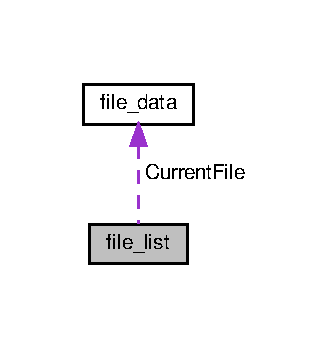
\includegraphics[width=159pt]{d8/df1/structfile__list__coll__graph}
\end{center}
\end{figure}
\subsection*{Public Attributes}
\begin{DoxyCompactItemize}
\item 
glob\+\_\+t \hyperlink{structfile__list_a8b9c52b0dbeb615a3d2ec8c4e75fce49}{Glob\+Data}
\item 
size\+\_\+t \hyperlink{structfile__list_a1f88f1b450c176c81c7ffdd7d5334429}{File\+Count}
\item 
\hyperlink{ab__common_8h_afaa62991928fb9fb18ff0db62a040aba}{u32} \hyperlink{structfile__list_a18a2bcd2708d290b02cb3a80a3f68d48}{File\+Index}
\item 
\hyperlink{structfile__data}{file\+\_\+data} $\ast$ \hyperlink{structfile__list_a8103a737b7c8edc9da8dfa5c75abe242}{Current\+File}
\item 
char \hyperlink{structfile__list_a50f2703df63faf3266542b422b417cd9}{Path} \mbox{[}\hyperlink{ab__file_8h_ab99ded389af74001a6298fc9e44e74e5}{M\+A\+X\+\_\+\+P\+A\+TH}\mbox{]}
\item 
H\+A\+N\+D\+LE \hyperlink{structfile__list_a890b377545055c3acb0d705ea20a13c4}{File\+Search\+Handle}
\item 
\hyperlink{ab__common_8h_a70e369648385b50f2d0588e8e8745275}{b8} \hyperlink{structfile__list_ab563e99003e66a0dbee5f5e4a4129b84}{is\+Dir\+Valid}
\end{DoxyCompactItemize}


\subsection{Member Data Documentation}
\mbox{\Hypertarget{structfile__list_a8103a737b7c8edc9da8dfa5c75abe242}\label{structfile__list_a8103a737b7c8edc9da8dfa5c75abe242}} 
\index{file\+\_\+list@{file\+\_\+list}!Current\+File@{Current\+File}}
\index{Current\+File@{Current\+File}!file\+\_\+list@{file\+\_\+list}}
\subsubsection{\texorpdfstring{Current\+File}{CurrentFile}}
{\footnotesize\ttfamily \hyperlink{structfile__data}{file\+\_\+data} $\ast$ file\+\_\+list\+::\+Current\+File}

\mbox{\Hypertarget{structfile__list_a1f88f1b450c176c81c7ffdd7d5334429}\label{structfile__list_a1f88f1b450c176c81c7ffdd7d5334429}} 
\index{file\+\_\+list@{file\+\_\+list}!File\+Count@{File\+Count}}
\index{File\+Count@{File\+Count}!file\+\_\+list@{file\+\_\+list}}
\subsubsection{\texorpdfstring{File\+Count}{FileCount}}
{\footnotesize\ttfamily size\+\_\+t file\+\_\+list\+::\+File\+Count}

\mbox{\Hypertarget{structfile__list_a18a2bcd2708d290b02cb3a80a3f68d48}\label{structfile__list_a18a2bcd2708d290b02cb3a80a3f68d48}} 
\index{file\+\_\+list@{file\+\_\+list}!File\+Index@{File\+Index}}
\index{File\+Index@{File\+Index}!file\+\_\+list@{file\+\_\+list}}
\subsubsection{\texorpdfstring{File\+Index}{FileIndex}}
{\footnotesize\ttfamily \hyperlink{ab__common_8h_afaa62991928fb9fb18ff0db62a040aba}{u32} file\+\_\+list\+::\+File\+Index}

\mbox{\Hypertarget{structfile__list_a890b377545055c3acb0d705ea20a13c4}\label{structfile__list_a890b377545055c3acb0d705ea20a13c4}} 
\index{file\+\_\+list@{file\+\_\+list}!File\+Search\+Handle@{File\+Search\+Handle}}
\index{File\+Search\+Handle@{File\+Search\+Handle}!file\+\_\+list@{file\+\_\+list}}
\subsubsection{\texorpdfstring{File\+Search\+Handle}{FileSearchHandle}}
{\footnotesize\ttfamily H\+A\+N\+D\+LE file\+\_\+list\+::\+File\+Search\+Handle}

\mbox{\Hypertarget{structfile__list_a8b9c52b0dbeb615a3d2ec8c4e75fce49}\label{structfile__list_a8b9c52b0dbeb615a3d2ec8c4e75fce49}} 
\index{file\+\_\+list@{file\+\_\+list}!Glob\+Data@{Glob\+Data}}
\index{Glob\+Data@{Glob\+Data}!file\+\_\+list@{file\+\_\+list}}
\subsubsection{\texorpdfstring{Glob\+Data}{GlobData}}
{\footnotesize\ttfamily glob\+\_\+t file\+\_\+list\+::\+Glob\+Data}

\mbox{\Hypertarget{structfile__list_ab563e99003e66a0dbee5f5e4a4129b84}\label{structfile__list_ab563e99003e66a0dbee5f5e4a4129b84}} 
\index{file\+\_\+list@{file\+\_\+list}!is\+Dir\+Valid@{is\+Dir\+Valid}}
\index{is\+Dir\+Valid@{is\+Dir\+Valid}!file\+\_\+list@{file\+\_\+list}}
\subsubsection{\texorpdfstring{is\+Dir\+Valid}{isDirValid}}
{\footnotesize\ttfamily \hyperlink{ab__common_8h_a70e369648385b50f2d0588e8e8745275}{b8} file\+\_\+list\+::is\+Dir\+Valid}

\mbox{\Hypertarget{structfile__list_a50f2703df63faf3266542b422b417cd9}\label{structfile__list_a50f2703df63faf3266542b422b417cd9}} 
\index{file\+\_\+list@{file\+\_\+list}!Path@{Path}}
\index{Path@{Path}!file\+\_\+list@{file\+\_\+list}}
\subsubsection{\texorpdfstring{Path}{Path}}
{\footnotesize\ttfamily char file\+\_\+list\+::\+Path}



The documentation for this struct was generated from the following files\+:\begin{DoxyCompactItemize}
\item 
\hyperlink{ab__file__linux_8h}{ab\+\_\+file\+\_\+linux.\+h}\item 
\hyperlink{ab__file__win32_8h}{ab\+\_\+file\+\_\+win32.\+h}\end{DoxyCompactItemize}

\hypertarget{structmemory__arena}{}\section{memory\+\_\+arena Struct Reference}
\label{structmemory__arena}\index{memory\+\_\+arena@{memory\+\_\+arena}}


{\ttfamily \#include $<$ab\+\_\+memory.\+h$>$}

\subsection*{Public Attributes}
\begin{DoxyCompactItemize}
\item 
void $\ast$ \hyperlink{structmemory__arena_a165e8a081bbf8241543164a8a0c580ea}{Start}
\item 
size\+\_\+t \hyperlink{structmemory__arena_ab3f96c20bd889e66879338831549af70}{Size}
\item 
size\+\_\+t \hyperlink{structmemory__arena_abbc4860a3014af6eae9d663a4e1e12d9}{Used}
\end{DoxyCompactItemize}


\subsection{Detailed Description}
======================================================================= \begin{DoxyParagraph}{File}

\end{DoxyParagraph}
\begin{DoxyParagraph}{Date}

\end{DoxyParagraph}
\begin{DoxyParagraph}{Revision}

\end{DoxyParagraph}
\begin{DoxyParagraph}{Creator}
Amos Buchanan 
\end{DoxyParagraph}
\begin{DoxyParagraph}{Email}
\href{mailto:amos.buchanan@traxxautomation.com}{\tt amos.\+buchanan@traxxautomation.\+com} 
\end{DoxyParagraph}
\subsection*{}

\subsection{Member Data Documentation}
\mbox{\Hypertarget{structmemory__arena_ab3f96c20bd889e66879338831549af70}\label{structmemory__arena_ab3f96c20bd889e66879338831549af70}} 
\index{memory\+\_\+arena@{memory\+\_\+arena}!Size@{Size}}
\index{Size@{Size}!memory\+\_\+arena@{memory\+\_\+arena}}
\subsubsection{\texorpdfstring{Size}{Size}}
{\footnotesize\ttfamily size\+\_\+t memory\+\_\+arena\+::\+Size}

\mbox{\Hypertarget{structmemory__arena_a165e8a081bbf8241543164a8a0c580ea}\label{structmemory__arena_a165e8a081bbf8241543164a8a0c580ea}} 
\index{memory\+\_\+arena@{memory\+\_\+arena}!Start@{Start}}
\index{Start@{Start}!memory\+\_\+arena@{memory\+\_\+arena}}
\subsubsection{\texorpdfstring{Start}{Start}}
{\footnotesize\ttfamily void$\ast$ memory\+\_\+arena\+::\+Start}

\mbox{\Hypertarget{structmemory__arena_abbc4860a3014af6eae9d663a4e1e12d9}\label{structmemory__arena_abbc4860a3014af6eae9d663a4e1e12d9}} 
\index{memory\+\_\+arena@{memory\+\_\+arena}!Used@{Used}}
\index{Used@{Used}!memory\+\_\+arena@{memory\+\_\+arena}}
\subsubsection{\texorpdfstring{Used}{Used}}
{\footnotesize\ttfamily size\+\_\+t memory\+\_\+arena\+::\+Used}



The documentation for this struct was generated from the following file\+:\begin{DoxyCompactItemize}
\item 
\hyperlink{ab__memory_8h}{ab\+\_\+memory.\+h}\end{DoxyCompactItemize}

\hypertarget{structtemporary__memory}{}\section{temporary\+\_\+memory Struct Reference}
\label{structtemporary__memory}\index{temporary\+\_\+memory@{temporary\+\_\+memory}}


{\ttfamily \#include $<$ab\+\_\+memory.\+h$>$}



Collaboration diagram for temporary\+\_\+memory\+:\nopagebreak
\begin{figure}[H]
\begin{center}
\leavevmode
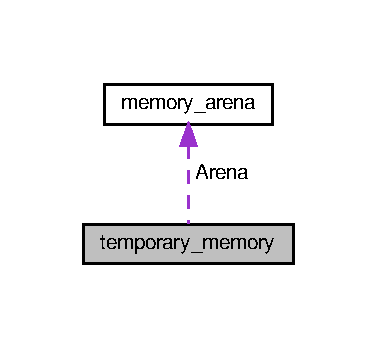
\includegraphics[width=181pt]{db/d58/structtemporary__memory__coll__graph}
\end{center}
\end{figure}
\subsection*{Public Attributes}
\begin{DoxyCompactItemize}
\item 
\hyperlink{structmemory__arena}{memory\+\_\+arena} $\ast$ \hyperlink{structtemporary__memory_abda353234998fedd47ef739e61bddeea}{Arena}
\item 
size\+\_\+t \hyperlink{structtemporary__memory_af2ea8e067d881e044fbecd269e59a556}{Used}
\end{DoxyCompactItemize}


\subsection{Member Data Documentation}
\mbox{\Hypertarget{structtemporary__memory_abda353234998fedd47ef739e61bddeea}\label{structtemporary__memory_abda353234998fedd47ef739e61bddeea}} 
\index{temporary\+\_\+memory@{temporary\+\_\+memory}!Arena@{Arena}}
\index{Arena@{Arena}!temporary\+\_\+memory@{temporary\+\_\+memory}}
\subsubsection{\texorpdfstring{Arena}{Arena}}
{\footnotesize\ttfamily \hyperlink{structmemory__arena}{memory\+\_\+arena}$\ast$ temporary\+\_\+memory\+::\+Arena}

\mbox{\Hypertarget{structtemporary__memory_af2ea8e067d881e044fbecd269e59a556}\label{structtemporary__memory_af2ea8e067d881e044fbecd269e59a556}} 
\index{temporary\+\_\+memory@{temporary\+\_\+memory}!Used@{Used}}
\index{Used@{Used}!temporary\+\_\+memory@{temporary\+\_\+memory}}
\subsubsection{\texorpdfstring{Used}{Used}}
{\footnotesize\ttfamily size\+\_\+t temporary\+\_\+memory\+::\+Used}



The documentation for this struct was generated from the following file\+:\begin{DoxyCompactItemize}
\item 
\hyperlink{ab__memory_8h}{ab\+\_\+memory.\+h}\end{DoxyCompactItemize}

\chapter{File Documentation}
\hypertarget{ab__common_8h}{}\doxysection{ab\+\_\+common.\+h File Reference}
\label{ab__common_8h}\index{ab\_common.h@{ab\_common.h}}


Common macros and typedefs.  


{\ttfamily \#include $<$stdint.\+h$>$}\newline
{\ttfamily \#include $<$wchar.\+h$>$}\newline
Include dependency graph for ab\+\_\+common.\+h\+:\nopagebreak
\begin{figure}[H]
\begin{center}
\leavevmode
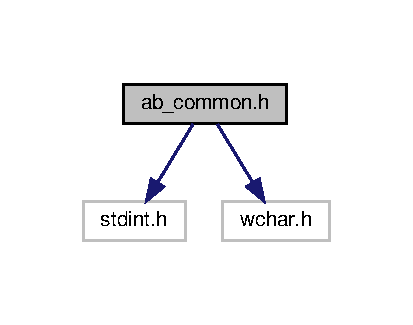
\includegraphics[width=198pt]{d1/dd0/ab__common_8h__incl}
\end{center}
\end{figure}
This graph shows which files directly or indirectly include this file\+:\nopagebreak
\begin{figure}[H]
\begin{center}
\leavevmode
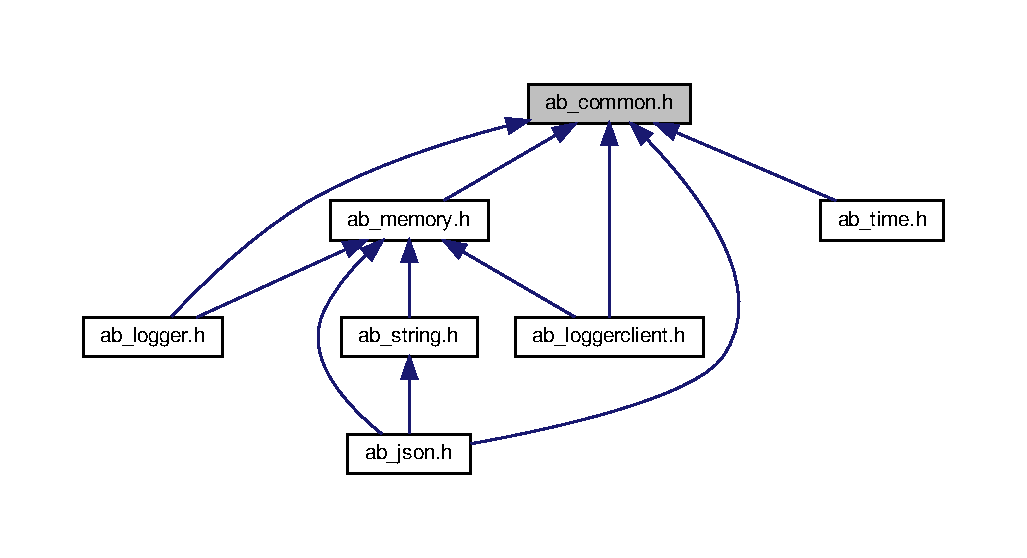
\includegraphics[width=335pt]{d8/da5/ab__common_8h__dep__incl}
\end{center}
\end{figure}
\doxysubsection*{Macros}
\begin{DoxyCompactItemize}
\item 
\#define \mbox{\hyperlink{ab__common_8h_a49450bdfb96baf39e5679e3749dd6648}{Array\+Count}}(Array)~(sizeof(Array)) / (sizeof(Array\mbox{[}0\mbox{]}))
\begin{DoxyCompactList}\small\item\em Macro that can be used anywhere with a pre-\/defined array. \end{DoxyCompactList}\item 
\#define \mbox{\hyperlink{ab__common_8h_a1da41d527b391b557b30acdc9e2cf425}{M\+A\+X\+\_\+\+F\+I\+L\+E\+N\+A\+M\+E\+\_\+\+S\+I\+ZE}}~255
\item 
\#define \mbox{\hyperlink{ab__common_8h_ab569440ccd9ea3398cfc4d514fb5493f}{M\+I\+N\+I\+M\+UM}}(Value1,  Value2)~(((Value1) $<$ (Value2)) ? (Value1) \+: (Value2))
\begin{DoxyCompactList}\small\item\em Return the minimum of a value. \end{DoxyCompactList}\item 
\#define \mbox{\hyperlink{ab__common_8h_aa0dcb9de6453c0e93a7d4c26739380e2}{M\+A\+X\+I\+M\+UM}}(Value1,  Value2)~(((Value1) $>$ (Value2)) ? (Value1) \+: (Value2))
\begin{DoxyCompactList}\small\item\em Return the maximum of a value. \end{DoxyCompactList}\item 
\#define \mbox{\hyperlink{ab__common_8h_a20bc847a34a521a2e6fa125621be9bfc}{Bit\+Reset}}(Value,  Bit)~((Value) \&= $\sim$(1 $<$$<$ (Bit)))
\begin{DoxyCompactList}\small\item\em Reset the bit to zero. \end{DoxyCompactList}\item 
\#define \mbox{\hyperlink{ab__common_8h_a1eeb0506b4ddd8d37c817456de87f052}{Bit\+Set}}(Value,  Bit)~((Value) $\vert$= (1 $<$$<$ (Bit)))
\begin{DoxyCompactList}\small\item\em Set the bit to one. \end{DoxyCompactList}\item 
\#define \mbox{\hyperlink{ab__common_8h_a9e89c74d1fedd0a954107d7ab01481cc}{Kilobytes}}(num)~(1024U\+LL $\ast$ (num))
\item 
\#define \mbox{\hyperlink{ab__common_8h_a2617ed135c31ace7205aae9398392eca}{Megabytes}}(num)~(1024U\+LL $\ast$ \mbox{\hyperlink{ab__common_8h_a9e89c74d1fedd0a954107d7ab01481cc}{Kilobytes}}(num))
\item 
\#define \mbox{\hyperlink{ab__common_8h_ae0b63ae9651c6178680d84f4900e0a0d}{Gigabytes}}(num)~(1024U\+LL $\ast$ \mbox{\hyperlink{ab__common_8h_a2617ed135c31ace7205aae9398392eca}{Megabytes}}(num))
\item 
\#define \mbox{\hyperlink{ab__common_8h_aa01ae46693c8d6cada0f39d78e8da9f8}{Terabytes}}(num)~(1024U\+LL $\ast$ \mbox{\hyperlink{ab__common_8h_ae0b63ae9651c6178680d84f4900e0a0d}{Gigabytes}}(num))
\item 
\#define \mbox{\hyperlink{ab__common_8h_a20fa811b86f3ecd1f72ae57753c26d56}{S\+\_\+\+T\+O\+\_\+\+MS}}(num)~((num) $\ast$ 1000L)
\item 
\#define \mbox{\hyperlink{ab__common_8h_ad8619bfe2bde192cdb90aaa749de313a}{S\+\_\+\+T\+O\+\_\+\+NS}}(num)~((num) $\ast$ 1e9L)
\item 
\#define \mbox{\hyperlink{ab__common_8h_af99d895a4fb9ef16b8773bfb4682cb0b}{M\+S\+\_\+\+T\+O\+\_\+S}}(num)~((num) $\ast$ 0.\+001f)
\item 
\#define \mbox{\hyperlink{ab__common_8h_a830e4dd55a9d1f281527e77f61993194}{M\+S\+\_\+\+T\+O\+\_\+\+NS}}(num)~((num) $\ast$ 1000000.\+0f)
\item 
\#define \mbox{\hyperlink{ab__common_8h_a5ea52ba9d4cb9e553e52d1c7283b58a7}{N\+S\+\_\+\+T\+O\+\_\+S}}(num)~((num) $\ast$ 1e-\/9f)
\item 
\#define \mbox{\hyperlink{ab__common_8h_a323127aaf9260b4e2092a8734886379a}{N\+S\+\_\+\+T\+O\+\_\+\+MS}}(num)~((num) $\ast$ 1e-\/6f)
\item 
\#define \mbox{\hyperlink{ab__common_8h_af2b46bb19c7d3d91950a9f971d443ccd}{Assert}}(test)
\begin{DoxyCompactList}\small\item\em Assert causes a hard-\/fault, useful when debugging. Don\textquotesingle{}t use this is production code. \end{DoxyCompactList}\end{DoxyCompactItemize}
\doxysubsection*{Typedefs}
\begin{DoxyCompactItemize}
\item 
typedef wchar\+\_\+t \mbox{\hyperlink{ab__common_8h_a59dcfa356b98a549d778585b6b0388e3}{wchar}}
\item 
typedef int8\+\_\+t \mbox{\hyperlink{ab__common_8h_a70e369648385b50f2d0588e8e8745275}{b8}}
\item 
typedef int8\+\_\+t \mbox{\hyperlink{ab__common_8h_a9e382f207c65ca13ab4ae98363aeda80}{s8}}
\item 
typedef uint8\+\_\+t \mbox{\hyperlink{ab__common_8h_a92c50087ca0e64fa93fc59402c55f8ca}{u8}}
\item 
typedef int16\+\_\+t \mbox{\hyperlink{ab__common_8h_aa980e2c02ba2305e0f489d5650655425}{s16}}
\item 
typedef uint16\+\_\+t \mbox{\hyperlink{ab__common_8h_ace9d960e74685e2cd84b36132dbbf8aa}{u16}}
\item 
typedef int32\+\_\+t \mbox{\hyperlink{ab__common_8h_ae9b1af5c037e57a98884758875d3a7c4}{s32}}
\item 
typedef uint32\+\_\+t \mbox{\hyperlink{ab__common_8h_afaa62991928fb9fb18ff0db62a040aba}{u32}}
\item 
typedef int64\+\_\+t \mbox{\hyperlink{ab__common_8h_a350c6fc928e3bdc6c6486268ac8fb269}{s64}}
\item 
typedef uint64\+\_\+t \mbox{\hyperlink{ab__common_8h_a3f7e2bcbb0b4c338f3c4f6c937cd4234}{u64}}
\item 
typedef float \mbox{\hyperlink{ab__common_8h_aafa04bc3cb166e826b75a23f4add4b59}{r32}}
\item 
typedef double \mbox{\hyperlink{ab__common_8h_af3fb0780dd5bc8ff8740028f077610e7}{r64}}
\end{DoxyCompactItemize}
\doxysubsection*{Variables}
\begin{DoxyCompactItemize}
\item 
const \mbox{\hyperlink{ab__common_8h_aafa04bc3cb166e826b75a23f4add4b59}{r32}} \mbox{\hyperlink{ab__common_8h_a680f0d86b7fc8e450b05875fc7e2cee7}{T\+AU}} = 6.\+2831853071f
\end{DoxyCompactItemize}


\doxysubsection{Detailed Description}
Common macros and typedefs. 

\begin{DoxyAuthor}{Author}
Amos Buchanan 
\end{DoxyAuthor}
\begin{DoxyVersion}{Version}
1.\+0 
\end{DoxyVersion}
\begin{DoxyDate}{Date}
2020 
\end{DoxyDate}
\begin{DoxyCopyright}{Copyright}
\href{https://opensource.org/licenses/MIT}{\texttt{ M\+IT Public License}}
\end{DoxyCopyright}
This file has the common macros and typedefs I use everywhere. Every other library is dependent on this one.

\doxysubsection*{M\+IT License}

\href{https://opensource.org/licenses/MIT}{\texttt{ M\+IT Public License}}

Copyright 2020 Amos Buchanan

Permission is hereby granted, free of charge, to any person obtaining a copy of this software and associated documentation files (the \char`\"{}\+Software\char`\"{}), to deal in the Software without restriction, including without limitation the rights to use, copy, modify, merge, publish, distribute, sublicense, and/or sell copies of the Software, and to permit persons to whom the Software is furnished to do so, subject to the following conditions\+:

The above copyright notice and this permission notice shall be included in all copies or substantial portions of the Software.

T\+HE S\+O\+F\+T\+W\+A\+RE IS P\+R\+O\+V\+I\+D\+ED \char`\"{}\+A\+S I\+S\char`\"{}, W\+I\+T\+H\+O\+UT W\+A\+R\+R\+A\+N\+TY OF A\+NY K\+I\+ND, E\+X\+P\+R\+E\+SS OR I\+M\+P\+L\+I\+ED, I\+N\+C\+L\+U\+D\+I\+NG B\+UT N\+OT L\+I\+M\+I\+T\+ED TO T\+HE W\+A\+R\+R\+A\+N\+T\+I\+ES OF M\+E\+R\+C\+H\+A\+N\+T\+A\+B\+I\+L\+I\+TY, F\+I\+T\+N\+E\+SS F\+OR A P\+A\+R\+T\+I\+C\+U\+L\+AR P\+U\+R\+P\+O\+SE A\+ND N\+O\+N\+I\+N\+F\+R\+I\+N\+G\+E\+M\+E\+NT. IN NO E\+V\+E\+NT S\+H\+A\+LL T\+HE A\+U\+T\+H\+O\+RS OR C\+O\+P\+Y\+R\+I\+G\+HT H\+O\+L\+D\+E\+RS BE L\+I\+A\+B\+LE F\+OR A\+NY C\+L\+A\+IM, D\+A\+M\+A\+G\+ES OR O\+T\+H\+ER L\+I\+A\+B\+I\+L\+I\+TY, W\+H\+E\+T\+H\+ER IN AN A\+C\+T\+I\+ON OF C\+O\+N\+T\+R\+A\+CT, T\+O\+RT OR O\+T\+H\+E\+R\+W\+I\+SE, A\+R\+I\+S\+I\+NG F\+R\+OM, O\+UT OF OR IN C\+O\+N\+N\+E\+C\+T\+I\+ON W\+I\+TH T\+HE S\+O\+F\+T\+W\+A\+RE OR T\+HE U\+SE OR O\+T\+H\+ER D\+E\+A\+L\+I\+N\+GS IN T\+HE S\+O\+F\+T\+W\+A\+RE. 

\doxysubsection{Macro Definition Documentation}
\mbox{\Hypertarget{ab__common_8h_a49450bdfb96baf39e5679e3749dd6648}\label{ab__common_8h_a49450bdfb96baf39e5679e3749dd6648}} 
\index{ab\_common.h@{ab\_common.h}!ArrayCount@{ArrayCount}}
\index{ArrayCount@{ArrayCount}!ab\_common.h@{ab\_common.h}}
\doxysubsubsection{\texorpdfstring{ArrayCount}{ArrayCount}}
{\footnotesize\ttfamily \#define Array\+Count(\begin{DoxyParamCaption}\item[{}]{Array }\end{DoxyParamCaption})~(sizeof(Array)) / (sizeof(Array\mbox{[}0\mbox{]}))}



Macro that can be used anywhere with a pre-\/defined array. 

\mbox{\Hypertarget{ab__common_8h_af2b46bb19c7d3d91950a9f971d443ccd}\label{ab__common_8h_af2b46bb19c7d3d91950a9f971d443ccd}} 
\index{ab\_common.h@{ab\_common.h}!Assert@{Assert}}
\index{Assert@{Assert}!ab\_common.h@{ab\_common.h}}
\doxysubsubsection{\texorpdfstring{Assert}{Assert}}
{\footnotesize\ttfamily \#define Assert(\begin{DoxyParamCaption}\item[{}]{test }\end{DoxyParamCaption})}



Assert causes a hard-\/fault, useful when debugging. Don\textquotesingle{}t use this is production code. 

\mbox{\Hypertarget{ab__common_8h_a20bc847a34a521a2e6fa125621be9bfc}\label{ab__common_8h_a20bc847a34a521a2e6fa125621be9bfc}} 
\index{ab\_common.h@{ab\_common.h}!BitReset@{BitReset}}
\index{BitReset@{BitReset}!ab\_common.h@{ab\_common.h}}
\doxysubsubsection{\texorpdfstring{BitReset}{BitReset}}
{\footnotesize\ttfamily \#define Bit\+Reset(\begin{DoxyParamCaption}\item[{}]{Value,  }\item[{}]{Bit }\end{DoxyParamCaption})~((Value) \&= $\sim$(1 $<$$<$ (Bit)))}



Reset the bit to zero. 

\mbox{\Hypertarget{ab__common_8h_a1eeb0506b4ddd8d37c817456de87f052}\label{ab__common_8h_a1eeb0506b4ddd8d37c817456de87f052}} 
\index{ab\_common.h@{ab\_common.h}!BitSet@{BitSet}}
\index{BitSet@{BitSet}!ab\_common.h@{ab\_common.h}}
\doxysubsubsection{\texorpdfstring{BitSet}{BitSet}}
{\footnotesize\ttfamily \#define Bit\+Set(\begin{DoxyParamCaption}\item[{}]{Value,  }\item[{}]{Bit }\end{DoxyParamCaption})~((Value) $\vert$= (1 $<$$<$ (Bit)))}



Set the bit to one. 

\mbox{\Hypertarget{ab__common_8h_ae0b63ae9651c6178680d84f4900e0a0d}\label{ab__common_8h_ae0b63ae9651c6178680d84f4900e0a0d}} 
\index{ab\_common.h@{ab\_common.h}!Gigabytes@{Gigabytes}}
\index{Gigabytes@{Gigabytes}!ab\_common.h@{ab\_common.h}}
\doxysubsubsection{\texorpdfstring{Gigabytes}{Gigabytes}}
{\footnotesize\ttfamily \#define Gigabytes(\begin{DoxyParamCaption}\item[{}]{num }\end{DoxyParamCaption})~(1024U\+LL $\ast$ \mbox{\hyperlink{ab__common_8h_a2617ed135c31ace7205aae9398392eca}{Megabytes}}(num))}

\mbox{\Hypertarget{ab__common_8h_a9e89c74d1fedd0a954107d7ab01481cc}\label{ab__common_8h_a9e89c74d1fedd0a954107d7ab01481cc}} 
\index{ab\_common.h@{ab\_common.h}!Kilobytes@{Kilobytes}}
\index{Kilobytes@{Kilobytes}!ab\_common.h@{ab\_common.h}}
\doxysubsubsection{\texorpdfstring{Kilobytes}{Kilobytes}}
{\footnotesize\ttfamily \#define Kilobytes(\begin{DoxyParamCaption}\item[{}]{num }\end{DoxyParamCaption})~(1024U\+LL $\ast$ (num))}

\mbox{\Hypertarget{ab__common_8h_a1da41d527b391b557b30acdc9e2cf425}\label{ab__common_8h_a1da41d527b391b557b30acdc9e2cf425}} 
\index{ab\_common.h@{ab\_common.h}!MAX\_FILENAME\_SIZE@{MAX\_FILENAME\_SIZE}}
\index{MAX\_FILENAME\_SIZE@{MAX\_FILENAME\_SIZE}!ab\_common.h@{ab\_common.h}}
\doxysubsubsection{\texorpdfstring{MAX\_FILENAME\_SIZE}{MAX\_FILENAME\_SIZE}}
{\footnotesize\ttfamily \#define M\+A\+X\+\_\+\+F\+I\+L\+E\+N\+A\+M\+E\+\_\+\+S\+I\+ZE~255}

\mbox{\Hypertarget{ab__common_8h_aa0dcb9de6453c0e93a7d4c26739380e2}\label{ab__common_8h_aa0dcb9de6453c0e93a7d4c26739380e2}} 
\index{ab\_common.h@{ab\_common.h}!MAXIMUM@{MAXIMUM}}
\index{MAXIMUM@{MAXIMUM}!ab\_common.h@{ab\_common.h}}
\doxysubsubsection{\texorpdfstring{MAXIMUM}{MAXIMUM}}
{\footnotesize\ttfamily \#define M\+A\+X\+I\+M\+UM(\begin{DoxyParamCaption}\item[{}]{Value1,  }\item[{}]{Value2 }\end{DoxyParamCaption})~(((Value1) $>$ (Value2)) ? (Value1) \+: (Value2))}



Return the maximum of a value. 

\mbox{\Hypertarget{ab__common_8h_a2617ed135c31ace7205aae9398392eca}\label{ab__common_8h_a2617ed135c31ace7205aae9398392eca}} 
\index{ab\_common.h@{ab\_common.h}!Megabytes@{Megabytes}}
\index{Megabytes@{Megabytes}!ab\_common.h@{ab\_common.h}}
\doxysubsubsection{\texorpdfstring{Megabytes}{Megabytes}}
{\footnotesize\ttfamily \#define Megabytes(\begin{DoxyParamCaption}\item[{}]{num }\end{DoxyParamCaption})~(1024U\+LL $\ast$ \mbox{\hyperlink{ab__common_8h_a9e89c74d1fedd0a954107d7ab01481cc}{Kilobytes}}(num))}

\mbox{\Hypertarget{ab__common_8h_ab569440ccd9ea3398cfc4d514fb5493f}\label{ab__common_8h_ab569440ccd9ea3398cfc4d514fb5493f}} 
\index{ab\_common.h@{ab\_common.h}!MINIMUM@{MINIMUM}}
\index{MINIMUM@{MINIMUM}!ab\_common.h@{ab\_common.h}}
\doxysubsubsection{\texorpdfstring{MINIMUM}{MINIMUM}}
{\footnotesize\ttfamily \#define M\+I\+N\+I\+M\+UM(\begin{DoxyParamCaption}\item[{}]{Value1,  }\item[{}]{Value2 }\end{DoxyParamCaption})~(((Value1) $<$ (Value2)) ? (Value1) \+: (Value2))}



Return the minimum of a value. 

\mbox{\Hypertarget{ab__common_8h_a830e4dd55a9d1f281527e77f61993194}\label{ab__common_8h_a830e4dd55a9d1f281527e77f61993194}} 
\index{ab\_common.h@{ab\_common.h}!MS\_TO\_NS@{MS\_TO\_NS}}
\index{MS\_TO\_NS@{MS\_TO\_NS}!ab\_common.h@{ab\_common.h}}
\doxysubsubsection{\texorpdfstring{MS\_TO\_NS}{MS\_TO\_NS}}
{\footnotesize\ttfamily \#define M\+S\+\_\+\+T\+O\+\_\+\+NS(\begin{DoxyParamCaption}\item[{}]{num }\end{DoxyParamCaption})~((num) $\ast$ 1000000.\+0f)}

\mbox{\Hypertarget{ab__common_8h_af99d895a4fb9ef16b8773bfb4682cb0b}\label{ab__common_8h_af99d895a4fb9ef16b8773bfb4682cb0b}} 
\index{ab\_common.h@{ab\_common.h}!MS\_TO\_S@{MS\_TO\_S}}
\index{MS\_TO\_S@{MS\_TO\_S}!ab\_common.h@{ab\_common.h}}
\doxysubsubsection{\texorpdfstring{MS\_TO\_S}{MS\_TO\_S}}
{\footnotesize\ttfamily \#define M\+S\+\_\+\+T\+O\+\_\+S(\begin{DoxyParamCaption}\item[{}]{num }\end{DoxyParamCaption})~((num) $\ast$ 0.\+001f)}

\mbox{\Hypertarget{ab__common_8h_a323127aaf9260b4e2092a8734886379a}\label{ab__common_8h_a323127aaf9260b4e2092a8734886379a}} 
\index{ab\_common.h@{ab\_common.h}!NS\_TO\_MS@{NS\_TO\_MS}}
\index{NS\_TO\_MS@{NS\_TO\_MS}!ab\_common.h@{ab\_common.h}}
\doxysubsubsection{\texorpdfstring{NS\_TO\_MS}{NS\_TO\_MS}}
{\footnotesize\ttfamily \#define N\+S\+\_\+\+T\+O\+\_\+\+MS(\begin{DoxyParamCaption}\item[{}]{num }\end{DoxyParamCaption})~((num) $\ast$ 1e-\/6f)}

\mbox{\Hypertarget{ab__common_8h_a5ea52ba9d4cb9e553e52d1c7283b58a7}\label{ab__common_8h_a5ea52ba9d4cb9e553e52d1c7283b58a7}} 
\index{ab\_common.h@{ab\_common.h}!NS\_TO\_S@{NS\_TO\_S}}
\index{NS\_TO\_S@{NS\_TO\_S}!ab\_common.h@{ab\_common.h}}
\doxysubsubsection{\texorpdfstring{NS\_TO\_S}{NS\_TO\_S}}
{\footnotesize\ttfamily \#define N\+S\+\_\+\+T\+O\+\_\+S(\begin{DoxyParamCaption}\item[{}]{num }\end{DoxyParamCaption})~((num) $\ast$ 1e-\/9f)}

\mbox{\Hypertarget{ab__common_8h_a20fa811b86f3ecd1f72ae57753c26d56}\label{ab__common_8h_a20fa811b86f3ecd1f72ae57753c26d56}} 
\index{ab\_common.h@{ab\_common.h}!S\_TO\_MS@{S\_TO\_MS}}
\index{S\_TO\_MS@{S\_TO\_MS}!ab\_common.h@{ab\_common.h}}
\doxysubsubsection{\texorpdfstring{S\_TO\_MS}{S\_TO\_MS}}
{\footnotesize\ttfamily \#define S\+\_\+\+T\+O\+\_\+\+MS(\begin{DoxyParamCaption}\item[{}]{num }\end{DoxyParamCaption})~((num) $\ast$ 1000L)}

\mbox{\Hypertarget{ab__common_8h_ad8619bfe2bde192cdb90aaa749de313a}\label{ab__common_8h_ad8619bfe2bde192cdb90aaa749de313a}} 
\index{ab\_common.h@{ab\_common.h}!S\_TO\_NS@{S\_TO\_NS}}
\index{S\_TO\_NS@{S\_TO\_NS}!ab\_common.h@{ab\_common.h}}
\doxysubsubsection{\texorpdfstring{S\_TO\_NS}{S\_TO\_NS}}
{\footnotesize\ttfamily \#define S\+\_\+\+T\+O\+\_\+\+NS(\begin{DoxyParamCaption}\item[{}]{num }\end{DoxyParamCaption})~((num) $\ast$ 1e9L)}

\mbox{\Hypertarget{ab__common_8h_aa01ae46693c8d6cada0f39d78e8da9f8}\label{ab__common_8h_aa01ae46693c8d6cada0f39d78e8da9f8}} 
\index{ab\_common.h@{ab\_common.h}!Terabytes@{Terabytes}}
\index{Terabytes@{Terabytes}!ab\_common.h@{ab\_common.h}}
\doxysubsubsection{\texorpdfstring{Terabytes}{Terabytes}}
{\footnotesize\ttfamily \#define Terabytes(\begin{DoxyParamCaption}\item[{}]{num }\end{DoxyParamCaption})~(1024U\+LL $\ast$ \mbox{\hyperlink{ab__common_8h_ae0b63ae9651c6178680d84f4900e0a0d}{Gigabytes}}(num))}



\doxysubsection{Typedef Documentation}
\mbox{\Hypertarget{ab__common_8h_a70e369648385b50f2d0588e8e8745275}\label{ab__common_8h_a70e369648385b50f2d0588e8e8745275}} 
\index{ab\_common.h@{ab\_common.h}!b8@{b8}}
\index{b8@{b8}!ab\_common.h@{ab\_common.h}}
\doxysubsubsection{\texorpdfstring{b8}{b8}}
{\footnotesize\ttfamily typedef int8\+\_\+t \mbox{\hyperlink{ab__common_8h_a70e369648385b50f2d0588e8e8745275}{b8}}}

\mbox{\Hypertarget{ab__common_8h_aafa04bc3cb166e826b75a23f4add4b59}\label{ab__common_8h_aafa04bc3cb166e826b75a23f4add4b59}} 
\index{ab\_common.h@{ab\_common.h}!r32@{r32}}
\index{r32@{r32}!ab\_common.h@{ab\_common.h}}
\doxysubsubsection{\texorpdfstring{r32}{r32}}
{\footnotesize\ttfamily typedef float \mbox{\hyperlink{ab__common_8h_aafa04bc3cb166e826b75a23f4add4b59}{r32}}}

\mbox{\Hypertarget{ab__common_8h_af3fb0780dd5bc8ff8740028f077610e7}\label{ab__common_8h_af3fb0780dd5bc8ff8740028f077610e7}} 
\index{ab\_common.h@{ab\_common.h}!r64@{r64}}
\index{r64@{r64}!ab\_common.h@{ab\_common.h}}
\doxysubsubsection{\texorpdfstring{r64}{r64}}
{\footnotesize\ttfamily typedef double \mbox{\hyperlink{ab__common_8h_af3fb0780dd5bc8ff8740028f077610e7}{r64}}}

\mbox{\Hypertarget{ab__common_8h_aa980e2c02ba2305e0f489d5650655425}\label{ab__common_8h_aa980e2c02ba2305e0f489d5650655425}} 
\index{ab\_common.h@{ab\_common.h}!s16@{s16}}
\index{s16@{s16}!ab\_common.h@{ab\_common.h}}
\doxysubsubsection{\texorpdfstring{s16}{s16}}
{\footnotesize\ttfamily typedef int16\+\_\+t \mbox{\hyperlink{ab__common_8h_aa980e2c02ba2305e0f489d5650655425}{s16}}}

\mbox{\Hypertarget{ab__common_8h_ae9b1af5c037e57a98884758875d3a7c4}\label{ab__common_8h_ae9b1af5c037e57a98884758875d3a7c4}} 
\index{ab\_common.h@{ab\_common.h}!s32@{s32}}
\index{s32@{s32}!ab\_common.h@{ab\_common.h}}
\doxysubsubsection{\texorpdfstring{s32}{s32}}
{\footnotesize\ttfamily typedef int32\+\_\+t \mbox{\hyperlink{ab__common_8h_ae9b1af5c037e57a98884758875d3a7c4}{s32}}}

\mbox{\Hypertarget{ab__common_8h_a350c6fc928e3bdc6c6486268ac8fb269}\label{ab__common_8h_a350c6fc928e3bdc6c6486268ac8fb269}} 
\index{ab\_common.h@{ab\_common.h}!s64@{s64}}
\index{s64@{s64}!ab\_common.h@{ab\_common.h}}
\doxysubsubsection{\texorpdfstring{s64}{s64}}
{\footnotesize\ttfamily typedef int64\+\_\+t \mbox{\hyperlink{ab__common_8h_a350c6fc928e3bdc6c6486268ac8fb269}{s64}}}

\mbox{\Hypertarget{ab__common_8h_a9e382f207c65ca13ab4ae98363aeda80}\label{ab__common_8h_a9e382f207c65ca13ab4ae98363aeda80}} 
\index{ab\_common.h@{ab\_common.h}!s8@{s8}}
\index{s8@{s8}!ab\_common.h@{ab\_common.h}}
\doxysubsubsection{\texorpdfstring{s8}{s8}}
{\footnotesize\ttfamily typedef int8\+\_\+t \mbox{\hyperlink{ab__common_8h_a9e382f207c65ca13ab4ae98363aeda80}{s8}}}

\mbox{\Hypertarget{ab__common_8h_ace9d960e74685e2cd84b36132dbbf8aa}\label{ab__common_8h_ace9d960e74685e2cd84b36132dbbf8aa}} 
\index{ab\_common.h@{ab\_common.h}!u16@{u16}}
\index{u16@{u16}!ab\_common.h@{ab\_common.h}}
\doxysubsubsection{\texorpdfstring{u16}{u16}}
{\footnotesize\ttfamily typedef uint16\+\_\+t \mbox{\hyperlink{ab__common_8h_ace9d960e74685e2cd84b36132dbbf8aa}{u16}}}

\mbox{\Hypertarget{ab__common_8h_afaa62991928fb9fb18ff0db62a040aba}\label{ab__common_8h_afaa62991928fb9fb18ff0db62a040aba}} 
\index{ab\_common.h@{ab\_common.h}!u32@{u32}}
\index{u32@{u32}!ab\_common.h@{ab\_common.h}}
\doxysubsubsection{\texorpdfstring{u32}{u32}}
{\footnotesize\ttfamily typedef uint32\+\_\+t \mbox{\hyperlink{ab__common_8h_afaa62991928fb9fb18ff0db62a040aba}{u32}}}

\mbox{\Hypertarget{ab__common_8h_a3f7e2bcbb0b4c338f3c4f6c937cd4234}\label{ab__common_8h_a3f7e2bcbb0b4c338f3c4f6c937cd4234}} 
\index{ab\_common.h@{ab\_common.h}!u64@{u64}}
\index{u64@{u64}!ab\_common.h@{ab\_common.h}}
\doxysubsubsection{\texorpdfstring{u64}{u64}}
{\footnotesize\ttfamily typedef uint64\+\_\+t \mbox{\hyperlink{ab__common_8h_a3f7e2bcbb0b4c338f3c4f6c937cd4234}{u64}}}

\mbox{\Hypertarget{ab__common_8h_a92c50087ca0e64fa93fc59402c55f8ca}\label{ab__common_8h_a92c50087ca0e64fa93fc59402c55f8ca}} 
\index{ab\_common.h@{ab\_common.h}!u8@{u8}}
\index{u8@{u8}!ab\_common.h@{ab\_common.h}}
\doxysubsubsection{\texorpdfstring{u8}{u8}}
{\footnotesize\ttfamily typedef uint8\+\_\+t \mbox{\hyperlink{ab__common_8h_a92c50087ca0e64fa93fc59402c55f8ca}{u8}}}

\mbox{\Hypertarget{ab__common_8h_a59dcfa356b98a549d778585b6b0388e3}\label{ab__common_8h_a59dcfa356b98a549d778585b6b0388e3}} 
\index{ab\_common.h@{ab\_common.h}!wchar@{wchar}}
\index{wchar@{wchar}!ab\_common.h@{ab\_common.h}}
\doxysubsubsection{\texorpdfstring{wchar}{wchar}}
{\footnotesize\ttfamily typedef wchar\+\_\+t \mbox{\hyperlink{ab__common_8h_a59dcfa356b98a549d778585b6b0388e3}{wchar}}}



\doxysubsection{Variable Documentation}
\mbox{\Hypertarget{ab__common_8h_a680f0d86b7fc8e450b05875fc7e2cee7}\label{ab__common_8h_a680f0d86b7fc8e450b05875fc7e2cee7}} 
\index{ab\_common.h@{ab\_common.h}!TAU@{TAU}}
\index{TAU@{TAU}!ab\_common.h@{ab\_common.h}}
\doxysubsubsection{\texorpdfstring{TAU}{TAU}}
{\footnotesize\ttfamily const \mbox{\hyperlink{ab__common_8h_aafa04bc3cb166e826b75a23f4add4b59}{r32}} T\+AU = 6.\+2831853071f}


\hypertarget{ab__file_8h}{}\section{ab\+\_\+file.\+h File Reference}
\label{ab__file_8h}\index{ab\+\_\+file.\+h@{ab\+\_\+file.\+h}}
{\ttfamily \#include $<$sys/stat.\+h$>$}\newline
{\ttfamily \#include \char`\"{}stb\+\_\+sprintf.\+h\char`\"{}}\newline
{\ttfamily \#include \char`\"{}ab\+\_\+memory.\+h\char`\"{}}\newline
Include dependency graph for ab\+\_\+file.\+h\+:\nopagebreak
\begin{figure}[H]
\begin{center}
\leavevmode
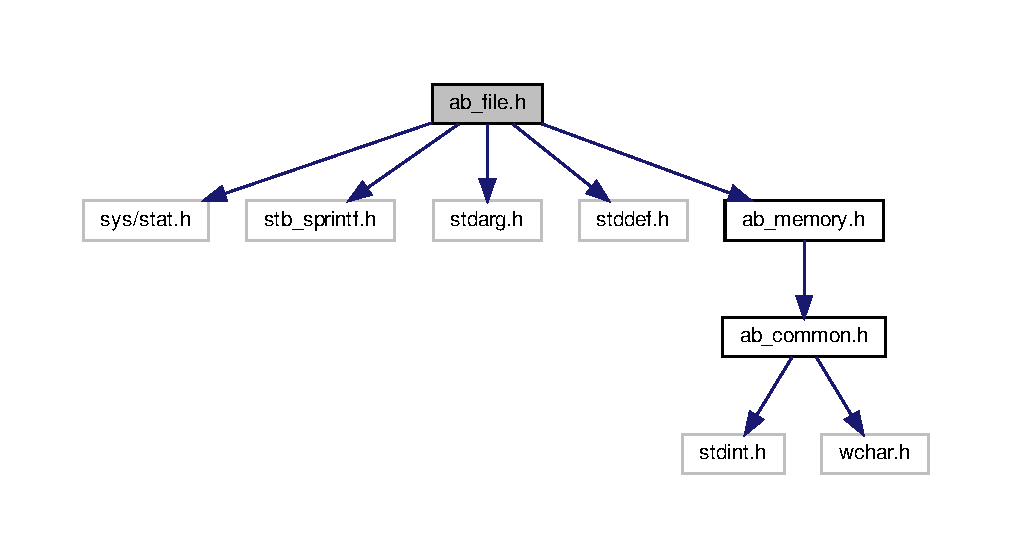
\includegraphics[width=350pt]{df/d58/ab__file_8h__incl}
\end{center}
\end{figure}
\subsection*{Classes}
\begin{DoxyCompactItemize}
\item 
struct \hyperlink{structfile__data}{file\+\_\+data}
\end{DoxyCompactItemize}
\subsection*{Macros}
\begin{DoxyCompactItemize}
\item 
\#define \hyperlink{ab__file_8h_ab99ded389af74001a6298fc9e44e74e5}{M\+A\+X\+\_\+\+P\+A\+TH}~255
\end{DoxyCompactItemize}
\subsection*{Enumerations}
\begin{DoxyCompactItemize}
\item 
enum \hyperlink{ab__file_8h_a1b665fc63cb310d53283fbcd1b19746e}{en\+File\+Type} \{ \hyperlink{ab__file_8h_a1b665fc63cb310d53283fbcd1b19746ea88183b946cc5f0e8c96b2e66e1c74a7e}{en\+File\+Type\+::\+Unknown}, 
\hyperlink{ab__file_8h_a1b665fc63cb310d53283fbcd1b19746eabf50d5e661106d0abe925af3c2e6f7e7}{en\+File\+Type\+::\+Header}, 
\hyperlink{ab__file_8h_a1b665fc63cb310d53283fbcd1b19746eadb4a39bf594c9fbcf318dd39ea19fed3}{en\+File\+Type\+::\+Cpp}
 \}
\end{DoxyCompactItemize}
\subsection*{Functions}
\begin{DoxyCompactItemize}
\item 
\hyperlink{ab__common_8h_a70e369648385b50f2d0588e8e8745275}{b8} \hyperlink{ab__file_8h_a4421ce1243877d8cc9082aae558db83f}{is\+Dir\+Exists} (const char $\ast$const path)
\item 
\hyperlink{structfile__list}{file\+\_\+list} $\ast$ \hyperlink{ab__file_8h_a3651116b0e04d2fdaedbe1154c22a46e}{abf\+\_\+\+Initialize\+File\+List} (\hyperlink{structmemory__arena}{memory\+\_\+arena} $\ast$Memory, const char $\ast$Path)
\item 
\hyperlink{ab__common_8h_a70e369648385b50f2d0588e8e8745275}{b8} \hyperlink{ab__file_8h_afba97cbbbebbd2066d87792952d894be}{abf\+\_\+\+Get\+Next\+File} (\hyperlink{structfile__list}{file\+\_\+list} $\ast$File\+List, \hyperlink{structfile__data}{file\+\_\+data} $\ast$File\+Data\+Out)
\item 
void \hyperlink{ab__file_8h_a4e85548dcb79723a8c6f468cf776826d}{abf\+\_\+\+Release\+File\+List} (\hyperlink{structfile__list}{file\+\_\+list} $\ast$File\+List)
\end{DoxyCompactItemize}


\subsection{Macro Definition Documentation}
\mbox{\Hypertarget{ab__file_8h_ab99ded389af74001a6298fc9e44e74e5}\label{ab__file_8h_ab99ded389af74001a6298fc9e44e74e5}} 
\index{ab\+\_\+file.\+h@{ab\+\_\+file.\+h}!M\+A\+X\+\_\+\+P\+A\+TH@{M\+A\+X\+\_\+\+P\+A\+TH}}
\index{M\+A\+X\+\_\+\+P\+A\+TH@{M\+A\+X\+\_\+\+P\+A\+TH}!ab\+\_\+file.\+h@{ab\+\_\+file.\+h}}
\subsubsection{\texorpdfstring{M\+A\+X\+\_\+\+P\+A\+TH}{MAX\_PATH}}
{\footnotesize\ttfamily \#define M\+A\+X\+\_\+\+P\+A\+TH~255}



\subsection{Enumeration Type Documentation}
\mbox{\Hypertarget{ab__file_8h_a1b665fc63cb310d53283fbcd1b19746e}\label{ab__file_8h_a1b665fc63cb310d53283fbcd1b19746e}} 
\index{ab\+\_\+file.\+h@{ab\+\_\+file.\+h}!en\+File\+Type@{en\+File\+Type}}
\index{en\+File\+Type@{en\+File\+Type}!ab\+\_\+file.\+h@{ab\+\_\+file.\+h}}
\subsubsection{\texorpdfstring{en\+File\+Type}{enFileType}}
{\footnotesize\ttfamily enum \hyperlink{ab__file_8h_a1b665fc63cb310d53283fbcd1b19746e}{en\+File\+Type}\hspace{0.3cm}{\ttfamily [strong]}}

\begin{DoxyEnumFields}{Enumerator}
\raisebox{\heightof{T}}[0pt][0pt]{\index{Unknown@{Unknown}!ab\+\_\+file.\+h@{ab\+\_\+file.\+h}}\index{ab\+\_\+file.\+h@{ab\+\_\+file.\+h}!Unknown@{Unknown}}}\mbox{\Hypertarget{ab__file_8h_a1b665fc63cb310d53283fbcd1b19746ea88183b946cc5f0e8c96b2e66e1c74a7e}\label{ab__file_8h_a1b665fc63cb310d53283fbcd1b19746ea88183b946cc5f0e8c96b2e66e1c74a7e}} 
Unknown&\\
\hline

\raisebox{\heightof{T}}[0pt][0pt]{\index{Header@{Header}!ab\+\_\+file.\+h@{ab\+\_\+file.\+h}}\index{ab\+\_\+file.\+h@{ab\+\_\+file.\+h}!Header@{Header}}}\mbox{\Hypertarget{ab__file_8h_a1b665fc63cb310d53283fbcd1b19746eabf50d5e661106d0abe925af3c2e6f7e7}\label{ab__file_8h_a1b665fc63cb310d53283fbcd1b19746eabf50d5e661106d0abe925af3c2e6f7e7}} 
Header&\\
\hline

\raisebox{\heightof{T}}[0pt][0pt]{\index{Cpp@{Cpp}!ab\+\_\+file.\+h@{ab\+\_\+file.\+h}}\index{ab\+\_\+file.\+h@{ab\+\_\+file.\+h}!Cpp@{Cpp}}}\mbox{\Hypertarget{ab__file_8h_a1b665fc63cb310d53283fbcd1b19746eadb4a39bf594c9fbcf318dd39ea19fed3}\label{ab__file_8h_a1b665fc63cb310d53283fbcd1b19746eadb4a39bf594c9fbcf318dd39ea19fed3}} 
Cpp&\\
\hline

\end{DoxyEnumFields}


\subsection{Function Documentation}
\mbox{\Hypertarget{ab__file_8h_afba97cbbbebbd2066d87792952d894be}\label{ab__file_8h_afba97cbbbebbd2066d87792952d894be}} 
\index{ab\+\_\+file.\+h@{ab\+\_\+file.\+h}!abf\+\_\+\+Get\+Next\+File@{abf\+\_\+\+Get\+Next\+File}}
\index{abf\+\_\+\+Get\+Next\+File@{abf\+\_\+\+Get\+Next\+File}!ab\+\_\+file.\+h@{ab\+\_\+file.\+h}}
\subsubsection{\texorpdfstring{abf\+\_\+\+Get\+Next\+File()}{abf\_GetNextFile()}}
{\footnotesize\ttfamily \hyperlink{ab__common_8h_a70e369648385b50f2d0588e8e8745275}{b8} abf\+\_\+\+Get\+Next\+File (\begin{DoxyParamCaption}\item[{\hyperlink{structfile__list}{file\+\_\+list} $\ast$}]{File\+List,  }\item[{\hyperlink{structfile__data}{file\+\_\+data} $\ast$}]{File\+Data\+Out }\end{DoxyParamCaption})}

\mbox{\Hypertarget{ab__file_8h_a3651116b0e04d2fdaedbe1154c22a46e}\label{ab__file_8h_a3651116b0e04d2fdaedbe1154c22a46e}} 
\index{ab\+\_\+file.\+h@{ab\+\_\+file.\+h}!abf\+\_\+\+Initialize\+File\+List@{abf\+\_\+\+Initialize\+File\+List}}
\index{abf\+\_\+\+Initialize\+File\+List@{abf\+\_\+\+Initialize\+File\+List}!ab\+\_\+file.\+h@{ab\+\_\+file.\+h}}
\subsubsection{\texorpdfstring{abf\+\_\+\+Initialize\+File\+List()}{abf\_InitializeFileList()}}
{\footnotesize\ttfamily \hyperlink{structfile__list}{file\+\_\+list}$\ast$ abf\+\_\+\+Initialize\+File\+List (\begin{DoxyParamCaption}\item[{\hyperlink{structmemory__arena}{memory\+\_\+arena} $\ast$}]{Memory,  }\item[{const char $\ast$}]{Path }\end{DoxyParamCaption})}

\mbox{\Hypertarget{ab__file_8h_a4e85548dcb79723a8c6f468cf776826d}\label{ab__file_8h_a4e85548dcb79723a8c6f468cf776826d}} 
\index{ab\+\_\+file.\+h@{ab\+\_\+file.\+h}!abf\+\_\+\+Release\+File\+List@{abf\+\_\+\+Release\+File\+List}}
\index{abf\+\_\+\+Release\+File\+List@{abf\+\_\+\+Release\+File\+List}!ab\+\_\+file.\+h@{ab\+\_\+file.\+h}}
\subsubsection{\texorpdfstring{abf\+\_\+\+Release\+File\+List()}{abf\_ReleaseFileList()}}
{\footnotesize\ttfamily void abf\+\_\+\+Release\+File\+List (\begin{DoxyParamCaption}\item[{\hyperlink{structfile__list}{file\+\_\+list} $\ast$}]{File\+List }\end{DoxyParamCaption})}

\mbox{\Hypertarget{ab__file_8h_a4421ce1243877d8cc9082aae558db83f}\label{ab__file_8h_a4421ce1243877d8cc9082aae558db83f}} 
\index{ab\+\_\+file.\+h@{ab\+\_\+file.\+h}!is\+Dir\+Exists@{is\+Dir\+Exists}}
\index{is\+Dir\+Exists@{is\+Dir\+Exists}!ab\+\_\+file.\+h@{ab\+\_\+file.\+h}}
\subsubsection{\texorpdfstring{is\+Dir\+Exists()}{isDirExists()}}
{\footnotesize\ttfamily \hyperlink{ab__common_8h_a70e369648385b50f2d0588e8e8745275}{b8} is\+Dir\+Exists (\begin{DoxyParamCaption}\item[{const char $\ast$const}]{path }\end{DoxyParamCaption})}


\hypertarget{ab__file__linux_8h}{}\doxysection{ab\+\_\+file\+\_\+linux.\+h File Reference}
\label{ab__file__linux_8h}\index{ab\_file\_linux.h@{ab\_file\_linux.h}}
{\ttfamily \#include $<$glob.\+h$>$}\newline
{\ttfamily \#include $<$sys/types.\+h$>$}\newline
{\ttfamily \#include $<$sys/stat.\+h$>$}\newline
{\ttfamily \#include $<$fcntl.\+h$>$}\newline
{\ttfamily \#include $<$unistd.\+h$>$}\newline
{\ttfamily \#include $<$malloc.\+h$>$}\newline
{\ttfamily \#include $<$libgen.\+h$>$}\newline
Include dependency graph for ab\+\_\+file\+\_\+linux.\+h\+:
\nopagebreak
\begin{figure}[H]
\begin{center}
\leavevmode
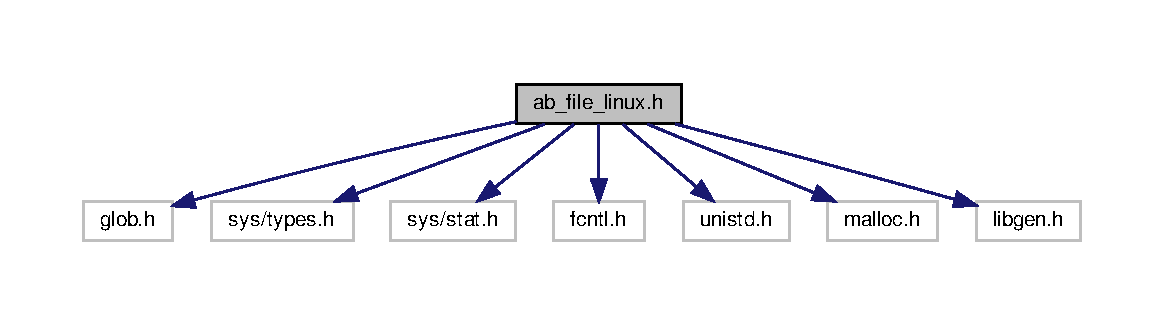
\includegraphics[width=350pt]{d3/d64/ab__file__linux_8h__incl}
\end{center}
\end{figure}
\doxysubsection*{Classes}
\begin{DoxyCompactItemize}
\item 
struct \mbox{\hyperlink{structfile__list}{file\+\_\+list}}
\end{DoxyCompactItemize}

\hypertarget{ab__file__win32_8h}{}\doxysection{ab\+\_\+file\+\_\+win32.\+h File Reference}
\label{ab__file__win32_8h}\index{ab\_file\_win32.h@{ab\_file\_win32.h}}


Windows specific implementation of some file functions.  


{\ttfamily \#include $<$windows.\+h$>$}\newline
{\ttfamily \#include $<$malloc.\+h$>$}\newline
{\ttfamily \#include \char`\"{}ab\+\_\+common.\+h\char`\"{}}\newline
{\ttfamily \#include \char`\"{}ab\+\_\+memory.\+h\char`\"{}}\newline
{\ttfamily \#include \char`\"{}ab\+\_\+string.\+h\char`\"{}}\newline
Include dependency graph for ab\+\_\+file\+\_\+win32.\+h\+:
\nopagebreak
\begin{figure}[H]
\begin{center}
\leavevmode
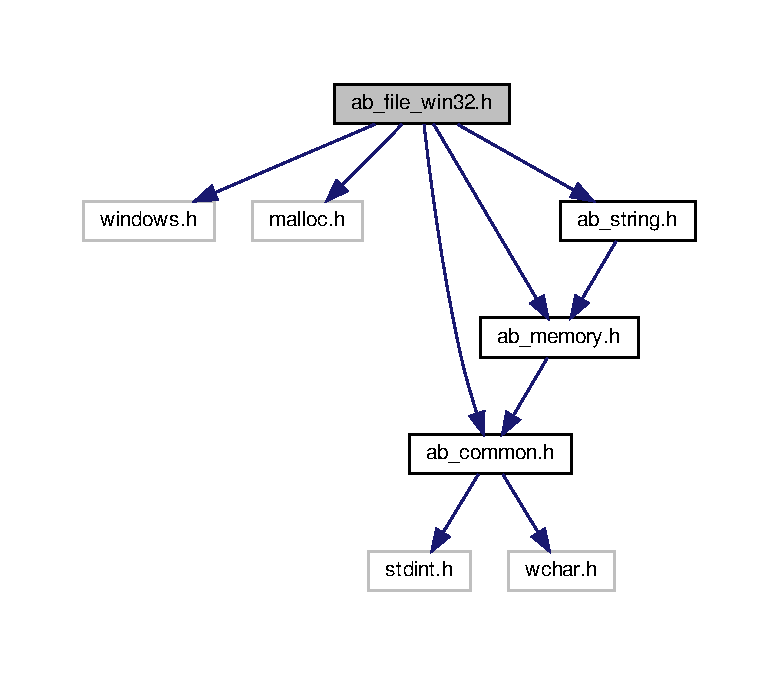
\includegraphics[width=350pt]{d8/d79/ab__file__win32_8h__incl}
\end{center}
\end{figure}
\doxysubsection*{Classes}
\begin{DoxyCompactItemize}
\item 
struct \mbox{\hyperlink{structfile__list}{file\+\_\+list}}
\end{DoxyCompactItemize}
\doxysubsection*{Macros}
\begin{DoxyCompactItemize}
\item 
\#define \mbox{\hyperlink{ab__file__win32_8h_ac7bef5d85e3dcd73eef56ad39ffc84a9}{W\+I\+N32\+\_\+\+L\+E\+A\+N\+\_\+\+A\+N\+D\+\_\+\+M\+E\+AN}}
\end{DoxyCompactItemize}


\doxysubsection{Detailed Description}
Windows specific implementation of some file functions. 

\begin{DoxyAuthor}{Author}
Amos Buchanan 
\end{DoxyAuthor}
\begin{DoxyVersion}{Version}
1.\+0 
\end{DoxyVersion}
\begin{DoxyDate}{Date}
2020 
\end{DoxyDate}
\begin{DoxyCopyright}{Copyright}
\href{https://opensource.org/licenses/MIT}{\texttt{ M\+IT Public License}}
\end{DoxyCopyright}
Windows specific implementation of functions. See \mbox{\hyperlink{ab__file_8h}{ab\+\_\+file.\+h}} for function usage.\hypertarget{ab__file__win32_8h_autotoc_md0}{}\doxysubsection{M\+I\+T License}\label{ab__file__win32_8h_autotoc_md0}
\href{https://opensource.org/licenses/MIT}{\texttt{ M\+IT Public License}}

Copyright 2020 Amos Buchanan

Permission is hereby granted, free of charge, to any person obtaining a copy of this software and associated documentation files (the \char`\"{}\+Software\char`\"{}), to deal in the Software without restriction, including without limitation the rights to use, copy, modify, merge, publish, distribute, sublicense, and/or sell copies of the Software, and to permit persons to whom the Software is furnished to do so, subject to the following conditions\+:

The above copyright notice and this permission notice shall be included in all copies or substantial portions of the Software.

T\+HE S\+O\+F\+T\+W\+A\+RE IS P\+R\+O\+V\+I\+D\+ED \char`\"{}\+A\+S I\+S\char`\"{}, W\+I\+T\+H\+O\+UT W\+A\+R\+R\+A\+N\+TY OF A\+NY K\+I\+ND, E\+X\+P\+R\+E\+SS OR I\+M\+P\+L\+I\+ED, I\+N\+C\+L\+U\+D\+I\+NG B\+UT N\+OT L\+I\+M\+I\+T\+ED TO T\+HE W\+A\+R\+R\+A\+N\+T\+I\+ES OF M\+E\+R\+C\+H\+A\+N\+T\+A\+B\+I\+L\+I\+TY, F\+I\+T\+N\+E\+SS F\+OR A P\+A\+R\+T\+I\+C\+U\+L\+AR P\+U\+R\+P\+O\+SE A\+ND N\+O\+N\+I\+N\+F\+R\+I\+N\+G\+E\+M\+E\+NT. IN NO E\+V\+E\+NT S\+H\+A\+LL T\+HE A\+U\+T\+H\+O\+RS OR C\+O\+P\+Y\+R\+I\+G\+HT H\+O\+L\+D\+E\+RS BE L\+I\+A\+B\+LE F\+OR A\+NY C\+L\+A\+IM, D\+A\+M\+A\+G\+ES OR O\+T\+H\+ER L\+I\+A\+B\+I\+L\+I\+TY, W\+H\+E\+T\+H\+ER IN AN A\+C\+T\+I\+ON OF C\+O\+N\+T\+R\+A\+CT, T\+O\+RT OR O\+T\+H\+E\+R\+W\+I\+SE, A\+R\+I\+S\+I\+NG F\+R\+OM, O\+UT OF OR IN C\+O\+N\+N\+E\+C\+T\+I\+ON W\+I\+TH T\+HE S\+O\+F\+T\+W\+A\+RE OR T\+HE U\+SE OR O\+T\+H\+ER D\+E\+A\+L\+I\+N\+GS IN T\+HE S\+O\+F\+T\+W\+A\+RE. 

\doxysubsection{Macro Definition Documentation}
\mbox{\Hypertarget{ab__file__win32_8h_ac7bef5d85e3dcd73eef56ad39ffc84a9}\label{ab__file__win32_8h_ac7bef5d85e3dcd73eef56ad39ffc84a9}} 
\index{ab\_file\_win32.h@{ab\_file\_win32.h}!WIN32\_LEAN\_AND\_MEAN@{WIN32\_LEAN\_AND\_MEAN}}
\index{WIN32\_LEAN\_AND\_MEAN@{WIN32\_LEAN\_AND\_MEAN}!ab\_file\_win32.h@{ab\_file\_win32.h}}
\doxysubsubsection{\texorpdfstring{WIN32\_LEAN\_AND\_MEAN}{WIN32\_LEAN\_AND\_MEAN}}
{\footnotesize\ttfamily \#define W\+I\+N32\+\_\+\+L\+E\+A\+N\+\_\+\+A\+N\+D\+\_\+\+M\+E\+AN}


\hypertarget{ab__json_8h}{}\section{ab\+\_\+json.\+h File Reference}
\label{ab__json_8h}\index{ab\+\_\+json.\+h@{ab\+\_\+json.\+h}}
{\ttfamily \#include \char`\"{}ab\+\_\+common.\+h\char`\"{}}\newline
{\ttfamily \#include \char`\"{}ab\+\_\+memory.\+h\char`\"{}}\newline
{\ttfamily \#include \char`\"{}ab\+\_\+string.\+h\char`\"{}}\newline
{\ttfamily \#include \char`\"{}jsmn.\+h\char`\"{}}\newline
Include dependency graph for ab\+\_\+json.\+h\+:\nopagebreak
\begin{figure}[H]
\begin{center}
\leavevmode
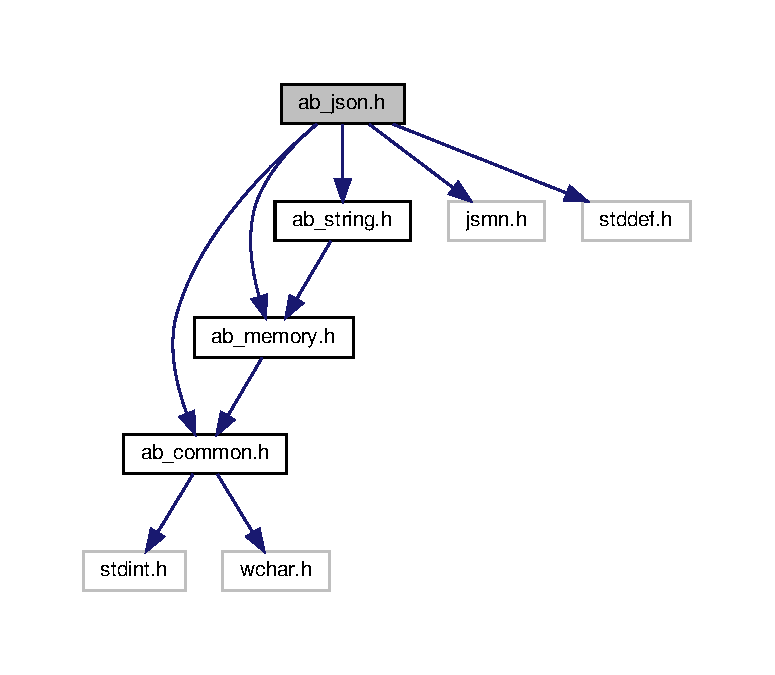
\includegraphics[width=305pt]{d2/d00/ab__json_8h__incl}
\end{center}
\end{figure}
This graph shows which files directly or indirectly include this file\+:\nopagebreak
\begin{figure}[H]
\begin{center}
\leavevmode
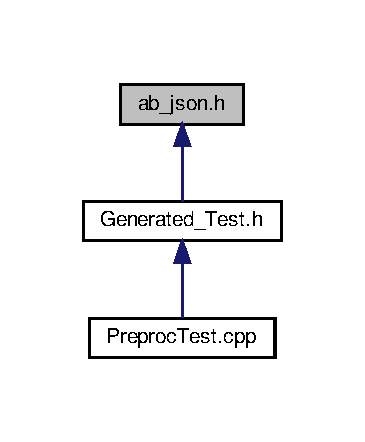
\includegraphics[width=175pt]{d5/d2e/ab__json_8h__dep__incl}
\end{center}
\end{figure}
\subsection*{Macros}
\begin{DoxyCompactItemize}
\item 
\#define \hyperlink{ab__json_8h_aeef9c3539ffb9ed912a2976b67b43d68}{J\+S\+M\+N\+\_\+\+H\+E\+A\+D\+ER}
\end{DoxyCompactItemize}
\subsection*{Enumerations}
\begin{DoxyCompactItemize}
\item 
enum \hyperlink{ab__json_8h_a23451be0e28c552e70c19429684f83cb}{json\+\_\+flags} \{ \hyperlink{ab__json_8h_a23451be0e28c552e70c19429684f83cba12d51163882c2f3f659bf2d2560969b6}{J\+S\+O\+N\+\_\+\+Null} = 0, 
\hyperlink{ab__json_8h_a23451be0e28c552e70c19429684f83cbab892e8229f95855a30a2c10fde71f78e}{J\+S\+O\+N\+\_\+\+Is\+Last\+In\+List} = 1 $<$$<$ 0, 
\hyperlink{ab__json_8h_a23451be0e28c552e70c19429684f83cba4f2bc16d9f2cb38d0e0354342bcd07c1}{J\+S\+O\+N\+\_\+\+Dont\+Use\+Tag} = 1 $<$$<$ 1, 
\hyperlink{ab__json_8h_a23451be0e28c552e70c19429684f83cba508ef51fa6f4677dd0ba7b242f0d269f}{J\+S\+O\+N\+\_\+\+Base\+Object} = 1 $<$$<$ 2
 \}
\end{DoxyCompactItemize}
\subsection*{Functions}
\begin{DoxyCompactItemize}
\item 
\hyperlink{ab__common_8h_ae9b1af5c037e57a98884758875d3a7c4}{s32} \hyperlink{ab__json_8h_a2b3b6ac206a0ad8367ef1b795ae06d94}{Parse\+Json} (\hyperlink{structmemory__arena}{memory\+\_\+arena} $\ast$Volatile\+Memory, char const $\ast$Json, size\+\_\+t Json\+Length, \hyperlink{structjsmntok__t}{jsmntok\+\_\+t} $\ast$$\ast$Token\+Array)
\item 
\hyperlink{ab__common_8h_afaa62991928fb9fb18ff0db62a040aba}{u32} \hyperlink{ab__json_8h_a2c85de19a5702595393c516b1637896b}{Start\+Group} (char $\ast$, \hyperlink{ab__common_8h_afaa62991928fb9fb18ff0db62a040aba}{u32} Max\+Length)
\item 
\hyperlink{ab__common_8h_afaa62991928fb9fb18ff0db62a040aba}{u32} \hyperlink{ab__json_8h_a8d4a5895fda267713cbb9818d27e1a57}{End\+Group} (char $\ast$, \hyperlink{ab__common_8h_afaa62991928fb9fb18ff0db62a040aba}{u32} Max\+Length, \hyperlink{ab__common_8h_a70e369648385b50f2d0588e8e8745275}{b8} is\+Last)
\item 
\hyperlink{structabs__stringptr}{abs\+\_\+stringptr} \hyperlink{ab__json_8h_a6d809a2544db46f751036c308b9ec380}{Token\+To\+String\+Ptr} (char const $\ast$Json, \hyperlink{structjsmntok__t}{jsmntok\+\_\+t} $\ast$Token)
\item 
\hyperlink{ab__common_8h_a70e369648385b50f2d0588e8e8745275}{b8} \hyperlink{ab__json_8h_adc0dbd5f4b093577ebd0b4e252e17731}{Token\+Equals} (char const $\ast$Json, \hyperlink{structjsmntok__t}{jsmntok\+\_\+t} $\ast$Token, char const $\ast$Value)
\end{DoxyCompactItemize}


\subsection{Macro Definition Documentation}
\mbox{\Hypertarget{ab__json_8h_aeef9c3539ffb9ed912a2976b67b43d68}\label{ab__json_8h_aeef9c3539ffb9ed912a2976b67b43d68}} 
\index{ab\+\_\+json.\+h@{ab\+\_\+json.\+h}!J\+S\+M\+N\+\_\+\+H\+E\+A\+D\+ER@{J\+S\+M\+N\+\_\+\+H\+E\+A\+D\+ER}}
\index{J\+S\+M\+N\+\_\+\+H\+E\+A\+D\+ER@{J\+S\+M\+N\+\_\+\+H\+E\+A\+D\+ER}!ab\+\_\+json.\+h@{ab\+\_\+json.\+h}}
\subsubsection{\texorpdfstring{J\+S\+M\+N\+\_\+\+H\+E\+A\+D\+ER}{JSMN\_HEADER}}
{\footnotesize\ttfamily \#define J\+S\+M\+N\+\_\+\+H\+E\+A\+D\+ER}



\subsection{Enumeration Type Documentation}
\mbox{\Hypertarget{ab__json_8h_a23451be0e28c552e70c19429684f83cb}\label{ab__json_8h_a23451be0e28c552e70c19429684f83cb}} 
\index{ab\+\_\+json.\+h@{ab\+\_\+json.\+h}!json\+\_\+flags@{json\+\_\+flags}}
\index{json\+\_\+flags@{json\+\_\+flags}!ab\+\_\+json.\+h@{ab\+\_\+json.\+h}}
\subsubsection{\texorpdfstring{json\+\_\+flags}{json\_flags}}
{\footnotesize\ttfamily enum \hyperlink{ab__json_8h_a23451be0e28c552e70c19429684f83cb}{json\+\_\+flags}}

\begin{DoxyEnumFields}{Enumerator}
\raisebox{\heightof{T}}[0pt][0pt]{\index{J\+S\+O\+N\+\_\+\+Null@{J\+S\+O\+N\+\_\+\+Null}!ab\+\_\+json.\+h@{ab\+\_\+json.\+h}}\index{ab\+\_\+json.\+h@{ab\+\_\+json.\+h}!J\+S\+O\+N\+\_\+\+Null@{J\+S\+O\+N\+\_\+\+Null}}}\mbox{\Hypertarget{ab__json_8h_a23451be0e28c552e70c19429684f83cba12d51163882c2f3f659bf2d2560969b6}\label{ab__json_8h_a23451be0e28c552e70c19429684f83cba12d51163882c2f3f659bf2d2560969b6}} 
J\+S\+O\+N\+\_\+\+Null&\\
\hline

\raisebox{\heightof{T}}[0pt][0pt]{\index{J\+S\+O\+N\+\_\+\+Is\+Last\+In\+List@{J\+S\+O\+N\+\_\+\+Is\+Last\+In\+List}!ab\+\_\+json.\+h@{ab\+\_\+json.\+h}}\index{ab\+\_\+json.\+h@{ab\+\_\+json.\+h}!J\+S\+O\+N\+\_\+\+Is\+Last\+In\+List@{J\+S\+O\+N\+\_\+\+Is\+Last\+In\+List}}}\mbox{\Hypertarget{ab__json_8h_a23451be0e28c552e70c19429684f83cbab892e8229f95855a30a2c10fde71f78e}\label{ab__json_8h_a23451be0e28c552e70c19429684f83cbab892e8229f95855a30a2c10fde71f78e}} 
J\+S\+O\+N\+\_\+\+Is\+Last\+In\+List&\\
\hline

\raisebox{\heightof{T}}[0pt][0pt]{\index{J\+S\+O\+N\+\_\+\+Dont\+Use\+Tag@{J\+S\+O\+N\+\_\+\+Dont\+Use\+Tag}!ab\+\_\+json.\+h@{ab\+\_\+json.\+h}}\index{ab\+\_\+json.\+h@{ab\+\_\+json.\+h}!J\+S\+O\+N\+\_\+\+Dont\+Use\+Tag@{J\+S\+O\+N\+\_\+\+Dont\+Use\+Tag}}}\mbox{\Hypertarget{ab__json_8h_a23451be0e28c552e70c19429684f83cba4f2bc16d9f2cb38d0e0354342bcd07c1}\label{ab__json_8h_a23451be0e28c552e70c19429684f83cba4f2bc16d9f2cb38d0e0354342bcd07c1}} 
J\+S\+O\+N\+\_\+\+Dont\+Use\+Tag&\\
\hline

\raisebox{\heightof{T}}[0pt][0pt]{\index{J\+S\+O\+N\+\_\+\+Base\+Object@{J\+S\+O\+N\+\_\+\+Base\+Object}!ab\+\_\+json.\+h@{ab\+\_\+json.\+h}}\index{ab\+\_\+json.\+h@{ab\+\_\+json.\+h}!J\+S\+O\+N\+\_\+\+Base\+Object@{J\+S\+O\+N\+\_\+\+Base\+Object}}}\mbox{\Hypertarget{ab__json_8h_a23451be0e28c552e70c19429684f83cba508ef51fa6f4677dd0ba7b242f0d269f}\label{ab__json_8h_a23451be0e28c552e70c19429684f83cba508ef51fa6f4677dd0ba7b242f0d269f}} 
J\+S\+O\+N\+\_\+\+Base\+Object&\\
\hline

\end{DoxyEnumFields}


\subsection{Function Documentation}
\mbox{\Hypertarget{ab__json_8h_a8d4a5895fda267713cbb9818d27e1a57}\label{ab__json_8h_a8d4a5895fda267713cbb9818d27e1a57}} 
\index{ab\+\_\+json.\+h@{ab\+\_\+json.\+h}!End\+Group@{End\+Group}}
\index{End\+Group@{End\+Group}!ab\+\_\+json.\+h@{ab\+\_\+json.\+h}}
\subsubsection{\texorpdfstring{End\+Group()}{EndGroup()}}
{\footnotesize\ttfamily \hyperlink{ab__common_8h_afaa62991928fb9fb18ff0db62a040aba}{u32} End\+Group (\begin{DoxyParamCaption}\item[{char $\ast$}]{,  }\item[{\hyperlink{ab__common_8h_afaa62991928fb9fb18ff0db62a040aba}{u32}}]{Max\+Length,  }\item[{\hyperlink{ab__common_8h_a70e369648385b50f2d0588e8e8745275}{b8}}]{is\+Last }\end{DoxyParamCaption})\hspace{0.3cm}{\ttfamily [inline]}}

\mbox{\Hypertarget{ab__json_8h_a2b3b6ac206a0ad8367ef1b795ae06d94}\label{ab__json_8h_a2b3b6ac206a0ad8367ef1b795ae06d94}} 
\index{ab\+\_\+json.\+h@{ab\+\_\+json.\+h}!Parse\+Json@{Parse\+Json}}
\index{Parse\+Json@{Parse\+Json}!ab\+\_\+json.\+h@{ab\+\_\+json.\+h}}
\subsubsection{\texorpdfstring{Parse\+Json()}{ParseJson()}}
{\footnotesize\ttfamily \hyperlink{ab__common_8h_ae9b1af5c037e57a98884758875d3a7c4}{s32} Parse\+Json (\begin{DoxyParamCaption}\item[{\hyperlink{structmemory__arena}{memory\+\_\+arena} $\ast$}]{Volatile\+Memory,  }\item[{char const $\ast$}]{Json,  }\item[{size\+\_\+t}]{Json\+Length,  }\item[{\hyperlink{structjsmntok__t}{jsmntok\+\_\+t} $\ast$$\ast$}]{Token\+Array }\end{DoxyParamCaption})\hspace{0.3cm}{\ttfamily [inline]}}

\mbox{\Hypertarget{ab__json_8h_a2c85de19a5702595393c516b1637896b}\label{ab__json_8h_a2c85de19a5702595393c516b1637896b}} 
\index{ab\+\_\+json.\+h@{ab\+\_\+json.\+h}!Start\+Group@{Start\+Group}}
\index{Start\+Group@{Start\+Group}!ab\+\_\+json.\+h@{ab\+\_\+json.\+h}}
\subsubsection{\texorpdfstring{Start\+Group()}{StartGroup()}}
{\footnotesize\ttfamily \hyperlink{ab__common_8h_afaa62991928fb9fb18ff0db62a040aba}{u32} Start\+Group (\begin{DoxyParamCaption}\item[{char $\ast$}]{,  }\item[{\hyperlink{ab__common_8h_afaa62991928fb9fb18ff0db62a040aba}{u32}}]{Max\+Length }\end{DoxyParamCaption})\hspace{0.3cm}{\ttfamily [inline]}}

\mbox{\Hypertarget{ab__json_8h_adc0dbd5f4b093577ebd0b4e252e17731}\label{ab__json_8h_adc0dbd5f4b093577ebd0b4e252e17731}} 
\index{ab\+\_\+json.\+h@{ab\+\_\+json.\+h}!Token\+Equals@{Token\+Equals}}
\index{Token\+Equals@{Token\+Equals}!ab\+\_\+json.\+h@{ab\+\_\+json.\+h}}
\subsubsection{\texorpdfstring{Token\+Equals()}{TokenEquals()}}
{\footnotesize\ttfamily \hyperlink{ab__common_8h_a70e369648385b50f2d0588e8e8745275}{b8} Token\+Equals (\begin{DoxyParamCaption}\item[{char const $\ast$}]{Json,  }\item[{\hyperlink{structjsmntok__t}{jsmntok\+\_\+t} $\ast$}]{Token,  }\item[{char const $\ast$}]{Value }\end{DoxyParamCaption})\hspace{0.3cm}{\ttfamily [inline]}}

\mbox{\Hypertarget{ab__json_8h_a6d809a2544db46f751036c308b9ec380}\label{ab__json_8h_a6d809a2544db46f751036c308b9ec380}} 
\index{ab\+\_\+json.\+h@{ab\+\_\+json.\+h}!Token\+To\+String\+Ptr@{Token\+To\+String\+Ptr}}
\index{Token\+To\+String\+Ptr@{Token\+To\+String\+Ptr}!ab\+\_\+json.\+h@{ab\+\_\+json.\+h}}
\subsubsection{\texorpdfstring{Token\+To\+String\+Ptr()}{TokenToStringPtr()}}
{\footnotesize\ttfamily \hyperlink{structabs__stringptr}{abs\+\_\+stringptr} Token\+To\+String\+Ptr (\begin{DoxyParamCaption}\item[{char const $\ast$}]{Json,  }\item[{\hyperlink{structjsmntok__t}{jsmntok\+\_\+t} $\ast$}]{Token }\end{DoxyParamCaption})\hspace{0.3cm}{\ttfamily [inline]}}


\hypertarget{ab__logger_8h}{}\doxysection{ab\+\_\+logger.\+h File Reference}
\label{ab__logger_8h}\index{ab\_logger.h@{ab\_logger.h}}
{\ttfamily \#include \char`\"{}czmq.\+h\char`\"{}}\newline
{\ttfamily \#include \char`\"{}ab\+\_\+common.\+h\char`\"{}}\newline
Include dependency graph for ab\+\_\+logger.\+h\+:\nopagebreak
\begin{figure}[H]
\begin{center}
\leavevmode
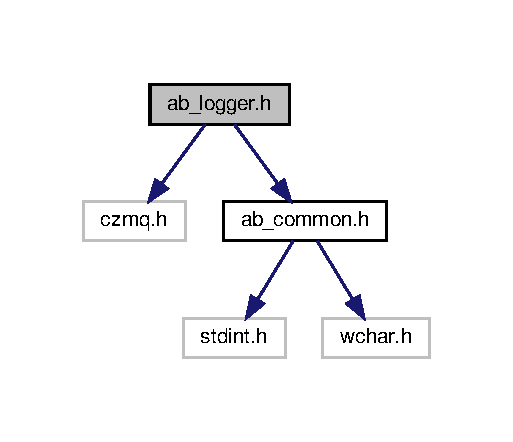
\includegraphics[width=246pt]{d3/d74/ab__logger_8h__incl}
\end{center}
\end{figure}
\doxysubsection*{Macros}
\begin{DoxyCompactItemize}
\item 
\#define \mbox{\hyperlink{ab__logger_8h_a1c3af1ceb74203276ce7ca7ec60b6e63}{abl\+\_\+trace}}(Logger,  Fmt, ...)~\mbox{\hyperlink{ab__logger_8h_a7d0be7575c2768d56ad5bdc391d3d769}{abl\+\_\+log}}(Logger, L\+O\+G\+\_\+\+T\+R\+A\+CE, \+\_\+\+\_\+\+F\+I\+L\+E\+\_\+\+\_\+, \+\_\+\+\_\+\+L\+I\+N\+E\+\_\+\+\_\+, Fmt, \+\_\+\+\_\+\+V\+A\+\_\+\+A\+R\+G\+S\+\_\+\+\_\+)
\item 
\#define \mbox{\hyperlink{ab__logger_8h_af0d95724956482b6abce967bec5bca6d}{abl\+\_\+debug}}(Logger,  Fmt, ...)~\mbox{\hyperlink{ab__logger_8h_a7d0be7575c2768d56ad5bdc391d3d769}{abl\+\_\+log}}(Logger, L\+O\+G\+\_\+\+D\+E\+B\+UG, \+\_\+\+\_\+\+F\+I\+L\+E\+\_\+\+\_\+, \+\_\+\+\_\+\+L\+I\+N\+E\+\_\+\+\_\+, Fmt, \+\_\+\+\_\+\+V\+A\+\_\+\+A\+R\+G\+S\+\_\+\+\_\+)
\item 
\#define \mbox{\hyperlink{ab__logger_8h_a0e01c4cfce56ca553e16e2f85bb9f0fe}{abl\+\_\+info}}(Logger,  Fmt, ...)~\mbox{\hyperlink{ab__logger_8h_a7d0be7575c2768d56ad5bdc391d3d769}{abl\+\_\+log}}(Logger, L\+O\+G\+\_\+\+I\+N\+FO,  \+\_\+\+\_\+\+F\+I\+L\+E\+\_\+\+\_\+, \+\_\+\+\_\+\+L\+I\+N\+E\+\_\+\+\_\+, Fmt, \+\_\+\+\_\+\+V\+A\+\_\+\+A\+R\+G\+S\+\_\+\+\_\+)
\item 
\#define \mbox{\hyperlink{ab__logger_8h_ace87fcfe98d7bb16ff20b09002b0f41b}{abl\+\_\+warn}}(Logger,  Fmt, ...)~\mbox{\hyperlink{ab__logger_8h_a7d0be7575c2768d56ad5bdc391d3d769}{abl\+\_\+log}}(Logger, L\+O\+G\+\_\+\+W\+A\+RN,  \+\_\+\+\_\+\+F\+I\+L\+E\+\_\+\+\_\+, \+\_\+\+\_\+\+L\+I\+N\+E\+\_\+\+\_\+, Fmt, \+\_\+\+\_\+\+V\+A\+\_\+\+A\+R\+G\+S\+\_\+\+\_\+)
\item 
\#define \mbox{\hyperlink{ab__logger_8h_a9701d37f9ea32885eb4435456b54380c}{abl\+\_\+error}}(Logger,  Fmt, ...)~\mbox{\hyperlink{ab__logger_8h_a7d0be7575c2768d56ad5bdc391d3d769}{abl\+\_\+log}}(Logger, L\+O\+G\+\_\+\+E\+R\+R\+OR, \+\_\+\+\_\+\+F\+I\+L\+E\+\_\+\+\_\+, \+\_\+\+\_\+\+L\+I\+N\+E\+\_\+\+\_\+, Fmt, \+\_\+\+\_\+\+V\+A\+\_\+\+A\+R\+G\+S\+\_\+\+\_\+)
\item 
\#define \mbox{\hyperlink{ab__logger_8h_a56cde45c39126f008262c3d94e03e9b8}{abl\+\_\+fatal}}(Logger,  Fmt, ...)~\mbox{\hyperlink{ab__logger_8h_a7d0be7575c2768d56ad5bdc391d3d769}{abl\+\_\+log}}(Logger, L\+O\+G\+\_\+\+F\+A\+T\+AL, \+\_\+\+\_\+\+F\+I\+L\+E\+\_\+\+\_\+, \+\_\+\+\_\+\+L\+I\+N\+E\+\_\+\+\_\+, Fmt, \+\_\+\+\_\+\+V\+A\+\_\+\+A\+R\+G\+S\+\_\+\+\_\+)
\end{DoxyCompactItemize}
\doxysubsection*{Enumerations}
\begin{DoxyCompactItemize}
\item 
enum \mbox{\hyperlink{ab__logger_8h_ad09c15c023f4bd204786f7c031c45787}{abl\+\_\+log\+\_\+level}} \{ \newline
\mbox{\hyperlink{ab__logger_8h_ad09c15c023f4bd204786f7c031c45787a7fccde42da961232bd100be86f2c32b1}{A\+B\+L\+\_\+\+T\+R\+A\+CE}}, 
\mbox{\hyperlink{ab__logger_8h_ad09c15c023f4bd204786f7c031c45787a4a4d2ab22d6f6be96611dfc75021117e}{A\+B\+L\+\_\+\+D\+E\+B\+UG}}, 
\mbox{\hyperlink{ab__logger_8h_ad09c15c023f4bd204786f7c031c45787a72e995c24ee1e50bfa27759c4c2c0bee}{A\+B\+L\+\_\+\+I\+N\+FO}}, 
\mbox{\hyperlink{ab__logger_8h_ad09c15c023f4bd204786f7c031c45787af4a847c0c5d6fe01ec92ab29b2d21144}{A\+B\+L\+\_\+\+W\+A\+RN}}, 
\newline
\mbox{\hyperlink{ab__logger_8h_ad09c15c023f4bd204786f7c031c45787a11c5fd338567ea5a3cdff6dfec3b7b5f}{A\+B\+L\+\_\+\+E\+R\+R\+OR}}, 
\mbox{\hyperlink{ab__logger_8h_ad09c15c023f4bd204786f7c031c45787a3c083097aaf5d4784c9513b0eba01e75}{A\+B\+L\+\_\+\+F\+A\+T\+AL}}
 \}
\end{DoxyCompactItemize}
\doxysubsection*{Functions}
\begin{DoxyCompactItemize}
\item 
void \mbox{\hyperlink{ab__logger_8h_adc94b6d140adcd78c7f0bb2fce524667}{abl\+\_\+start\+\_\+server}} (ab\+\_\+log $\ast$Logger, \mbox{\hyperlink{ab__common_8h_ae9b1af5c037e57a98884758875d3a7c4}{s32}} Port)
\item 
void \mbox{\hyperlink{ab__logger_8h_adce1f3ea2b2bd6eea7e33b63fd8c0499}{abl\+\_\+set\+\_\+fp}} (ab\+\_\+log $\ast$Logger, F\+I\+LE $\ast$fp)
\item 
void \mbox{\hyperlink{ab__logger_8h_ad9700e7478bc6850a033e6c1cc6eeaa1}{abl\+\_\+set\+\_\+level}} (ab\+\_\+log $\ast$Logger, \mbox{\hyperlink{ab__logger_8h_ad09c15c023f4bd204786f7c031c45787}{abl\+\_\+log\+\_\+level}} Level)
\item 
void \mbox{\hyperlink{ab__logger_8h_af26d8d70a5083e1d9c994c3e3f0b5622}{abl\+\_\+set\+\_\+quiet}} (ab\+\_\+log $\ast$Logger, \mbox{\hyperlink{ab__common_8h_a70e369648385b50f2d0588e8e8745275}{b8}} is\+Quiet)
\item 
void \mbox{\hyperlink{ab__logger_8h_a830f7af6399163b2ac8c6443042f97c7}{abl\+\_\+stop\+\_\+server}} (ab\+\_\+log $\ast$Logger)
\item 
void \mbox{\hyperlink{ab__logger_8h_a7d0be7575c2768d56ad5bdc391d3d769}{abl\+\_\+log}} (ab\+\_\+log $\ast$Logger, \mbox{\hyperlink{ab__logger_8h_ad09c15c023f4bd204786f7c031c45787}{abl\+\_\+log\+\_\+level}} Level, const char $\ast$File, \mbox{\hyperlink{ab__common_8h_ae9b1af5c037e57a98884758875d3a7c4}{s32}} Line, const char $\ast$Fmt,...)
\end{DoxyCompactItemize}


\doxysubsection{Macro Definition Documentation}
\mbox{\Hypertarget{ab__logger_8h_af0d95724956482b6abce967bec5bca6d}\label{ab__logger_8h_af0d95724956482b6abce967bec5bca6d}} 
\index{ab\_logger.h@{ab\_logger.h}!abl\_debug@{abl\_debug}}
\index{abl\_debug@{abl\_debug}!ab\_logger.h@{ab\_logger.h}}
\doxysubsubsection{\texorpdfstring{abl\_debug}{abl\_debug}}
{\footnotesize\ttfamily \#define abl\+\_\+debug(\begin{DoxyParamCaption}\item[{}]{Logger,  }\item[{}]{Fmt,  }\item[{}]{... }\end{DoxyParamCaption})~\mbox{\hyperlink{ab__logger_8h_a7d0be7575c2768d56ad5bdc391d3d769}{abl\+\_\+log}}(Logger, L\+O\+G\+\_\+\+D\+E\+B\+UG, \+\_\+\+\_\+\+F\+I\+L\+E\+\_\+\+\_\+, \+\_\+\+\_\+\+L\+I\+N\+E\+\_\+\+\_\+, Fmt, \+\_\+\+\_\+\+V\+A\+\_\+\+A\+R\+G\+S\+\_\+\+\_\+)}

\mbox{\Hypertarget{ab__logger_8h_a9701d37f9ea32885eb4435456b54380c}\label{ab__logger_8h_a9701d37f9ea32885eb4435456b54380c}} 
\index{ab\_logger.h@{ab\_logger.h}!abl\_error@{abl\_error}}
\index{abl\_error@{abl\_error}!ab\_logger.h@{ab\_logger.h}}
\doxysubsubsection{\texorpdfstring{abl\_error}{abl\_error}}
{\footnotesize\ttfamily \#define abl\+\_\+error(\begin{DoxyParamCaption}\item[{}]{Logger,  }\item[{}]{Fmt,  }\item[{}]{... }\end{DoxyParamCaption})~\mbox{\hyperlink{ab__logger_8h_a7d0be7575c2768d56ad5bdc391d3d769}{abl\+\_\+log}}(Logger, L\+O\+G\+\_\+\+E\+R\+R\+OR, \+\_\+\+\_\+\+F\+I\+L\+E\+\_\+\+\_\+, \+\_\+\+\_\+\+L\+I\+N\+E\+\_\+\+\_\+, Fmt, \+\_\+\+\_\+\+V\+A\+\_\+\+A\+R\+G\+S\+\_\+\+\_\+)}

\mbox{\Hypertarget{ab__logger_8h_a56cde45c39126f008262c3d94e03e9b8}\label{ab__logger_8h_a56cde45c39126f008262c3d94e03e9b8}} 
\index{ab\_logger.h@{ab\_logger.h}!abl\_fatal@{abl\_fatal}}
\index{abl\_fatal@{abl\_fatal}!ab\_logger.h@{ab\_logger.h}}
\doxysubsubsection{\texorpdfstring{abl\_fatal}{abl\_fatal}}
{\footnotesize\ttfamily \#define abl\+\_\+fatal(\begin{DoxyParamCaption}\item[{}]{Logger,  }\item[{}]{Fmt,  }\item[{}]{... }\end{DoxyParamCaption})~\mbox{\hyperlink{ab__logger_8h_a7d0be7575c2768d56ad5bdc391d3d769}{abl\+\_\+log}}(Logger, L\+O\+G\+\_\+\+F\+A\+T\+AL, \+\_\+\+\_\+\+F\+I\+L\+E\+\_\+\+\_\+, \+\_\+\+\_\+\+L\+I\+N\+E\+\_\+\+\_\+, Fmt, \+\_\+\+\_\+\+V\+A\+\_\+\+A\+R\+G\+S\+\_\+\+\_\+)}

\mbox{\Hypertarget{ab__logger_8h_a0e01c4cfce56ca553e16e2f85bb9f0fe}\label{ab__logger_8h_a0e01c4cfce56ca553e16e2f85bb9f0fe}} 
\index{ab\_logger.h@{ab\_logger.h}!abl\_info@{abl\_info}}
\index{abl\_info@{abl\_info}!ab\_logger.h@{ab\_logger.h}}
\doxysubsubsection{\texorpdfstring{abl\_info}{abl\_info}}
{\footnotesize\ttfamily \#define abl\+\_\+info(\begin{DoxyParamCaption}\item[{}]{Logger,  }\item[{}]{Fmt,  }\item[{}]{... }\end{DoxyParamCaption})~\mbox{\hyperlink{ab__logger_8h_a7d0be7575c2768d56ad5bdc391d3d769}{abl\+\_\+log}}(Logger, L\+O\+G\+\_\+\+I\+N\+FO,  \+\_\+\+\_\+\+F\+I\+L\+E\+\_\+\+\_\+, \+\_\+\+\_\+\+L\+I\+N\+E\+\_\+\+\_\+, Fmt, \+\_\+\+\_\+\+V\+A\+\_\+\+A\+R\+G\+S\+\_\+\+\_\+)}

\mbox{\Hypertarget{ab__logger_8h_a1c3af1ceb74203276ce7ca7ec60b6e63}\label{ab__logger_8h_a1c3af1ceb74203276ce7ca7ec60b6e63}} 
\index{ab\_logger.h@{ab\_logger.h}!abl\_trace@{abl\_trace}}
\index{abl\_trace@{abl\_trace}!ab\_logger.h@{ab\_logger.h}}
\doxysubsubsection{\texorpdfstring{abl\_trace}{abl\_trace}}
{\footnotesize\ttfamily \#define abl\+\_\+trace(\begin{DoxyParamCaption}\item[{}]{Logger,  }\item[{}]{Fmt,  }\item[{}]{... }\end{DoxyParamCaption})~\mbox{\hyperlink{ab__logger_8h_a7d0be7575c2768d56ad5bdc391d3d769}{abl\+\_\+log}}(Logger, L\+O\+G\+\_\+\+T\+R\+A\+CE, \+\_\+\+\_\+\+F\+I\+L\+E\+\_\+\+\_\+, \+\_\+\+\_\+\+L\+I\+N\+E\+\_\+\+\_\+, Fmt, \+\_\+\+\_\+\+V\+A\+\_\+\+A\+R\+G\+S\+\_\+\+\_\+)}

If multi-\/threaded, must declare a logger for use. \mbox{\Hypertarget{ab__logger_8h_ace87fcfe98d7bb16ff20b09002b0f41b}\label{ab__logger_8h_ace87fcfe98d7bb16ff20b09002b0f41b}} 
\index{ab\_logger.h@{ab\_logger.h}!abl\_warn@{abl\_warn}}
\index{abl\_warn@{abl\_warn}!ab\_logger.h@{ab\_logger.h}}
\doxysubsubsection{\texorpdfstring{abl\_warn}{abl\_warn}}
{\footnotesize\ttfamily \#define abl\+\_\+warn(\begin{DoxyParamCaption}\item[{}]{Logger,  }\item[{}]{Fmt,  }\item[{}]{... }\end{DoxyParamCaption})~\mbox{\hyperlink{ab__logger_8h_a7d0be7575c2768d56ad5bdc391d3d769}{abl\+\_\+log}}(Logger, L\+O\+G\+\_\+\+W\+A\+RN,  \+\_\+\+\_\+\+F\+I\+L\+E\+\_\+\+\_\+, \+\_\+\+\_\+\+L\+I\+N\+E\+\_\+\+\_\+, Fmt, \+\_\+\+\_\+\+V\+A\+\_\+\+A\+R\+G\+S\+\_\+\+\_\+)}



\doxysubsection{Enumeration Type Documentation}
\mbox{\Hypertarget{ab__logger_8h_ad09c15c023f4bd204786f7c031c45787}\label{ab__logger_8h_ad09c15c023f4bd204786f7c031c45787}} 
\index{ab\_logger.h@{ab\_logger.h}!abl\_log\_level@{abl\_log\_level}}
\index{abl\_log\_level@{abl\_log\_level}!ab\_logger.h@{ab\_logger.h}}
\doxysubsubsection{\texorpdfstring{abl\_log\_level}{abl\_log\_level}}
{\footnotesize\ttfamily enum \mbox{\hyperlink{ab__logger_8h_ad09c15c023f4bd204786f7c031c45787}{abl\+\_\+log\+\_\+level}}}

Logger. Version\+: 1.\+0 Network logger using czmq. Will log to S\+T\+D\+E\+RR, a file and/or to a czmq network, depending on setup. S\+T\+D\+E\+RR logging not garunteed to be threadsafe, don\textquotesingle{}t do it. Logging multiple threads to the same file not garunteed to be threadsafe. C\+Z\+MQ logging is threadsafe subject to the restrictions of C\+Z\+MQ.

Basically, use a different ab\+\_\+log for each thread and you should be ok.

This is a single-\/file-\/library. You may include the file anywhere in your source. Only once in your code, define the following\+:


\begin{DoxyCode}{0}
\DoxyCodeLine{\textcolor{preprocessor}{\#define AB\_LOGGER\_SRC}}
\DoxyCodeLine{\textcolor{preprocessor}{\#include "{}ab\_logger.h"{}}}
\end{DoxyCode}


This will include the source.

There\textquotesingle{}s a single-\/thread use that uses a global logger. Define the following\+: 
\begin{DoxyCode}{0}
\DoxyCodeLine{\textcolor{preprocessor}{\#define AB\_LOGGER\_SINGLETHREAD}}
\end{DoxyCode}


To use color on S\+T\+D\+E\+RR\+: 
\begin{DoxyCode}{0}
\DoxyCodeLine{\textcolor{preprocessor}{\#define AB\_LOGGER\_USE\_COLOR}}
\end{DoxyCode}


Available levels\+: A\+B\+L\+\_\+\+T\+R\+A\+CE, A\+B\+L\+\_\+\+D\+E\+B\+UG, A\+B\+L\+\_\+\+I\+N\+FO, A\+B\+L\+\_\+\+W\+A\+RN, A\+B\+L\+\_\+\+E\+R\+R\+OR, A\+B\+L\+\_\+\+F\+A\+T\+AL

example usage\+: abl\+\_\+log Logger = \{\}; abl\+\_\+set\+\_\+level(\&\+Logger, A\+B\+L\+\_\+\+I\+N\+F\+O); abl\+\_\+start\+\_\+server(\&\+Logger, 555); abl\+\_\+info(\&Logger, \char`\"{}\+Some log\char`\"{}); abl\+\_\+info(\&Logger, \char`\"{}\+More Info, \%d\char`\"{}, errno); abl\+\_\+stop\+\_\+server(\&\+Logger); \begin{DoxyEnumFields}{Enumerator}
\raisebox{\heightof{T}}[0pt][0pt]{\index{ABL\_TRACE@{ABL\_TRACE}!ab\_logger.h@{ab\_logger.h}}\index{ab\_logger.h@{ab\_logger.h}!ABL\_TRACE@{ABL\_TRACE}}}\mbox{\Hypertarget{ab__logger_8h_ad09c15c023f4bd204786f7c031c45787a7fccde42da961232bd100be86f2c32b1}\label{ab__logger_8h_ad09c15c023f4bd204786f7c031c45787a7fccde42da961232bd100be86f2c32b1}} 
A\+B\+L\+\_\+\+T\+R\+A\+CE&\\
\hline

\raisebox{\heightof{T}}[0pt][0pt]{\index{ABL\_DEBUG@{ABL\_DEBUG}!ab\_logger.h@{ab\_logger.h}}\index{ab\_logger.h@{ab\_logger.h}!ABL\_DEBUG@{ABL\_DEBUG}}}\mbox{\Hypertarget{ab__logger_8h_ad09c15c023f4bd204786f7c031c45787a4a4d2ab22d6f6be96611dfc75021117e}\label{ab__logger_8h_ad09c15c023f4bd204786f7c031c45787a4a4d2ab22d6f6be96611dfc75021117e}} 
A\+B\+L\+\_\+\+D\+E\+B\+UG&\\
\hline

\raisebox{\heightof{T}}[0pt][0pt]{\index{ABL\_INFO@{ABL\_INFO}!ab\_logger.h@{ab\_logger.h}}\index{ab\_logger.h@{ab\_logger.h}!ABL\_INFO@{ABL\_INFO}}}\mbox{\Hypertarget{ab__logger_8h_ad09c15c023f4bd204786f7c031c45787a72e995c24ee1e50bfa27759c4c2c0bee}\label{ab__logger_8h_ad09c15c023f4bd204786f7c031c45787a72e995c24ee1e50bfa27759c4c2c0bee}} 
A\+B\+L\+\_\+\+I\+N\+FO&\\
\hline

\raisebox{\heightof{T}}[0pt][0pt]{\index{ABL\_WARN@{ABL\_WARN}!ab\_logger.h@{ab\_logger.h}}\index{ab\_logger.h@{ab\_logger.h}!ABL\_WARN@{ABL\_WARN}}}\mbox{\Hypertarget{ab__logger_8h_ad09c15c023f4bd204786f7c031c45787af4a847c0c5d6fe01ec92ab29b2d21144}\label{ab__logger_8h_ad09c15c023f4bd204786f7c031c45787af4a847c0c5d6fe01ec92ab29b2d21144}} 
A\+B\+L\+\_\+\+W\+A\+RN&\\
\hline

\raisebox{\heightof{T}}[0pt][0pt]{\index{ABL\_ERROR@{ABL\_ERROR}!ab\_logger.h@{ab\_logger.h}}\index{ab\_logger.h@{ab\_logger.h}!ABL\_ERROR@{ABL\_ERROR}}}\mbox{\Hypertarget{ab__logger_8h_ad09c15c023f4bd204786f7c031c45787a11c5fd338567ea5a3cdff6dfec3b7b5f}\label{ab__logger_8h_ad09c15c023f4bd204786f7c031c45787a11c5fd338567ea5a3cdff6dfec3b7b5f}} 
A\+B\+L\+\_\+\+E\+R\+R\+OR&\\
\hline

\raisebox{\heightof{T}}[0pt][0pt]{\index{ABL\_FATAL@{ABL\_FATAL}!ab\_logger.h@{ab\_logger.h}}\index{ab\_logger.h@{ab\_logger.h}!ABL\_FATAL@{ABL\_FATAL}}}\mbox{\Hypertarget{ab__logger_8h_ad09c15c023f4bd204786f7c031c45787a3c083097aaf5d4784c9513b0eba01e75}\label{ab__logger_8h_ad09c15c023f4bd204786f7c031c45787a3c083097aaf5d4784c9513b0eba01e75}} 
A\+B\+L\+\_\+\+F\+A\+T\+AL&\\
\hline

\end{DoxyEnumFields}


\doxysubsection{Function Documentation}
\mbox{\Hypertarget{ab__logger_8h_a7d0be7575c2768d56ad5bdc391d3d769}\label{ab__logger_8h_a7d0be7575c2768d56ad5bdc391d3d769}} 
\index{ab\_logger.h@{ab\_logger.h}!abl\_log@{abl\_log}}
\index{abl\_log@{abl\_log}!ab\_logger.h@{ab\_logger.h}}
\doxysubsubsection{\texorpdfstring{abl\_log()}{abl\_log()}}
{\footnotesize\ttfamily void abl\+\_\+log (\begin{DoxyParamCaption}\item[{ab\+\_\+log $\ast$}]{Logger,  }\item[{\mbox{\hyperlink{ab__logger_8h_ad09c15c023f4bd204786f7c031c45787}{abl\+\_\+log\+\_\+level}}}]{Level,  }\item[{const char $\ast$}]{File,  }\item[{\mbox{\hyperlink{ab__common_8h_ae9b1af5c037e57a98884758875d3a7c4}{s32}}}]{Line,  }\item[{const char $\ast$}]{Fmt,  }\item[{}]{... }\end{DoxyParamCaption})}

\mbox{\Hypertarget{ab__logger_8h_adce1f3ea2b2bd6eea7e33b63fd8c0499}\label{ab__logger_8h_adce1f3ea2b2bd6eea7e33b63fd8c0499}} 
\index{ab\_logger.h@{ab\_logger.h}!abl\_set\_fp@{abl\_set\_fp}}
\index{abl\_set\_fp@{abl\_set\_fp}!ab\_logger.h@{ab\_logger.h}}
\doxysubsubsection{\texorpdfstring{abl\_set\_fp()}{abl\_set\_fp()}}
{\footnotesize\ttfamily void abl\+\_\+set\+\_\+fp (\begin{DoxyParamCaption}\item[{ab\+\_\+log $\ast$}]{Logger,  }\item[{F\+I\+LE $\ast$}]{fp }\end{DoxyParamCaption})}

\mbox{\Hypertarget{ab__logger_8h_ad9700e7478bc6850a033e6c1cc6eeaa1}\label{ab__logger_8h_ad9700e7478bc6850a033e6c1cc6eeaa1}} 
\index{ab\_logger.h@{ab\_logger.h}!abl\_set\_level@{abl\_set\_level}}
\index{abl\_set\_level@{abl\_set\_level}!ab\_logger.h@{ab\_logger.h}}
\doxysubsubsection{\texorpdfstring{abl\_set\_level()}{abl\_set\_level()}}
{\footnotesize\ttfamily void abl\+\_\+set\+\_\+level (\begin{DoxyParamCaption}\item[{ab\+\_\+log $\ast$}]{Logger,  }\item[{\mbox{\hyperlink{ab__logger_8h_ad09c15c023f4bd204786f7c031c45787}{abl\+\_\+log\+\_\+level}}}]{Level }\end{DoxyParamCaption})}

\mbox{\Hypertarget{ab__logger_8h_af26d8d70a5083e1d9c994c3e3f0b5622}\label{ab__logger_8h_af26d8d70a5083e1d9c994c3e3f0b5622}} 
\index{ab\_logger.h@{ab\_logger.h}!abl\_set\_quiet@{abl\_set\_quiet}}
\index{abl\_set\_quiet@{abl\_set\_quiet}!ab\_logger.h@{ab\_logger.h}}
\doxysubsubsection{\texorpdfstring{abl\_set\_quiet()}{abl\_set\_quiet()}}
{\footnotesize\ttfamily void abl\+\_\+set\+\_\+quiet (\begin{DoxyParamCaption}\item[{ab\+\_\+log $\ast$}]{Logger,  }\item[{\mbox{\hyperlink{ab__common_8h_a70e369648385b50f2d0588e8e8745275}{b8}}}]{is\+Quiet }\end{DoxyParamCaption})}

\mbox{\Hypertarget{ab__logger_8h_adc94b6d140adcd78c7f0bb2fce524667}\label{ab__logger_8h_adc94b6d140adcd78c7f0bb2fce524667}} 
\index{ab\_logger.h@{ab\_logger.h}!abl\_start\_server@{abl\_start\_server}}
\index{abl\_start\_server@{abl\_start\_server}!ab\_logger.h@{ab\_logger.h}}
\doxysubsubsection{\texorpdfstring{abl\_start\_server()}{abl\_start\_server()}}
{\footnotesize\ttfamily void abl\+\_\+start\+\_\+server (\begin{DoxyParamCaption}\item[{ab\+\_\+log $\ast$}]{Logger,  }\item[{\mbox{\hyperlink{ab__common_8h_ae9b1af5c037e57a98884758875d3a7c4}{s32}}}]{Port }\end{DoxyParamCaption})}

\mbox{\Hypertarget{ab__logger_8h_a830f7af6399163b2ac8c6443042f97c7}\label{ab__logger_8h_a830f7af6399163b2ac8c6443042f97c7}} 
\index{ab\_logger.h@{ab\_logger.h}!abl\_stop\_server@{abl\_stop\_server}}
\index{abl\_stop\_server@{abl\_stop\_server}!ab\_logger.h@{ab\_logger.h}}
\doxysubsubsection{\texorpdfstring{abl\_stop\_server()}{abl\_stop\_server()}}
{\footnotesize\ttfamily void abl\+\_\+stop\+\_\+server (\begin{DoxyParamCaption}\item[{ab\+\_\+log $\ast$}]{Logger }\end{DoxyParamCaption})}

set is\+Quiet = true -\/$>$ true to disable logging to S\+T\+D\+E\+RR. 
\hypertarget{ab__memory_8h}{}\section{ab\+\_\+memory.\+h File Reference}
\label{ab__memory_8h}\index{ab\+\_\+memory.\+h@{ab\+\_\+memory.\+h}}
{\ttfamily \#include \char`\"{}ab\+\_\+common.\+h\char`\"{}}\newline
Include dependency graph for ab\+\_\+memory.\+h\+:\nopagebreak
\begin{figure}[H]
\begin{center}
\leavevmode
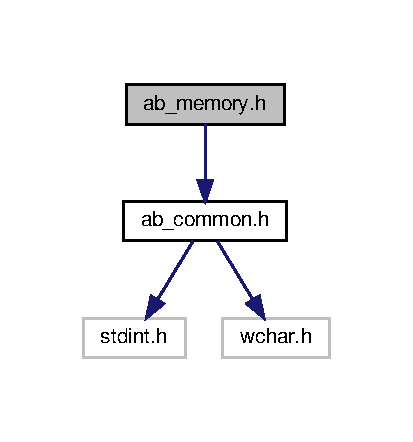
\includegraphics[width=198pt]{d7/d5f/ab__memory_8h__incl}
\end{center}
\end{figure}
This graph shows which files directly or indirectly include this file\+:\nopagebreak
\begin{figure}[H]
\begin{center}
\leavevmode
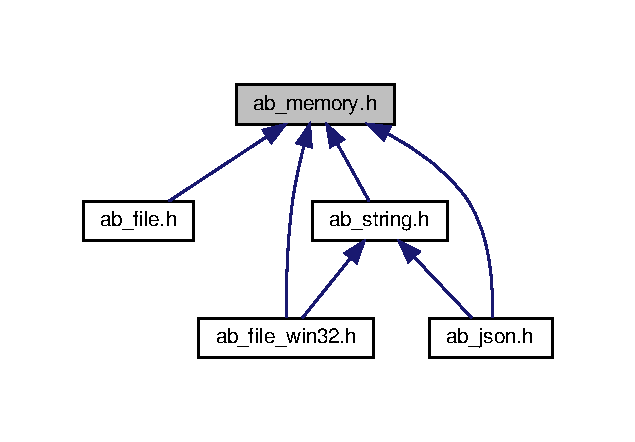
\includegraphics[width=350pt]{d4/d8c/ab__memory_8h__dep__incl}
\end{center}
\end{figure}
\subsection*{Classes}
\begin{DoxyCompactItemize}
\item 
struct \hyperlink{structmemory__arena}{memory\+\_\+arena}
\item 
struct \hyperlink{structtemporary__memory}{temporary\+\_\+memory}
\end{DoxyCompactItemize}
\subsection*{Macros}
\begin{DoxyCompactItemize}
\item 
\#define \hyperlink{ab__memory_8h_a0436d3ae4dac7362742c35ea6a146fea}{abm\+\_\+\+Push\+Struct}(Arena,  Type)~(Type$\ast$)\hyperlink{ab__memory_8h_a15270c8569eb858cdb20ee45c3bb46f7}{abm\+\_\+\+Push\+Size\+\_\+}(Arena, sizeof(Type))
\item 
\#define \hyperlink{ab__memory_8h_ab8d45b257f787efccb8a928176cc2c88}{abm\+\_\+\+Push\+Size}(Arena,  Size)~\hyperlink{ab__memory_8h_a15270c8569eb858cdb20ee45c3bb46f7}{abm\+\_\+\+Push\+Size\+\_\+}(Arena, Size)
\item 
\#define \hyperlink{ab__memory_8h_a89df166532e625eea593369a7997139d}{abm\+\_\+\+Push\+Array}(Arena,  Count,  Type)~(Type$\ast$)\hyperlink{ab__memory_8h_a15270c8569eb858cdb20ee45c3bb46f7}{abm\+\_\+\+Push\+Size\+\_\+}(Arena, (Count)$\ast$sizeof(Type))
\end{DoxyCompactItemize}
\subsection*{Functions}
\begin{DoxyCompactItemize}
\item 
void $\ast$ \hyperlink{ab__memory_8h_a20bffb2c2335745a56275b6094b6dcad}{abm\+\_\+\+Allocate\+Os\+Memory} (void $\ast$Address, size\+\_\+t Size)
\item 
void \hyperlink{ab__memory_8h_ad393d506412ba1d8d6fe25e8e16253b4}{abm\+\_\+\+Deallocate\+Os\+Memory} (void $\ast$Address, size\+\_\+t Size)
\item 
void $\ast$ \hyperlink{ab__memory_8h_a15270c8569eb858cdb20ee45c3bb46f7}{abm\+\_\+\+Push\+Size\+\_\+} (\hyperlink{structmemory__arena}{memory\+\_\+arena} $\ast$Memory, size\+\_\+t Size, \hyperlink{ab__common_8h_a70e369648385b50f2d0588e8e8745275}{b8} Clear\+Memory=true)
\item 
\hyperlink{structmemory__arena}{memory\+\_\+arena} \hyperlink{ab__memory_8h_a5f2fa70a405694492db91b26ed884207}{abm\+\_\+\+Init\+Memory} (void $\ast$Start, size\+\_\+t Size)
\item 
void \hyperlink{ab__memory_8h_a8ca432174a01c886b3c834cbb140c5ab}{abm\+\_\+\+Reset\+Memory} (\hyperlink{structmemory__arena}{memory\+\_\+arena} $\ast$Memory)
\item 
size\+\_\+t \hyperlink{ab__memory_8h_a9061bfb19b910033ab211832bc593fed}{abm\+\_\+\+Get\+Memory\+Left} (\hyperlink{structmemory__arena}{memory\+\_\+arena} $\ast$Memory)
\item 
\hyperlink{structtemporary__memory}{temporary\+\_\+memory} \hyperlink{ab__memory_8h_a77b6adde3ba40f7f3777bcc01c396ccd}{abm\+\_\+\+Begin\+Temporary\+Memory} (\hyperlink{structmemory__arena}{memory\+\_\+arena} $\ast$Memory)
\item 
void \hyperlink{ab__memory_8h_a8dbf22e067d85b9ad8422126755d23df}{abm\+\_\+\+End\+Temporary\+Memory} (\hyperlink{structtemporary__memory}{temporary\+\_\+memory} Temp\+Mem)
\item 
\hyperlink{structmemory__arena}{memory\+\_\+arena} \hyperlink{ab__memory_8h_a1b0ab8d04e6309ae31b1b2f8282dc085}{abm\+\_\+\+Create\+Sub\+Arena} (\hyperlink{structmemory__arena}{memory\+\_\+arena} $\ast$Memory, size\+\_\+t Size)
\end{DoxyCompactItemize}


\subsection{Macro Definition Documentation}
\mbox{\Hypertarget{ab__memory_8h_a89df166532e625eea593369a7997139d}\label{ab__memory_8h_a89df166532e625eea593369a7997139d}} 
\index{ab\+\_\+memory.\+h@{ab\+\_\+memory.\+h}!abm\+\_\+\+Push\+Array@{abm\+\_\+\+Push\+Array}}
\index{abm\+\_\+\+Push\+Array@{abm\+\_\+\+Push\+Array}!ab\+\_\+memory.\+h@{ab\+\_\+memory.\+h}}
\subsubsection{\texorpdfstring{abm\+\_\+\+Push\+Array}{abm\_PushArray}}
{\footnotesize\ttfamily \#define abm\+\_\+\+Push\+Array(\begin{DoxyParamCaption}\item[{}]{Arena,  }\item[{}]{Count,  }\item[{}]{Type }\end{DoxyParamCaption})~(Type$\ast$)\hyperlink{ab__memory_8h_a15270c8569eb858cdb20ee45c3bb46f7}{abm\+\_\+\+Push\+Size\+\_\+}(Arena, (Count)$\ast$sizeof(Type))}

\mbox{\Hypertarget{ab__memory_8h_ab8d45b257f787efccb8a928176cc2c88}\label{ab__memory_8h_ab8d45b257f787efccb8a928176cc2c88}} 
\index{ab\+\_\+memory.\+h@{ab\+\_\+memory.\+h}!abm\+\_\+\+Push\+Size@{abm\+\_\+\+Push\+Size}}
\index{abm\+\_\+\+Push\+Size@{abm\+\_\+\+Push\+Size}!ab\+\_\+memory.\+h@{ab\+\_\+memory.\+h}}
\subsubsection{\texorpdfstring{abm\+\_\+\+Push\+Size}{abm\_PushSize}}
{\footnotesize\ttfamily \#define abm\+\_\+\+Push\+Size(\begin{DoxyParamCaption}\item[{}]{Arena,  }\item[{}]{Size }\end{DoxyParamCaption})~\hyperlink{ab__memory_8h_a15270c8569eb858cdb20ee45c3bb46f7}{abm\+\_\+\+Push\+Size\+\_\+}(Arena, Size)}

\mbox{\Hypertarget{ab__memory_8h_a0436d3ae4dac7362742c35ea6a146fea}\label{ab__memory_8h_a0436d3ae4dac7362742c35ea6a146fea}} 
\index{ab\+\_\+memory.\+h@{ab\+\_\+memory.\+h}!abm\+\_\+\+Push\+Struct@{abm\+\_\+\+Push\+Struct}}
\index{abm\+\_\+\+Push\+Struct@{abm\+\_\+\+Push\+Struct}!ab\+\_\+memory.\+h@{ab\+\_\+memory.\+h}}
\subsubsection{\texorpdfstring{abm\+\_\+\+Push\+Struct}{abm\_PushStruct}}
{\footnotesize\ttfamily \#define abm\+\_\+\+Push\+Struct(\begin{DoxyParamCaption}\item[{}]{Arena,  }\item[{}]{Type }\end{DoxyParamCaption})~(Type$\ast$)\hyperlink{ab__memory_8h_a15270c8569eb858cdb20ee45c3bb46f7}{abm\+\_\+\+Push\+Size\+\_\+}(Arena, sizeof(Type))}



\subsection{Function Documentation}
\mbox{\Hypertarget{ab__memory_8h_a20bffb2c2335745a56275b6094b6dcad}\label{ab__memory_8h_a20bffb2c2335745a56275b6094b6dcad}} 
\index{ab\+\_\+memory.\+h@{ab\+\_\+memory.\+h}!abm\+\_\+\+Allocate\+Os\+Memory@{abm\+\_\+\+Allocate\+Os\+Memory}}
\index{abm\+\_\+\+Allocate\+Os\+Memory@{abm\+\_\+\+Allocate\+Os\+Memory}!ab\+\_\+memory.\+h@{ab\+\_\+memory.\+h}}
\subsubsection{\texorpdfstring{abm\+\_\+\+Allocate\+Os\+Memory()}{abm\_AllocateOsMemory()}}
{\footnotesize\ttfamily void$\ast$ abm\+\_\+\+Allocate\+Os\+Memory (\begin{DoxyParamCaption}\item[{void $\ast$}]{Address,  }\item[{size\+\_\+t}]{Size }\end{DoxyParamCaption})}

\mbox{\Hypertarget{ab__memory_8h_a77b6adde3ba40f7f3777bcc01c396ccd}\label{ab__memory_8h_a77b6adde3ba40f7f3777bcc01c396ccd}} 
\index{ab\+\_\+memory.\+h@{ab\+\_\+memory.\+h}!abm\+\_\+\+Begin\+Temporary\+Memory@{abm\+\_\+\+Begin\+Temporary\+Memory}}
\index{abm\+\_\+\+Begin\+Temporary\+Memory@{abm\+\_\+\+Begin\+Temporary\+Memory}!ab\+\_\+memory.\+h@{ab\+\_\+memory.\+h}}
\subsubsection{\texorpdfstring{abm\+\_\+\+Begin\+Temporary\+Memory()}{abm\_BeginTemporaryMemory()}}
{\footnotesize\ttfamily \hyperlink{structtemporary__memory}{temporary\+\_\+memory} abm\+\_\+\+Begin\+Temporary\+Memory (\begin{DoxyParamCaption}\item[{\hyperlink{structmemory__arena}{memory\+\_\+arena} $\ast$}]{Memory }\end{DoxyParamCaption})}

\mbox{\Hypertarget{ab__memory_8h_a1b0ab8d04e6309ae31b1b2f8282dc085}\label{ab__memory_8h_a1b0ab8d04e6309ae31b1b2f8282dc085}} 
\index{ab\+\_\+memory.\+h@{ab\+\_\+memory.\+h}!abm\+\_\+\+Create\+Sub\+Arena@{abm\+\_\+\+Create\+Sub\+Arena}}
\index{abm\+\_\+\+Create\+Sub\+Arena@{abm\+\_\+\+Create\+Sub\+Arena}!ab\+\_\+memory.\+h@{ab\+\_\+memory.\+h}}
\subsubsection{\texorpdfstring{abm\+\_\+\+Create\+Sub\+Arena()}{abm\_CreateSubArena()}}
{\footnotesize\ttfamily \hyperlink{structmemory__arena}{memory\+\_\+arena} abm\+\_\+\+Create\+Sub\+Arena (\begin{DoxyParamCaption}\item[{\hyperlink{structmemory__arena}{memory\+\_\+arena} $\ast$}]{Memory,  }\item[{size\+\_\+t}]{Size }\end{DoxyParamCaption})}

\mbox{\Hypertarget{ab__memory_8h_ad393d506412ba1d8d6fe25e8e16253b4}\label{ab__memory_8h_ad393d506412ba1d8d6fe25e8e16253b4}} 
\index{ab\+\_\+memory.\+h@{ab\+\_\+memory.\+h}!abm\+\_\+\+Deallocate\+Os\+Memory@{abm\+\_\+\+Deallocate\+Os\+Memory}}
\index{abm\+\_\+\+Deallocate\+Os\+Memory@{abm\+\_\+\+Deallocate\+Os\+Memory}!ab\+\_\+memory.\+h@{ab\+\_\+memory.\+h}}
\subsubsection{\texorpdfstring{abm\+\_\+\+Deallocate\+Os\+Memory()}{abm\_DeallocateOsMemory()}}
{\footnotesize\ttfamily void abm\+\_\+\+Deallocate\+Os\+Memory (\begin{DoxyParamCaption}\item[{void $\ast$}]{Address,  }\item[{size\+\_\+t}]{Size }\end{DoxyParamCaption})}

\mbox{\Hypertarget{ab__memory_8h_a8dbf22e067d85b9ad8422126755d23df}\label{ab__memory_8h_a8dbf22e067d85b9ad8422126755d23df}} 
\index{ab\+\_\+memory.\+h@{ab\+\_\+memory.\+h}!abm\+\_\+\+End\+Temporary\+Memory@{abm\+\_\+\+End\+Temporary\+Memory}}
\index{abm\+\_\+\+End\+Temporary\+Memory@{abm\+\_\+\+End\+Temporary\+Memory}!ab\+\_\+memory.\+h@{ab\+\_\+memory.\+h}}
\subsubsection{\texorpdfstring{abm\+\_\+\+End\+Temporary\+Memory()}{abm\_EndTemporaryMemory()}}
{\footnotesize\ttfamily void abm\+\_\+\+End\+Temporary\+Memory (\begin{DoxyParamCaption}\item[{\hyperlink{structtemporary__memory}{temporary\+\_\+memory}}]{Temp\+Mem }\end{DoxyParamCaption})}

\mbox{\Hypertarget{ab__memory_8h_a9061bfb19b910033ab211832bc593fed}\label{ab__memory_8h_a9061bfb19b910033ab211832bc593fed}} 
\index{ab\+\_\+memory.\+h@{ab\+\_\+memory.\+h}!abm\+\_\+\+Get\+Memory\+Left@{abm\+\_\+\+Get\+Memory\+Left}}
\index{abm\+\_\+\+Get\+Memory\+Left@{abm\+\_\+\+Get\+Memory\+Left}!ab\+\_\+memory.\+h@{ab\+\_\+memory.\+h}}
\subsubsection{\texorpdfstring{abm\+\_\+\+Get\+Memory\+Left()}{abm\_GetMemoryLeft()}}
{\footnotesize\ttfamily size\+\_\+t abm\+\_\+\+Get\+Memory\+Left (\begin{DoxyParamCaption}\item[{\hyperlink{structmemory__arena}{memory\+\_\+arena} $\ast$}]{Memory }\end{DoxyParamCaption})\hspace{0.3cm}{\ttfamily [inline]}}

\mbox{\Hypertarget{ab__memory_8h_a5f2fa70a405694492db91b26ed884207}\label{ab__memory_8h_a5f2fa70a405694492db91b26ed884207}} 
\index{ab\+\_\+memory.\+h@{ab\+\_\+memory.\+h}!abm\+\_\+\+Init\+Memory@{abm\+\_\+\+Init\+Memory}}
\index{abm\+\_\+\+Init\+Memory@{abm\+\_\+\+Init\+Memory}!ab\+\_\+memory.\+h@{ab\+\_\+memory.\+h}}
\subsubsection{\texorpdfstring{abm\+\_\+\+Init\+Memory()}{abm\_InitMemory()}}
{\footnotesize\ttfamily \hyperlink{structmemory__arena}{memory\+\_\+arena} abm\+\_\+\+Init\+Memory (\begin{DoxyParamCaption}\item[{void $\ast$}]{Start,  }\item[{size\+\_\+t}]{Size }\end{DoxyParamCaption})}

\mbox{\Hypertarget{ab__memory_8h_a15270c8569eb858cdb20ee45c3bb46f7}\label{ab__memory_8h_a15270c8569eb858cdb20ee45c3bb46f7}} 
\index{ab\+\_\+memory.\+h@{ab\+\_\+memory.\+h}!abm\+\_\+\+Push\+Size\+\_\+@{abm\+\_\+\+Push\+Size\+\_\+}}
\index{abm\+\_\+\+Push\+Size\+\_\+@{abm\+\_\+\+Push\+Size\+\_\+}!ab\+\_\+memory.\+h@{ab\+\_\+memory.\+h}}
\subsubsection{\texorpdfstring{abm\+\_\+\+Push\+Size\+\_\+()}{abm\_PushSize\_()}}
{\footnotesize\ttfamily void$\ast$ abm\+\_\+\+Push\+Size\+\_\+ (\begin{DoxyParamCaption}\item[{\hyperlink{structmemory__arena}{memory\+\_\+arena} $\ast$}]{Memory,  }\item[{size\+\_\+t}]{Size,  }\item[{\hyperlink{ab__common_8h_a70e369648385b50f2d0588e8e8745275}{b8}}]{Clear\+Memory = {\ttfamily true} }\end{DoxyParamCaption})}

\mbox{\Hypertarget{ab__memory_8h_a8ca432174a01c886b3c834cbb140c5ab}\label{ab__memory_8h_a8ca432174a01c886b3c834cbb140c5ab}} 
\index{ab\+\_\+memory.\+h@{ab\+\_\+memory.\+h}!abm\+\_\+\+Reset\+Memory@{abm\+\_\+\+Reset\+Memory}}
\index{abm\+\_\+\+Reset\+Memory@{abm\+\_\+\+Reset\+Memory}!ab\+\_\+memory.\+h@{ab\+\_\+memory.\+h}}
\subsubsection{\texorpdfstring{abm\+\_\+\+Reset\+Memory()}{abm\_ResetMemory()}}
{\footnotesize\ttfamily void abm\+\_\+\+Reset\+Memory (\begin{DoxyParamCaption}\item[{\hyperlink{structmemory__arena}{memory\+\_\+arena} $\ast$}]{Memory }\end{DoxyParamCaption})}


\hypertarget{ab__memory__linux_8h}{}\doxysection{ab\+\_\+memory\+\_\+linux.\+h File Reference}
\label{ab__memory__linux_8h}\index{ab\_memory\_linux.h@{ab\_memory\_linux.h}}


Linux specific implementation of some memory functions.  




\doxysubsection{Detailed Description}
Linux specific implementation of some memory functions. 

\begin{DoxyAuthor}{Author}
Amos Buchanan 
\end{DoxyAuthor}
\begin{DoxyVersion}{Version}
1.\+0 
\end{DoxyVersion}
\begin{DoxyDate}{Date}
2020 
\end{DoxyDate}
\begin{DoxyCopyright}{Copyright}
\href{https://opensource.org/licenses/MIT}{\texttt{ M\+IT Public License}}
\end{DoxyCopyright}
Linux specific implementation of functions. See \mbox{\hyperlink{ab__memory_8h}{ab\+\_\+memory.\+h}} for function usage. Do not include this file directly; it\textquotesingle{}s included from \mbox{\hyperlink{ab__memory_8h}{ab\+\_\+memory.\+h}} automatically.

\doxysubsection*{M\+IT License}

\href{https://opensource.org/licenses/MIT}{\texttt{ M\+IT Public License}}

Copyright 2020 Amos Buchanan

Permission is hereby granted, free of charge, to any person obtaining a copy of this software and associated documentation files (the \char`\"{}\+Software\char`\"{}), to deal in the Software without restriction, including without limitation the rights to use, copy, modify, merge, publish, distribute, sublicense, and/or sell copies of the Software, and to permit persons to whom the Software is furnished to do so, subject to the following conditions\+:

The above copyright notice and this permission notice shall be included in all copies or substantial portions of the Software.

T\+HE S\+O\+F\+T\+W\+A\+RE IS P\+R\+O\+V\+I\+D\+ED \char`\"{}\+A\+S I\+S\char`\"{}, W\+I\+T\+H\+O\+UT W\+A\+R\+R\+A\+N\+TY OF A\+NY K\+I\+ND, E\+X\+P\+R\+E\+SS OR I\+M\+P\+L\+I\+ED, I\+N\+C\+L\+U\+D\+I\+NG B\+UT N\+OT L\+I\+M\+I\+T\+ED TO T\+HE W\+A\+R\+R\+A\+N\+T\+I\+ES OF M\+E\+R\+C\+H\+A\+N\+T\+A\+B\+I\+L\+I\+TY, F\+I\+T\+N\+E\+SS F\+OR A P\+A\+R\+T\+I\+C\+U\+L\+AR P\+U\+R\+P\+O\+SE A\+ND N\+O\+N\+I\+N\+F\+R\+I\+N\+G\+E\+M\+E\+NT. IN NO E\+V\+E\+NT S\+H\+A\+LL T\+HE A\+U\+T\+H\+O\+RS OR C\+O\+P\+Y\+R\+I\+G\+HT H\+O\+L\+D\+E\+RS BE L\+I\+A\+B\+LE F\+OR A\+NY C\+L\+A\+IM, D\+A\+M\+A\+G\+ES OR O\+T\+H\+ER L\+I\+A\+B\+I\+L\+I\+TY, W\+H\+E\+T\+H\+ER IN AN A\+C\+T\+I\+ON OF C\+O\+N\+T\+R\+A\+CT, T\+O\+RT OR O\+T\+H\+E\+R\+W\+I\+SE, A\+R\+I\+S\+I\+NG F\+R\+OM, O\+UT OF OR IN C\+O\+N\+N\+E\+C\+T\+I\+ON W\+I\+TH T\+HE S\+O\+F\+T\+W\+A\+RE OR T\+HE U\+SE OR O\+T\+H\+ER D\+E\+A\+L\+I\+N\+GS IN T\+HE S\+O\+F\+T\+W\+A\+RE. 
\hypertarget{ab__memory__win32_8h}{}\doxysection{ab\+\_\+memory\+\_\+win32.\+h File Reference}
\label{ab__memory__win32_8h}\index{ab\_memory\_win32.h@{ab\_memory\_win32.h}}


Windows specific implementation of some memory functions.  




\doxysubsection{Detailed Description}
Windows specific implementation of some memory functions. 

\begin{DoxyAuthor}{Author}
Amos Buchanan 
\end{DoxyAuthor}
\begin{DoxyVersion}{Version}
1.\+0 
\end{DoxyVersion}
\begin{DoxyDate}{Date}
2020
\end{DoxyDate}
Windows specific implementation of functions. See \mbox{\hyperlink{ab__memory_8h}{ab\+\_\+memory.\+h}} for function usage. Do not include this file directly; it\textquotesingle{}s included from \mbox{\hyperlink{ab__memory_8h}{ab\+\_\+memory.\+h}} automatically. 
\hypertarget{ab__string_8h}{}\doxysection{ab\+\_\+string.\+h File Reference}
\label{ab__string_8h}\index{ab\_string.h@{ab\_string.h}}


Using string fragments, usually but not exclusively sections of larger strings.  


{\ttfamily \#include \char`\"{}ab\+\_\+memory.\+h\char`\"{}}\newline
Include dependency graph for ab\+\_\+string.\+h\+:\nopagebreak
\begin{figure}[H]
\begin{center}
\leavevmode
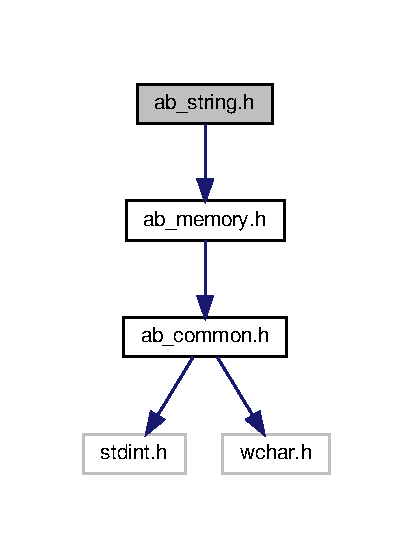
\includegraphics[width=198pt]{de/dc1/ab__string_8h__incl}
\end{center}
\end{figure}
This graph shows which files directly or indirectly include this file\+:\nopagebreak
\begin{figure}[H]
\begin{center}
\leavevmode
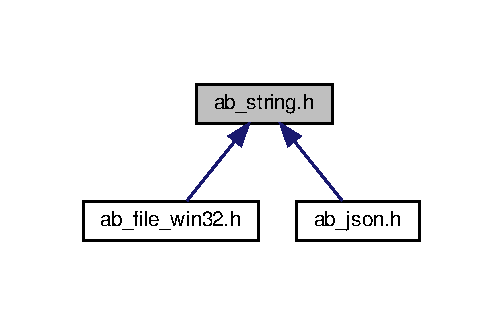
\includegraphics[width=145pt]{df/d7f/ab__string_8h__dep__incl}
\end{center}
\end{figure}
\doxysubsection*{Classes}
\begin{DoxyCompactItemize}
\item 
struct \mbox{\hyperlink{structst__ptr}{st\+\_\+ptr}}
\begin{DoxyCompactList}\small\item\em Pointer and length of a character array. \end{DoxyCompactList}\end{DoxyCompactItemize}
\doxysubsection*{Macros}
\begin{DoxyCompactItemize}
\item 
\#define \mbox{\hyperlink{ab__string_8h_a7f78f576bc59e91ba524ecacde27fb02}{P\+S\+T\+R\+I\+NG}}(S\+TR)~S\+T\+R.\+Length, S\+T\+R.\+String
\begin{DoxyCompactList}\small\item\em Helper to print \mbox{\hyperlink{structst__ptr}{st\+\_\+ptr}}. \end{DoxyCompactList}\end{DoxyCompactItemize}
\doxysubsection*{Functions}
\begin{DoxyCompactItemize}
\item 
\mbox{\hyperlink{ab__common_8h_afaa62991928fb9fb18ff0db62a040aba}{u32}} \mbox{\hyperlink{ab__string_8h_ac07424bcd3602591f8421bed6ca226cc}{st\+\_\+\+String\+Length}} (char const $\ast$x, \mbox{\hyperlink{ab__common_8h_afaa62991928fb9fb18ff0db62a040aba}{u32}} Max\+Length)
\begin{DoxyCompactList}\small\item\em Get the length of a null-\/terminated string. \end{DoxyCompactList}\item 
\mbox{\hyperlink{ab__common_8h_a70e369648385b50f2d0588e8e8745275}{b8}} \mbox{\hyperlink{ab__string_8h_ac86287d9d07821dfc6b740f0ebc03e7d}{st\+\_\+\+Are\+Strings\+Equal}} (char const $\ast$String1, char const $\ast$String2, \mbox{\hyperlink{ab__common_8h_afaa62991928fb9fb18ff0db62a040aba}{u32}} Max\+Length, \mbox{\hyperlink{ab__common_8h_a70e369648385b50f2d0588e8e8745275}{b8}} is\+Case\+Insensitive)
\begin{DoxyCompactList}\small\item\em Compare two strings. \end{DoxyCompactList}\item 
\mbox{\hyperlink{ab__common_8h_a70e369648385b50f2d0588e8e8745275}{b8}} \mbox{\hyperlink{ab__string_8h_ab3cb2a132e3a3b4e219bb2242a94928f}{st\+\_\+\+Are\+Strings\+Equal}} (const char $\ast$String1, \mbox{\hyperlink{ab__common_8h_afaa62991928fb9fb18ff0db62a040aba}{u32}} String1\+Len, const char $\ast$String2, \mbox{\hyperlink{ab__common_8h_afaa62991928fb9fb18ff0db62a040aba}{u32}} String2\+Len, \mbox{\hyperlink{ab__common_8h_a70e369648385b50f2d0588e8e8745275}{b8}} is\+Case\+Insensitive)
\begin{DoxyCompactList}\small\item\em Compare two strings. \end{DoxyCompactList}\item 
\mbox{\hyperlink{ab__common_8h_a70e369648385b50f2d0588e8e8745275}{b8}} \mbox{\hyperlink{ab__string_8h_a71d738c82a030990ac4cd11228187aed}{st\+\_\+\+Are\+Strings\+Equal}} (char const $\ast$String1, \mbox{\hyperlink{ab__common_8h_afaa62991928fb9fb18ff0db62a040aba}{u32}} String1\+Len, char const $\ast$String2, \mbox{\hyperlink{ab__common_8h_afaa62991928fb9fb18ff0db62a040aba}{u32}} String2\+Len)
\begin{DoxyCompactList}\small\item\em Compare two strings. \end{DoxyCompactList}\item 
\mbox{\hyperlink{ab__common_8h_a70e369648385b50f2d0588e8e8745275}{b8}} \mbox{\hyperlink{ab__string_8h_a1933d349d4f32a3b49e5f4364a56b4e6}{st\+\_\+\+Are\+Strings\+Equal}} (\mbox{\hyperlink{structst__ptr}{st\+\_\+ptr}} String1, \mbox{\hyperlink{structst__ptr}{st\+\_\+ptr}} String2)
\begin{DoxyCompactList}\small\item\em Compare two {\ttfamily \mbox{\hyperlink{structst__ptr}{st\+\_\+ptr}}}. \end{DoxyCompactList}\item 
\mbox{\hyperlink{ab__common_8h_a70e369648385b50f2d0588e8e8745275}{b8}} \mbox{\hyperlink{ab__string_8h_a0a7381b99009fa1cd3ecd46cf5de2c88}{st\+\_\+\+Are\+Strings\+Equal}} (char const $\ast$String, \mbox{\hyperlink{ab__common_8h_afaa62991928fb9fb18ff0db62a040aba}{u32}} String\+Len, \mbox{\hyperlink{structst__ptr}{st\+\_\+ptr}} String\+Ptr)
\begin{DoxyCompactList}\small\item\em Compare a null-\/terminated string with a {\ttfamily \mbox{\hyperlink{structst__ptr}{st\+\_\+ptr}}}. \end{DoxyCompactList}\item 
\mbox{\hyperlink{ab__common_8h_ae9b1af5c037e57a98884758875d3a7c4}{s32}} \mbox{\hyperlink{ab__string_8h_a1a043a15b730b8d058445c28cede1906}{st\+\_\+\+Find\+In\+List}} (\mbox{\hyperlink{structst__ptr}{st\+\_\+ptr}} String, \mbox{\hyperlink{ab__common_8h_afaa62991928fb9fb18ff0db62a040aba}{u32}} List\+Count, const \mbox{\hyperlink{structst__ptr}{st\+\_\+ptr}} $\ast$List, \mbox{\hyperlink{ab__common_8h_a70e369648385b50f2d0588e8e8745275}{b8}} is\+Case\+Insensitive=false)
\begin{DoxyCompactList}\small\item\em Find a string in a list of strings. \end{DoxyCompactList}\item 
\mbox{\hyperlink{ab__common_8h_ae9b1af5c037e57a98884758875d3a7c4}{s32}} \mbox{\hyperlink{ab__string_8h_a988b3993f14543652378ae4b915e1e15}{st\+\_\+\+Find\+In\+List}} (const char $\ast$Search\+String, \mbox{\hyperlink{ab__common_8h_afaa62991928fb9fb18ff0db62a040aba}{u32}} List\+Count, const \mbox{\hyperlink{structst__ptr}{st\+\_\+ptr}} $\ast$List, \mbox{\hyperlink{ab__common_8h_a70e369648385b50f2d0588e8e8745275}{b8}} is\+Case\+Insensitive=false)
\begin{DoxyCompactList}\small\item\em Find a string in a list of strings. \end{DoxyCompactList}\item 
\mbox{\hyperlink{ab__common_8h_afaa62991928fb9fb18ff0db62a040aba}{u32}} \mbox{\hyperlink{ab__string_8h_a3bb4db362b23466a8a4ec56f4cc82816}{st\+\_\+\+String\+Copy}} (char $\ast$Dest\+String, const char $\ast$Src\+String, size\+\_\+t Length, \mbox{\hyperlink{ab__common_8h_a70e369648385b50f2d0588e8e8745275}{b8}} Add\+Terminator)
\begin{DoxyCompactList}\small\item\em Safe null-\/terminated string copy. \end{DoxyCompactList}\item 
\mbox{\hyperlink{structst__ptr}{st\+\_\+ptr}} \mbox{\hyperlink{ab__string_8h_a954364e0fd13aaca0011607310d8b455}{st\+\_\+\+Create\+String\+Ptr}} (memory\+\_\+arena $\ast$Memory, const char $\ast$String)
\begin{DoxyCompactList}\small\item\em Create a string pointer out of a string. \end{DoxyCompactList}\item 
\mbox{\hyperlink{structst__ptr}{st\+\_\+ptr}} \mbox{\hyperlink{ab__string_8h_acca3ec335b387116dc3bae074f9655d1}{Create\+String\+Ptr}} (char const $\ast$String, \mbox{\hyperlink{ab__common_8h_afaa62991928fb9fb18ff0db62a040aba}{u32}} Length)
\begin{DoxyCompactList}\small\item\em Create a string pointer out of a constant string. \end{DoxyCompactList}\end{DoxyCompactItemize}


\doxysubsection{Detailed Description}
Using string fragments, usually but not exclusively sections of larger strings. 

\begin{DoxyAuthor}{Author}
Amos Buchanan 
\end{DoxyAuthor}
\begin{DoxyVersion}{Version}
1.\+0 
\end{DoxyVersion}
\begin{DoxyDate}{Date}
2020
\end{DoxyDate}
These are functions to handle string fragments. There are also some safe string copy and find functions. {\ttfamily \mbox{\hyperlink{structst__ptr}{st\+\_\+ptr}}} is generally used for a fragment of a larger piece of text.

This is a single-\/file library. You may include it as a header just as any other. Add the following define to include the source {\itshape once} per project\+:


\begin{DoxyCode}{0}
\DoxyCodeLine{\textcolor{preprocessor}{\#define STRING\_SRC}}
\DoxyCodeLine{\textcolor{preprocessor}{\#include "{}ab\_string.h"{}}}
\end{DoxyCode}
 

\doxysubsection{Macro Definition Documentation}
\mbox{\Hypertarget{ab__string_8h_a7f78f576bc59e91ba524ecacde27fb02}\label{ab__string_8h_a7f78f576bc59e91ba524ecacde27fb02}} 
\index{ab\_string.h@{ab\_string.h}!PSTRING@{PSTRING}}
\index{PSTRING@{PSTRING}!ab\_string.h@{ab\_string.h}}
\doxysubsubsection{\texorpdfstring{PSTRING}{PSTRING}}
{\footnotesize\ttfamily \#define P\+S\+T\+R\+I\+NG(\begin{DoxyParamCaption}\item[{}]{S\+TR }\end{DoxyParamCaption})~S\+T\+R.\+Length, S\+T\+R.\+String}



Helper to print \mbox{\hyperlink{structst__ptr}{st\+\_\+ptr}}. 

Used for input to $\ast$printf() type functions.

Example Usage\+: 
\begin{DoxyCode}{0}
\DoxyCodeLine{\mbox{\hyperlink{structst__ptr}{st\_ptr}} AString = \textcolor{stringliteral}{"{}SomeString"{}};}
\DoxyCodeLine{printf(\textcolor{stringliteral}{"{}String: \%.*s"{}}, \mbox{\hyperlink{ab__string_8h_a7f78f576bc59e91ba524ecacde27fb02}{PSTRING}}(AString));}
\end{DoxyCode}



\begin{DoxyParams}{Parameters}
{\em S\+TR} & A \mbox{\hyperlink{structst__ptr}{st\+\_\+ptr}} object. \\
\hline
\end{DoxyParams}


\doxysubsection{Function Documentation}
\mbox{\Hypertarget{ab__string_8h_acca3ec335b387116dc3bae074f9655d1}\label{ab__string_8h_acca3ec335b387116dc3bae074f9655d1}} 
\index{ab\_string.h@{ab\_string.h}!CreateStringPtr@{CreateStringPtr}}
\index{CreateStringPtr@{CreateStringPtr}!ab\_string.h@{ab\_string.h}}
\doxysubsubsection{\texorpdfstring{CreateStringPtr()}{CreateStringPtr()}}
{\footnotesize\ttfamily \mbox{\hyperlink{structst__ptr}{st\+\_\+ptr}} Create\+String\+Ptr (\begin{DoxyParamCaption}\item[{char const $\ast$}]{String,  }\item[{\mbox{\hyperlink{ab__common_8h_afaa62991928fb9fb18ff0db62a040aba}{u32}}}]{Length }\end{DoxyParamCaption})}



Create a string pointer out of a constant string. 


\begin{DoxyParams}{Parameters}
{\em String} & Null terminated const string. \\
\hline
{\em Length} & Length of the string. \\
\hline
\end{DoxyParams}
\begin{DoxyReturn}{Returns}
\mbox{\hyperlink{structst__ptr}{st\+\_\+ptr}} to the existing string using length. 
\end{DoxyReturn}
\mbox{\Hypertarget{ab__string_8h_a0a7381b99009fa1cd3ecd46cf5de2c88}\label{ab__string_8h_a0a7381b99009fa1cd3ecd46cf5de2c88}} 
\index{ab\_string.h@{ab\_string.h}!st\_AreStringsEqual@{st\_AreStringsEqual}}
\index{st\_AreStringsEqual@{st\_AreStringsEqual}!ab\_string.h@{ab\_string.h}}
\doxysubsubsection{\texorpdfstring{st\_AreStringsEqual()}{st\_AreStringsEqual()}\hspace{0.1cm}{\footnotesize\ttfamily [1/5]}}
{\footnotesize\ttfamily \mbox{\hyperlink{ab__common_8h_a70e369648385b50f2d0588e8e8745275}{b8}} st\+\_\+\+Are\+Strings\+Equal (\begin{DoxyParamCaption}\item[{char const $\ast$}]{String,  }\item[{\mbox{\hyperlink{ab__common_8h_afaa62991928fb9fb18ff0db62a040aba}{u32}}}]{String\+Len,  }\item[{\mbox{\hyperlink{structst__ptr}{st\+\_\+ptr}}}]{String\+Ptr }\end{DoxyParamCaption})}



Compare a null-\/terminated string with a {\ttfamily \mbox{\hyperlink{structst__ptr}{st\+\_\+ptr}}}. 

Case sensitive comparison of null-\/terminated string and {\ttfamily \mbox{\hyperlink{structst__ptr}{st\+\_\+ptr}}}.


\begin{DoxyParams}{Parameters}
{\em String} & Null terminated string. \\
\hline
{\em String\+Len} & Maximum length of null terminated string to check. \\
\hline
{\em String\+Ptr} & Second string to check. \\
\hline
\end{DoxyParams}
\begin{DoxyReturn}{Returns}
True if strings are equal, including lengths. False if strings are unequal, or if one is null-\/terminated before the other. 
\end{DoxyReturn}
\mbox{\Hypertarget{ab__string_8h_ac86287d9d07821dfc6b740f0ebc03e7d}\label{ab__string_8h_ac86287d9d07821dfc6b740f0ebc03e7d}} 
\index{ab\_string.h@{ab\_string.h}!st\_AreStringsEqual@{st\_AreStringsEqual}}
\index{st\_AreStringsEqual@{st\_AreStringsEqual}!ab\_string.h@{ab\_string.h}}
\doxysubsubsection{\texorpdfstring{st\_AreStringsEqual()}{st\_AreStringsEqual()}\hspace{0.1cm}{\footnotesize\ttfamily [2/5]}}
{\footnotesize\ttfamily \mbox{\hyperlink{ab__common_8h_a70e369648385b50f2d0588e8e8745275}{b8}} st\+\_\+\+Are\+Strings\+Equal (\begin{DoxyParamCaption}\item[{char const $\ast$}]{String1,  }\item[{char const $\ast$}]{String2,  }\item[{\mbox{\hyperlink{ab__common_8h_afaa62991928fb9fb18ff0db62a040aba}{u32}}}]{Max\+Length,  }\item[{\mbox{\hyperlink{ab__common_8h_a70e369648385b50f2d0588e8e8745275}{b8}}}]{is\+Case\+Insensitive }\end{DoxyParamCaption})}



Compare two strings. 


\begin{DoxyParams}{Parameters}
{\em String1} & Null terminated c-\/string. \\
\hline
{\em String2} & Null terminated c-\/string. \\
\hline
{\em Max\+Length} & Maximum number of characters to check. \\
\hline
{\em is\+Case\+Insensitive} & True for case insensitive search. \\
\hline
\end{DoxyParams}
\begin{DoxyReturn}{Returns}
True if strings are equal, up to Max\+Length. False if strings are unequal, or if one is null-\/terminated before the other. 
\end{DoxyReturn}
\mbox{\Hypertarget{ab__string_8h_a71d738c82a030990ac4cd11228187aed}\label{ab__string_8h_a71d738c82a030990ac4cd11228187aed}} 
\index{ab\_string.h@{ab\_string.h}!st\_AreStringsEqual@{st\_AreStringsEqual}}
\index{st\_AreStringsEqual@{st\_AreStringsEqual}!ab\_string.h@{ab\_string.h}}
\doxysubsubsection{\texorpdfstring{st\_AreStringsEqual()}{st\_AreStringsEqual()}\hspace{0.1cm}{\footnotesize\ttfamily [3/5]}}
{\footnotesize\ttfamily \mbox{\hyperlink{ab__common_8h_a70e369648385b50f2d0588e8e8745275}{b8}} st\+\_\+\+Are\+Strings\+Equal (\begin{DoxyParamCaption}\item[{char const $\ast$}]{String1,  }\item[{\mbox{\hyperlink{ab__common_8h_afaa62991928fb9fb18ff0db62a040aba}{u32}}}]{String1\+Len,  }\item[{char const $\ast$}]{String2,  }\item[{\mbox{\hyperlink{ab__common_8h_afaa62991928fb9fb18ff0db62a040aba}{u32}}}]{String2\+Len }\end{DoxyParamCaption})}



Compare two strings. 

Case sensitive comparison, otherwise same as {\ttfamily \mbox{\hyperlink{ab__string_8h_ab3cb2a132e3a3b4e219bb2242a94928f}{st\+\_\+\+Are\+Strings\+Equal(const char $\ast$\+String1, u32 String1\+Len, const char $\ast$\+String2, u32 String2\+Len, b8 is\+Case\+Insensitive)}}}.


\begin{DoxyParams}{Parameters}
{\em String1} & Null terminated c-\/string. \\
\hline
{\em String1\+Len} & Length of string 1. \\
\hline
{\em String2} & Null terminated c-\/string. \\
\hline
{\em String2\+Len} & Length of string 2. \\
\hline
\end{DoxyParams}
\begin{DoxyReturn}{Returns}
True if strings are equal, including lengths. False if strings are unequal, or if one is null-\/terminated before the other. 
\end{DoxyReturn}
\mbox{\Hypertarget{ab__string_8h_ab3cb2a132e3a3b4e219bb2242a94928f}\label{ab__string_8h_ab3cb2a132e3a3b4e219bb2242a94928f}} 
\index{ab\_string.h@{ab\_string.h}!st\_AreStringsEqual@{st\_AreStringsEqual}}
\index{st\_AreStringsEqual@{st\_AreStringsEqual}!ab\_string.h@{ab\_string.h}}
\doxysubsubsection{\texorpdfstring{st\_AreStringsEqual()}{st\_AreStringsEqual()}\hspace{0.1cm}{\footnotesize\ttfamily [4/5]}}
{\footnotesize\ttfamily \mbox{\hyperlink{ab__common_8h_a70e369648385b50f2d0588e8e8745275}{b8}} st\+\_\+\+Are\+Strings\+Equal (\begin{DoxyParamCaption}\item[{const char $\ast$}]{String1,  }\item[{\mbox{\hyperlink{ab__common_8h_afaa62991928fb9fb18ff0db62a040aba}{u32}}}]{String1\+Len,  }\item[{const char $\ast$}]{String2,  }\item[{\mbox{\hyperlink{ab__common_8h_afaa62991928fb9fb18ff0db62a040aba}{u32}}}]{String2\+Len,  }\item[{\mbox{\hyperlink{ab__common_8h_a70e369648385b50f2d0588e8e8745275}{b8}}}]{is\+Case\+Insensitive }\end{DoxyParamCaption})}



Compare two strings. 

Compares 2 null-\/terminated strings, up to each length. False if strings are unequal, or one terminates before the other.


\begin{DoxyParams}{Parameters}
{\em String1} & Null terminated c-\/string. \\
\hline
{\em String1\+Len} & Length of string 1. \\
\hline
{\em String2} & Null terminated c-\/string. \\
\hline
{\em String2\+Len} & Length of string 2. \\
\hline
{\em is\+Case\+Insensitive} & True for case insensitive search. \\
\hline
\end{DoxyParams}
\begin{DoxyReturn}{Returns}
True if strings are equal, including lengths. False if strings are unequal, or if one is null-\/terminated before the other. 
\end{DoxyReturn}
\mbox{\Hypertarget{ab__string_8h_a1933d349d4f32a3b49e5f4364a56b4e6}\label{ab__string_8h_a1933d349d4f32a3b49e5f4364a56b4e6}} 
\index{ab\_string.h@{ab\_string.h}!st\_AreStringsEqual@{st\_AreStringsEqual}}
\index{st\_AreStringsEqual@{st\_AreStringsEqual}!ab\_string.h@{ab\_string.h}}
\doxysubsubsection{\texorpdfstring{st\_AreStringsEqual()}{st\_AreStringsEqual()}\hspace{0.1cm}{\footnotesize\ttfamily [5/5]}}
{\footnotesize\ttfamily \mbox{\hyperlink{ab__common_8h_a70e369648385b50f2d0588e8e8745275}{b8}} st\+\_\+\+Are\+Strings\+Equal (\begin{DoxyParamCaption}\item[{\mbox{\hyperlink{structst__ptr}{st\+\_\+ptr}}}]{String1,  }\item[{\mbox{\hyperlink{structst__ptr}{st\+\_\+ptr}}}]{String2 }\end{DoxyParamCaption})}



Compare two {\ttfamily \mbox{\hyperlink{structst__ptr}{st\+\_\+ptr}}}. 

Case sensitive comparison of two {\ttfamily \mbox{\hyperlink{structst__ptr}{st\+\_\+ptr}}}.


\begin{DoxyParams}{Parameters}
{\em String1} & String or string fragment. May not be null-\/terminated. \\
\hline
{\em String2} & String or string fragment. May not be null-\/terminated. \\
\hline
\end{DoxyParams}
\begin{DoxyReturn}{Returns}
True if strings are equal, including lengths. False if strings are unequal. 
\end{DoxyReturn}
\mbox{\Hypertarget{ab__string_8h_a954364e0fd13aaca0011607310d8b455}\label{ab__string_8h_a954364e0fd13aaca0011607310d8b455}} 
\index{ab\_string.h@{ab\_string.h}!st\_CreateStringPtr@{st\_CreateStringPtr}}
\index{st\_CreateStringPtr@{st\_CreateStringPtr}!ab\_string.h@{ab\_string.h}}
\doxysubsubsection{\texorpdfstring{st\_CreateStringPtr()}{st\_CreateStringPtr()}}
{\footnotesize\ttfamily \mbox{\hyperlink{structst__ptr}{st\+\_\+ptr}} st\+\_\+\+Create\+String\+Ptr (\begin{DoxyParamCaption}\item[{memory\+\_\+arena $\ast$}]{Memory,  }\item[{const char $\ast$}]{String }\end{DoxyParamCaption})}



Create a string pointer out of a string. 


\begin{DoxyParams}{Parameters}
{\em Memory} & Memory to use for the string. \\
\hline
{\em String} & Null terminated string to copy. \\
\hline
\end{DoxyParams}
\begin{DoxyReturn}{Returns}
\mbox{\hyperlink{structst__ptr}{st\+\_\+ptr}} to a new string. 
\end{DoxyReturn}
\mbox{\Hypertarget{ab__string_8h_a988b3993f14543652378ae4b915e1e15}\label{ab__string_8h_a988b3993f14543652378ae4b915e1e15}} 
\index{ab\_string.h@{ab\_string.h}!st\_FindInList@{st\_FindInList}}
\index{st\_FindInList@{st\_FindInList}!ab\_string.h@{ab\_string.h}}
\doxysubsubsection{\texorpdfstring{st\_FindInList()}{st\_FindInList()}\hspace{0.1cm}{\footnotesize\ttfamily [1/2]}}
{\footnotesize\ttfamily \mbox{\hyperlink{ab__common_8h_ae9b1af5c037e57a98884758875d3a7c4}{s32}} st\+\_\+\+Find\+In\+List (\begin{DoxyParamCaption}\item[{const char $\ast$}]{Search\+String,  }\item[{\mbox{\hyperlink{ab__common_8h_afaa62991928fb9fb18ff0db62a040aba}{u32}}}]{List\+Count,  }\item[{const \mbox{\hyperlink{structst__ptr}{st\+\_\+ptr}} $\ast$}]{List,  }\item[{\mbox{\hyperlink{ab__common_8h_a70e369648385b50f2d0588e8e8745275}{b8}}}]{is\+Case\+Insensitive = {\ttfamily false} }\end{DoxyParamCaption})}



Find a string in a list of strings. 


\begin{DoxyParams}{Parameters}
{\em Search\+String} & Null terminated string to search for. \\
\hline
{\em List\+Count} & Number of items in the list. \\
\hline
{\em List} & Pointer to the first item in the list. \\
\hline
{\em is\+Case\+Insensitive} & True if case insensitive, defaults to false. \\
\hline
\end{DoxyParams}
\begin{DoxyReturn}{Returns}
Index of the matching item, or -\/1 if no match found. 
\end{DoxyReturn}
\mbox{\Hypertarget{ab__string_8h_a1a043a15b730b8d058445c28cede1906}\label{ab__string_8h_a1a043a15b730b8d058445c28cede1906}} 
\index{ab\_string.h@{ab\_string.h}!st\_FindInList@{st\_FindInList}}
\index{st\_FindInList@{st\_FindInList}!ab\_string.h@{ab\_string.h}}
\doxysubsubsection{\texorpdfstring{st\_FindInList()}{st\_FindInList()}\hspace{0.1cm}{\footnotesize\ttfamily [2/2]}}
{\footnotesize\ttfamily \mbox{\hyperlink{ab__common_8h_ae9b1af5c037e57a98884758875d3a7c4}{s32}} st\+\_\+\+Find\+In\+List (\begin{DoxyParamCaption}\item[{\mbox{\hyperlink{structst__ptr}{st\+\_\+ptr}}}]{String,  }\item[{\mbox{\hyperlink{ab__common_8h_afaa62991928fb9fb18ff0db62a040aba}{u32}}}]{List\+Count,  }\item[{const \mbox{\hyperlink{structst__ptr}{st\+\_\+ptr}} $\ast$}]{List,  }\item[{\mbox{\hyperlink{ab__common_8h_a70e369648385b50f2d0588e8e8745275}{b8}}}]{is\+Case\+Insensitive = {\ttfamily false} }\end{DoxyParamCaption})}



Find a string in a list of strings. 


\begin{DoxyParams}{Parameters}
{\em String} & String to search for. \\
\hline
{\em List\+Count} & Number of items in the list. \\
\hline
{\em List} & Pointer to the first item in the list. \\
\hline
{\em is\+Case\+Insensitive} & True if case insensitive, defaults to false. \\
\hline
\end{DoxyParams}
\begin{DoxyReturn}{Returns}
Index of the matching item, or -\/1 if no match found. 
\end{DoxyReturn}
\mbox{\Hypertarget{ab__string_8h_a3bb4db362b23466a8a4ec56f4cc82816}\label{ab__string_8h_a3bb4db362b23466a8a4ec56f4cc82816}} 
\index{ab\_string.h@{ab\_string.h}!st\_StringCopy@{st\_StringCopy}}
\index{st\_StringCopy@{st\_StringCopy}!ab\_string.h@{ab\_string.h}}
\doxysubsubsection{\texorpdfstring{st\_StringCopy()}{st\_StringCopy()}}
{\footnotesize\ttfamily \mbox{\hyperlink{ab__common_8h_afaa62991928fb9fb18ff0db62a040aba}{u32}} st\+\_\+\+String\+Copy (\begin{DoxyParamCaption}\item[{char $\ast$}]{Dest\+String,  }\item[{const char $\ast$}]{Src\+String,  }\item[{size\+\_\+t}]{Length,  }\item[{\mbox{\hyperlink{ab__common_8h_a70e369648385b50f2d0588e8e8745275}{b8}}}]{Add\+Terminator }\end{DoxyParamCaption})}



Safe null-\/terminated string copy. 


\begin{DoxyParams}[1]{Parameters}
\mbox{\texttt{ out}}  & {\em Dest\+String} & Destination Buffer. \\
\hline
 & {\em Src\+String} & Source Buffer. \\
\hline
 & {\em Length} & Maximum length of Destination buffer. \\
\hline
 & {\em Add\+Terminator} & True to add a null terminator to the destination string. \\
\hline
\end{DoxyParams}
\begin{DoxyReturn}{Returns}
Number of characters copied. 
\end{DoxyReturn}
\mbox{\Hypertarget{ab__string_8h_ac07424bcd3602591f8421bed6ca226cc}\label{ab__string_8h_ac07424bcd3602591f8421bed6ca226cc}} 
\index{ab\_string.h@{ab\_string.h}!st\_StringLength@{st\_StringLength}}
\index{st\_StringLength@{st\_StringLength}!ab\_string.h@{ab\_string.h}}
\doxysubsubsection{\texorpdfstring{st\_StringLength()}{st\_StringLength()}}
{\footnotesize\ttfamily \mbox{\hyperlink{ab__common_8h_afaa62991928fb9fb18ff0db62a040aba}{u32}} st\+\_\+\+String\+Length (\begin{DoxyParamCaption}\item[{char const $\ast$}]{x,  }\item[{\mbox{\hyperlink{ab__common_8h_afaa62991928fb9fb18ff0db62a040aba}{u32}}}]{Max\+Length }\end{DoxyParamCaption})}



Get the length of a null-\/terminated string. 


\begin{DoxyParams}{Parameters}
{\em x} & C-\/style string. \\
\hline
{\em Max\+Length} & Maximum length to check. \\
\hline
\end{DoxyParams}
\begin{DoxyReturn}{Returns}
Length of string, or Max\+Length if no null termination before then. 
\end{DoxyReturn}

\hypertarget{ab__time_8h}{}\section{ab\+\_\+time.\+h File Reference}
\label{ab__time_8h}\index{ab\+\_\+time.\+h@{ab\+\_\+time.\+h}}
{\ttfamily \#include $<$time.\+h$>$}\newline
{\ttfamily \#include \char`\"{}ab\+\_\+common.\+h\char`\"{}}\newline
Include dependency graph for ab\+\_\+time.\+h\+:\nopagebreak
\begin{figure}[H]
\begin{center}
\leavevmode
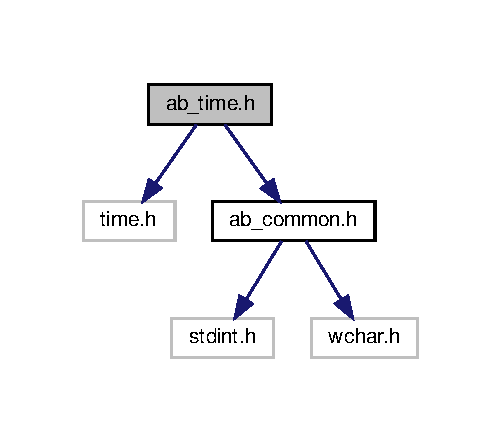
\includegraphics[width=241pt]{d7/d95/ab__time_8h__incl}
\end{center}
\end{figure}
This graph shows which files directly or indirectly include this file\+:\nopagebreak
\begin{figure}[H]
\begin{center}
\leavevmode
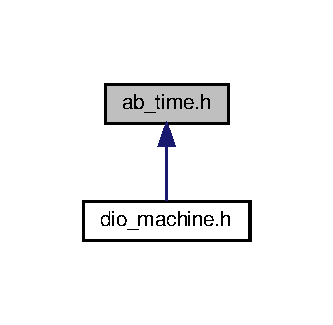
\includegraphics[width=160pt]{df/d0d/ab__time_8h__dep__incl}
\end{center}
\end{figure}
\subsection*{Typedefs}
\begin{DoxyCompactItemize}
\item 
typedef timespec \hyperlink{ab__time_8h_adc59735fd0d20e93fe3016c8b6a4f782}{abt\+\_\+time}
\end{DoxyCompactItemize}
\subsection*{Functions}
\begin{DoxyCompactItemize}
\item 
void \hyperlink{ab__time_8h_a55589396a22562f4037d2817a579e82e}{abt\+\_\+\+Get\+Current} (\hyperlink{ab__time_8h_adc59735fd0d20e93fe3016c8b6a4f782}{abt\+\_\+time} $\ast$Now)
\item 
\hyperlink{ab__time_8h_adc59735fd0d20e93fe3016c8b6a4f782}{abt\+\_\+time} \hyperlink{ab__time_8h_a410389a8363dbb7453520927331297d0}{abt\+\_\+\+Get\+Current} ()
\item 
\hyperlink{ab__time_8h_adc59735fd0d20e93fe3016c8b6a4f782}{abt\+\_\+time} \hyperlink{ab__time_8h_ad401e90e9886fe9e1fb5f49f2b11d8c0}{abt\+\_\+\+Get\+Monotonic} ()
\item 
\hyperlink{ab__common_8h_afaa62991928fb9fb18ff0db62a040aba}{u32} \hyperlink{ab__time_8h_ad3ab740dfcc9875efe4b1721fd374db4}{abt\+\_\+\+Get\+Elapsed\+Ms\+U32} (\hyperlink{ab__time_8h_adc59735fd0d20e93fe3016c8b6a4f782}{abt\+\_\+time} Start\+Time, \hyperlink{ab__time_8h_adc59735fd0d20e93fe3016c8b6a4f782}{abt\+\_\+time} Now)
\item 
\hyperlink{ab__common_8h_aafa04bc3cb166e826b75a23f4add4b59}{r32} \hyperlink{ab__time_8h_a9834c3b5b55da0fe4ae280550cf5d97f}{abt\+\_\+\+Get\+Elapsed\+Ms\+R32} (\hyperlink{ab__time_8h_adc59735fd0d20e93fe3016c8b6a4f782}{abt\+\_\+time} Start\+Time, \hyperlink{ab__time_8h_adc59735fd0d20e93fe3016c8b6a4f782}{abt\+\_\+time} Now)
\item 
\hyperlink{ab__time_8h_adc59735fd0d20e93fe3016c8b6a4f782}{abt\+\_\+time} \hyperlink{ab__time_8h_a126f380942c7e3e87802634893590928}{abt\+\_\+\+Get\+Wall\+Clock\+From\+Elapsed} (\hyperlink{ab__time_8h_adc59735fd0d20e93fe3016c8b6a4f782}{abt\+\_\+time} Start\+Time, \hyperlink{ab__common_8h_aafa04bc3cb166e826b75a23f4add4b59}{r32} Timestamp\+Ms)
\item 
\hyperlink{ab__common_8h_afaa62991928fb9fb18ff0db62a040aba}{u32} \hyperlink{ab__time_8h_ab8ae3038f353a3a59bc79abf35dcb4a4}{abt\+\_\+\+Get\+Ms\+From\+Time\+U32} (\hyperlink{ab__time_8h_adc59735fd0d20e93fe3016c8b6a4f782}{abt\+\_\+time} Time)
\item 
\hyperlink{ab__common_8h_afaa62991928fb9fb18ff0db62a040aba}{u32} \hyperlink{ab__time_8h_a05feba1d586786dad132d87c70acf336}{abt\+\_\+\+Get\+Ms\+From\+Time32} (\hyperlink{ab__time_8h_adc59735fd0d20e93fe3016c8b6a4f782}{abt\+\_\+time} Time)
\end{DoxyCompactItemize}


\subsection{Typedef Documentation}
\mbox{\Hypertarget{ab__time_8h_adc59735fd0d20e93fe3016c8b6a4f782}\label{ab__time_8h_adc59735fd0d20e93fe3016c8b6a4f782}} 
\index{ab\+\_\+time.\+h@{ab\+\_\+time.\+h}!abt\+\_\+time@{abt\+\_\+time}}
\index{abt\+\_\+time@{abt\+\_\+time}!ab\+\_\+time.\+h@{ab\+\_\+time.\+h}}
\subsubsection{\texorpdfstring{abt\+\_\+time}{abt\_time}}
{\footnotesize\ttfamily typedef timespec \hyperlink{ab__time_8h_adc59735fd0d20e93fe3016c8b6a4f782}{abt\+\_\+time}}



\subsection{Function Documentation}
\mbox{\Hypertarget{ab__time_8h_a55589396a22562f4037d2817a579e82e}\label{ab__time_8h_a55589396a22562f4037d2817a579e82e}} 
\index{ab\+\_\+time.\+h@{ab\+\_\+time.\+h}!abt\+\_\+\+Get\+Current@{abt\+\_\+\+Get\+Current}}
\index{abt\+\_\+\+Get\+Current@{abt\+\_\+\+Get\+Current}!ab\+\_\+time.\+h@{ab\+\_\+time.\+h}}
\subsubsection{\texorpdfstring{abt\+\_\+\+Get\+Current()}{abt\_GetCurrent()}\hspace{0.1cm}{\footnotesize\ttfamily [1/2]}}
{\footnotesize\ttfamily void abt\+\_\+\+Get\+Current (\begin{DoxyParamCaption}\item[{\hyperlink{ab__time_8h_adc59735fd0d20e93fe3016c8b6a4f782}{abt\+\_\+time} $\ast$}]{Now }\end{DoxyParamCaption})}

\mbox{\Hypertarget{ab__time_8h_a410389a8363dbb7453520927331297d0}\label{ab__time_8h_a410389a8363dbb7453520927331297d0}} 
\index{ab\+\_\+time.\+h@{ab\+\_\+time.\+h}!abt\+\_\+\+Get\+Current@{abt\+\_\+\+Get\+Current}}
\index{abt\+\_\+\+Get\+Current@{abt\+\_\+\+Get\+Current}!ab\+\_\+time.\+h@{ab\+\_\+time.\+h}}
\subsubsection{\texorpdfstring{abt\+\_\+\+Get\+Current()}{abt\_GetCurrent()}\hspace{0.1cm}{\footnotesize\ttfamily [2/2]}}
{\footnotesize\ttfamily \hyperlink{ab__time_8h_adc59735fd0d20e93fe3016c8b6a4f782}{abt\+\_\+time} abt\+\_\+\+Get\+Current (\begin{DoxyParamCaption}{ }\end{DoxyParamCaption})}

\mbox{\Hypertarget{ab__time_8h_a9834c3b5b55da0fe4ae280550cf5d97f}\label{ab__time_8h_a9834c3b5b55da0fe4ae280550cf5d97f}} 
\index{ab\+\_\+time.\+h@{ab\+\_\+time.\+h}!abt\+\_\+\+Get\+Elapsed\+Ms\+R32@{abt\+\_\+\+Get\+Elapsed\+Ms\+R32}}
\index{abt\+\_\+\+Get\+Elapsed\+Ms\+R32@{abt\+\_\+\+Get\+Elapsed\+Ms\+R32}!ab\+\_\+time.\+h@{ab\+\_\+time.\+h}}
\subsubsection{\texorpdfstring{abt\+\_\+\+Get\+Elapsed\+Ms\+R32()}{abt\_GetElapsedMsR32()}}
{\footnotesize\ttfamily \hyperlink{ab__common_8h_aafa04bc3cb166e826b75a23f4add4b59}{r32} abt\+\_\+\+Get\+Elapsed\+Ms\+R32 (\begin{DoxyParamCaption}\item[{\hyperlink{ab__time_8h_adc59735fd0d20e93fe3016c8b6a4f782}{abt\+\_\+time}}]{Start\+Time,  }\item[{\hyperlink{ab__time_8h_adc59735fd0d20e93fe3016c8b6a4f782}{abt\+\_\+time}}]{Now }\end{DoxyParamCaption})}

\mbox{\Hypertarget{ab__time_8h_ad3ab740dfcc9875efe4b1721fd374db4}\label{ab__time_8h_ad3ab740dfcc9875efe4b1721fd374db4}} 
\index{ab\+\_\+time.\+h@{ab\+\_\+time.\+h}!abt\+\_\+\+Get\+Elapsed\+Ms\+U32@{abt\+\_\+\+Get\+Elapsed\+Ms\+U32}}
\index{abt\+\_\+\+Get\+Elapsed\+Ms\+U32@{abt\+\_\+\+Get\+Elapsed\+Ms\+U32}!ab\+\_\+time.\+h@{ab\+\_\+time.\+h}}
\subsubsection{\texorpdfstring{abt\+\_\+\+Get\+Elapsed\+Ms\+U32()}{abt\_GetElapsedMsU32()}}
{\footnotesize\ttfamily \hyperlink{ab__common_8h_afaa62991928fb9fb18ff0db62a040aba}{u32} abt\+\_\+\+Get\+Elapsed\+Ms\+U32 (\begin{DoxyParamCaption}\item[{\hyperlink{ab__time_8h_adc59735fd0d20e93fe3016c8b6a4f782}{abt\+\_\+time}}]{Start\+Time,  }\item[{\hyperlink{ab__time_8h_adc59735fd0d20e93fe3016c8b6a4f782}{abt\+\_\+time}}]{Now }\end{DoxyParamCaption})}

\mbox{\Hypertarget{ab__time_8h_ad401e90e9886fe9e1fb5f49f2b11d8c0}\label{ab__time_8h_ad401e90e9886fe9e1fb5f49f2b11d8c0}} 
\index{ab\+\_\+time.\+h@{ab\+\_\+time.\+h}!abt\+\_\+\+Get\+Monotonic@{abt\+\_\+\+Get\+Monotonic}}
\index{abt\+\_\+\+Get\+Monotonic@{abt\+\_\+\+Get\+Monotonic}!ab\+\_\+time.\+h@{ab\+\_\+time.\+h}}
\subsubsection{\texorpdfstring{abt\+\_\+\+Get\+Monotonic()}{abt\_GetMonotonic()}}
{\footnotesize\ttfamily \hyperlink{ab__time_8h_adc59735fd0d20e93fe3016c8b6a4f782}{abt\+\_\+time} abt\+\_\+\+Get\+Monotonic (\begin{DoxyParamCaption}{ }\end{DoxyParamCaption})}

\mbox{\Hypertarget{ab__time_8h_a05feba1d586786dad132d87c70acf336}\label{ab__time_8h_a05feba1d586786dad132d87c70acf336}} 
\index{ab\+\_\+time.\+h@{ab\+\_\+time.\+h}!abt\+\_\+\+Get\+Ms\+From\+Time32@{abt\+\_\+\+Get\+Ms\+From\+Time32}}
\index{abt\+\_\+\+Get\+Ms\+From\+Time32@{abt\+\_\+\+Get\+Ms\+From\+Time32}!ab\+\_\+time.\+h@{ab\+\_\+time.\+h}}
\subsubsection{\texorpdfstring{abt\+\_\+\+Get\+Ms\+From\+Time32()}{abt\_GetMsFromTime32()}}
{\footnotesize\ttfamily \hyperlink{ab__common_8h_afaa62991928fb9fb18ff0db62a040aba}{u32} abt\+\_\+\+Get\+Ms\+From\+Time32 (\begin{DoxyParamCaption}\item[{\hyperlink{ab__time_8h_adc59735fd0d20e93fe3016c8b6a4f782}{abt\+\_\+time}}]{Time }\end{DoxyParamCaption})\hspace{0.3cm}{\ttfamily [inline]}}

\mbox{\Hypertarget{ab__time_8h_ab8ae3038f353a3a59bc79abf35dcb4a4}\label{ab__time_8h_ab8ae3038f353a3a59bc79abf35dcb4a4}} 
\index{ab\+\_\+time.\+h@{ab\+\_\+time.\+h}!abt\+\_\+\+Get\+Ms\+From\+Time\+U32@{abt\+\_\+\+Get\+Ms\+From\+Time\+U32}}
\index{abt\+\_\+\+Get\+Ms\+From\+Time\+U32@{abt\+\_\+\+Get\+Ms\+From\+Time\+U32}!ab\+\_\+time.\+h@{ab\+\_\+time.\+h}}
\subsubsection{\texorpdfstring{abt\+\_\+\+Get\+Ms\+From\+Time\+U32()}{abt\_GetMsFromTimeU32()}}
{\footnotesize\ttfamily \hyperlink{ab__common_8h_afaa62991928fb9fb18ff0db62a040aba}{u32} abt\+\_\+\+Get\+Ms\+From\+Time\+U32 (\begin{DoxyParamCaption}\item[{\hyperlink{ab__time_8h_adc59735fd0d20e93fe3016c8b6a4f782}{abt\+\_\+time}}]{Time }\end{DoxyParamCaption})\hspace{0.3cm}{\ttfamily [inline]}}

\mbox{\Hypertarget{ab__time_8h_a126f380942c7e3e87802634893590928}\label{ab__time_8h_a126f380942c7e3e87802634893590928}} 
\index{ab\+\_\+time.\+h@{ab\+\_\+time.\+h}!abt\+\_\+\+Get\+Wall\+Clock\+From\+Elapsed@{abt\+\_\+\+Get\+Wall\+Clock\+From\+Elapsed}}
\index{abt\+\_\+\+Get\+Wall\+Clock\+From\+Elapsed@{abt\+\_\+\+Get\+Wall\+Clock\+From\+Elapsed}!ab\+\_\+time.\+h@{ab\+\_\+time.\+h}}
\subsubsection{\texorpdfstring{abt\+\_\+\+Get\+Wall\+Clock\+From\+Elapsed()}{abt\_GetWallClockFromElapsed()}}
{\footnotesize\ttfamily \hyperlink{ab__time_8h_adc59735fd0d20e93fe3016c8b6a4f782}{abt\+\_\+time} abt\+\_\+\+Get\+Wall\+Clock\+From\+Elapsed (\begin{DoxyParamCaption}\item[{\hyperlink{ab__time_8h_adc59735fd0d20e93fe3016c8b6a4f782}{abt\+\_\+time}}]{Start\+Time,  }\item[{\hyperlink{ab__common_8h_aafa04bc3cb166e826b75a23f4add4b59}{r32}}]{Timestamp\+Ms }\end{DoxyParamCaption})}


\hypertarget{Readme_8md}{}\doxysection{Readme.\+md File Reference}
\label{Readme_8md}\index{Readme.md@{Readme.md}}

%--- End generated contents ---

% Index
\backmatter
\newpage
\phantomsection
\clearemptydoublepage
\addcontentsline{toc}{chapter}{Index}
\printindex

\end{document}
